\documentclass [12pt,letterpaper]{report}

% Standard packages
\usepackage{amsmath}		% Extra math definitions
\usepackage{graphics}		% PostScript figures
\usepackage{setspace}		% 1.5 spacing
\usepackage{longtable}          % Tables spanning pages
\DeclareGraphicsExtensions{.pdf,.png,.jpg,.mps}
\usepackage{amssymb}
\usepackage{mathtools}
\usepackage{ amsmath, bm }
\usepackage{graphicx}
\usepackage{epstopdf}
\usepackage{yhmath}
\usepackage{multirow}
\usepackage{dsfont}
\usepackage{bbm}
\usepackage{float}
\usepackage[section]{placeins}


% Custom packages
\usepackage[first]{datestamp}	% Datestamp on first page of each chapter
\usepackage[fancyhdr]{McECEThesis}	% Thesis style
\usepackage{McGillLogo}		% McGill University crest

% $Id: ThesisEx.tex,v 1.1 2005/06/09 12:48:46 kabal Exp $

\usepackage{color}
\def\headrulehook{\color{red}}		% Color the header rule

%===== page layout
% Define the side margins for a right-side page
\insidemargin = 1.3in
\outsidemargin = 0.8in

% Above margin is space above the header
% Below margin is space below footer
\abovemargin = 1.1in
\belowmargin = 0.75in

\newcommand{\rmnum}[1]{\romannumeral #1}
\newcommand{\Rmnum}[1]{\expandafter\@slowromancap\romannumeral #1@}
\makeatother

\newcommand\bigfrown[2][\textstyle]{\ensuremath{%
  \array[b]{c}\text{\scalebox{2}{$#1\frown$}}\\[-1.3ex]#1#2\endarray}}

%========= Document start

\begin {document}

%===== Title page

\title{The Extended Neyman-Pearson Hypotheses Testing Framework and its Application to Spectrum Sensing in Cognitive Wireless Communication}
\author{An Jiang}
\date{\Month\ \number\year}
\organization{%
  \\[0.2in]
  \McGillCrest {!}{1in}\\	% McGill University crest
  \\[0.1in]
  Department of Electrical \& Computer Engineering\\
  McGill University\\
  Montreal, Canada}
\note{%
  {\color{red} \hrule height 0.4ex}
  \vskip 3ex
  A thesis submitted to McGill University in partial fulfillment of the
  requirements for the degree of Master of Engineering (M.Eng) in Electrical Engineering.
  \vskip 3ex
  \copyright\ \the\year\ An Jiang
}

\maketitle

%===== Justification, spacing for the main text
\raggedbottom
%\onehalfspacing
\doublespacing
\pagenumbering{roman}

%===== Abstract, Sommaire & Acknowledgments
\section*{\centering Abstract}
We propose a Modified Extended Neyman Pearson (MENP) framework which is suitable for spectrum sensing when there might be different types of primary signals. Our work generalizes existing Neyman Pearson (NP) test to multiple probability of false alarm constraints. This allows the cognitive radio wireless communication system to provide different levels of protection for various primary users.  
M-ROC surface, representing the relationship between the probability of detection and the constraints, is used to depict the performance of MENP testing.   

Using MENP framework, an energy based spectrum detector and a cyclostationary based spectrum detector, are developed to detect OFDM signals. These detectors are designed to have the largest probability of detection under any probability of false alarm constraints.  

Performance analyses were performed to study the M-ROC surface behavior for both detectors. We then evaluate the improvement of the probability of detection with respect to the increase of probability of false alarms.  
The performance analysis also confirms that the optimal decision rule of energy based spectrum detector can be derived in terms of the inverse CDF of Chi-Square distribution.  

\newpage

\section*{\centering Acknowledgments}

Thesis regulations require that contributions by others in the collection of
 materials and data, the design and construction of apparatus, the performance
 of experiments, the analysis of data, and the preparation of the thesis be
 acknowledged.

%========== Tables of contents, figures, tables
\tableofcontents
\listoffigures
\listoftables

\newpage
\chapter*{List of Acronyms}\markright{List of Terms}

\begin{longtable}{ll}
  AWGN    &   Additive White Gaussian Noise\\
  CDMA    &   Code Division Multiple Access\\
  CP      &   Cyclic Prefix\\
  ENP     &   Extended Neyman Pearson\\
  MENP    &   Modified Extended Neyman Pearson\\
  MROC    &   Modified Receiver Operating Characteristic\\
  OFDM    &   Orthogonal Frequency Division Multiplexing\\
  ROC     &   Receiver Operating Characteristic
\end{longtable}

\cleardoublepage
\pagenumbering{arabic}

%========== Chapters
\typeout{}
\chapter{Introduction}
Future wireless communication systems will require higher transmission speed in order to deliver large amount of data \cite{pelcat20133gpp}. The main obstacle for providing high speed wireless communication services is the limitation of available radio frequency resources. In order to make radio systems use the radio spectrum more efficiently than in the past, advanced technologies are created, such as Cognitive Radio (CR) \cite{federal2005notice}. 

A CR is an intelligent wireless communication system which is able to monitor its operating spectrum environments and change its transmitter parameters to best match these conditions \cite{wang2011advances, a001}. It provides a novel approach for the coexistence of different wireless communication systems in the same frequency band. In a CR communication system, users are divided into two types: primary users and secondary users. A primary user is a legacy user, or a licensed user, who has priority on the particular frequency band. The CR system must ensure highly reliable communications whenever and wherever needed by primary users \cite{a001}. Potential primary users may include cellphone communication systems (e.g., GSM, CDMA or LTE), Satellite TV Broadcast systems, microphone communication systems etc.. A secondary user, or a cognitive user, is referred to someone who has lower priority to access the particular frequency band. A secondary user can utilize the spectrum only when the particular frequency is idle, and has to vacate the frequency band as soon as any primary user becomes active. 
In order to monitor the utilization of the spectrum in real-time, a spectrum sensing functionality must be introduced into a CR communication system \cite{buddhikot2007understanding, tandra2009spectrum}.   

Spectrum sensing refers to the task of identifying vacant frequency channel in a certain radio frequency band and detecting the primary users with high probability \cite{umar2012spectrum}. 
%A spectrum sensing system includes at least one measuring device and at least one testing device. The role of measuring device is transferring the RF stimuli into a suitable test statistics. The role of testing device is decide the spectrum state according to the output(s) of measuring device(s).
Spectrum sensing system can be divided into single-user sensing (local detection) and cooperative sensing \cite{wang2011advances, akyildiz2011cooperative, ma2008soft, axell2010overview}. In single-user sensing, the system makes a decision about the status of a frequency channel based on the observation from one cognitive device. The main advantage of single user sensing is its low hardware complexity. However, it has been shown that its performance deteriorates significantly in challenging propagation environments (e.g. multipath fading channel, shadowing) \cite{akyildiz2011cooperative}. In such scenarios, cooperative sensing is preferred. Cooperative sensing is a detection methods where multiple sensing device cooperate to detect the status of a radio frequency channel \cite{ganesan2005cooperative, arslan2007cognitive}. While cooperative sensing improves detection performance in challenging environments, it requires a more complicated system design,  longer sensing time,  and increased energy consumption \cite{akyildiz2011cooperative}.  
Moreover, the communication between sensing devices can lead to extra spectrum usage. 
Various sensing methods have been considered for identifying spectrum usage opportunities. Main sensing techniques include  energy detection, cyclostationary detection and waveform detection. 

Energy based detection is the simplest spectrum sensing techniques, that has been extensively used in radiometers \cite{cabric2004implementation, poor1994introduction, urkowitz1967energy}. It employs the energy of received signal to identify the channel status. Since it does not require complicated digital signal processing, it has low energy consumption and low hardware complexity.  Another favorable aspect of an energy detector is that it does not require  any information about the primary user's signal.  
The shortcomings of an energy detector include: (1) the long time to detect a  primary user if the SNR is low; (2) requires information about the variance of noise, which in some case is hard to estimate; (3) performance is not satisfying in multipath channels \cite{akyildiz2011cooperative}; (4) unable to detect spread spectrum signals like CDMA \cite{urkowitz1967energy, akyildiz2011cooperative}. 
In \cite{akyildiz2011cooperative} the authors show that the first three problems can be mitigated by diversity gain from cooperation,  making it a suitable techniques in cooperative sensing for non-CDMA signals.  

Cyclostationarity feature based detector identifies the spectrum status by exploiting autocorrelation properties of the received signals, induced by its periodicity features \cite{goldsmith2009breaking}. Such periodicity features are induced by  sinusoidal carriers,  regularly transmitted pulse trains, pilot sequences and cyclic prefixes (CP) in OFDM signals \cite{akyildiz2011cooperative, umar2013comparative}.  
Comparison with an energy detection, a cyclostationary based detector is more robust to noise uncertainty and has better performance in the low SNR regime \cite{umar2013comparative}. However since a cyclostationarity detector requires high timing accuracy when sampling, the hardware is more complex than that of an energy detector \cite{yucek2009survey}. Another disadvantage of cyclostationarity based detector is that its performance over fading channels is not satisfying \cite{tandra2007snr}.   

Waveform based detection identifies the channel status by exploiting known patterns in the primary user's signal, such as pilot sequences. The favourable aspect of such a detector is that it can achieve a high probability of detection in a comparatively short time and is able to provide  good performance in a shadowing environment \cite{tang2005some}. However, since the detector needs to extract the pilot sequence, it relies on dedicated synchronization and accurate information about the primary user's signal structure.  

%Matched filter based detector has the similar structure as a primary user receiver. Even in low SNR environment, it can still achieve a relatively high probability of detection in a short detection time \cite{tandra2005fundamental}. However since it needs to demodulate the received signal, it requires perfect information of primary signal \cite{yucek2009survey}. Another unfavorable aspect of this detector is its high power consumption, which results from its complicated hardware structure.  

%Recent years, new sensing algorithms and digital signal processing techniques have been introduced for specific spectrum sensing situations. One of them is wavelets based detection \cite{tian2007compressed, sun2013wideband, sun2013wideband2}. In wavelets based detection, sub-Neyquist sampling and compressed sensing are used to estimate the power spectrum density in a wide band channel. After that it exploits wavelets to detect the power spectrum density (PSD) edges, which correspond to transition from a occupied status to a idle status, and to estimate the power between each edges. In this way, the wideband spectrum utilization is known and the secondary users can exploit one or several idle sub-bands to communicate. 

In order to detect a free frequency channel, a spectrum sensing scheme solves a binary hypotheses testing problem, where one hypothesis refers to the event that a user is not using the channel and the other hypothesis refers to the event that a user is occupying the channel. If the a-prior probabilities of null and alternative hypotheses are known, then such a problem can be solved by using a Bayesian framework \cite{poor1994introduction}. The situation when Baysian framework could be used is considered in \cite{zeng2010review}, where  the performance of such scheme is analyzed.
Even though the Baysian framework can be used in some situations, in more often cases, the a-prior probabilities are not available. In such situations Neyman Pearson testing is employed \cite{poor1994introduction}.When there is a single type of primary user (two hypotheses), NP testing will achieve the largest probability of detecting a vacant channel when no primary user is present under a constraint on the probability that the channel will be declared vacant when in fact a primary user is present.
Traditional NP testing has been extensively used for two hypotheses problems. In such cases,  the performance is characterized by the Receiver Operating Characteristic (ROC) curve, which represents the relationship between probability of detection and probability of false alarm \cite{poor1994introduction}. 

\section{Thesis Objectives}
In spectrum sensing application, there may be more than one type of primary users. For example in IEEE 802.22  the channel can be occupied by Analog-TV Digital-TV and wireless microphone\cite{shellhammer2008spectrum}. 
In such cases, an extended NP (ENP) test  \cite{LehmannTest} can provide important advantages. A detector based on ENP testing can ensure the largest probability of detection under a separate constraint of false alarm for each primary user type \cite{LehmannTest}.
With an ENP detector, the achievable false alarm probabilities are limited. This motivates us to analyze the properties of the ENP test and propose the Modified Extended Neyman Pearson (MENP) test, that circumvents the limitations of the false alarm probabilities. Furthermore, we also consider some theoretical  findings for spectrum sensing applications.  

\section{Thesis Organization and Contribution}
The Thesis is organized as follows. We review the ENP framework and propose the MENP framework in Chapter 2. In particular,  we consider  a necessary condition proof for an  ENP test followed by  two lemmas concerning the ROC surface of ENP tests. 
We then presents Modified Extended Neyman Pearson framework aiming to  achieve the largest probability of detection  under any probability of false alarm constraints.
Then an algorithm which aims at achieving the MENP parameters is reviewed. 

In Chapter 3, M-ROC, the figure depicting the relationship between probability of detection and probability of false alarm constraints, is considered.  We then present two examples of M-ROC surfaceone associated with a Gaussian problem and the other with a Chi-Square problem. 

Once the MENP framework is presented, we apply MENP framework to energy based detection and cyclostationary based detection in Chapter 4. We consider  performances of both detectors for the situation when there are two primary users.  

Chapter 5 provides a summary of this thesis, and recommends some directions for future work.  

The contributions of this thesis are:

$\bullet$ Proved a necessary condition for the Extended Neyman Pearson Lemma (\rmnum{3}) when the probability density functions (PDFs) of given hypotheses satisfy certain constraints. 

$\bullet$ Derived the normal direction vector for a point on the ROC surface. 

$\bullet$ Proposed a novel detection scheme MENP test, which generalizes the Extended Neyman Pearson test to  achieve the largest probability of detection under any probability of false alarm constraints. 

$\bullet$ Developed numerical results to show the performance of MENP test under Gaussian situations and Chi-Square situations. 

$\bullet$ Using MENP test, energy based detector and cyclostationary based detector are derived to detect spectrum hole in the presence of multiple primary users. 


%========== Chapter 2
\typeout{}
\chapter{Extended Neyman Pearson Test}

\newcommand{\bom}{\boldsymbol{\omega}}
This chapter will start by introducing the Extended Neyman Pearson Framework. A few properties concerning ENP test will be shown. The limitation of ENP framework will come after that. Following that is a section which detailedly present Modified Extended Neyman Pearson (MENP) Framework. The new scheme aims to achieve the largest probability of detection under any possible probability of false alarm constraints. Then an algorithm which aims at achieving the MENP parameters will be reviewed. Computer simulation results, which illustrate the performance of the algorithm, will be presented. 



%========================Extended Neyman Pearson 
\typeout{}
% chapter 2 section 1
\section{The Extended Neyman Pearson Hypotheses Test}
The theories of hypotheses testing have been a subject of continuous studies over years, and have found applications in various fields such as radar systems, spectrum sensing for cognitive communication systems, and in  medical science \cite{ma2008soft, srinivasan1986distributed, spielman1973refutation}. One type of hypotheses testing problem can be abstracted as  follows: assume $M+1$  hypotheses $H_0$, $H_1$, ..., $H_{M}$, inducing $M+1$  Probability Density Functions (PDFs) on the observable $Y$,
\begin{equation}
\label{equ:hypothesis}
\begin{split}
H_0:\;\;\;\;\;\;\;\;\;&Y \sim f_0(y) \\
H_1:\;\;\;\;\;\;\;\;\;&Y \sim f_1(y)\\
&......\\
H_M:\;\;\;\;\;\;\;\;\;&Y \sim f_M(y)\\
\end{split}
\end{equation}

Based on $y$, a realization of $Y$, the detector needs to decide whether or not it comes from $f_0(y)$. A framework for solving this problem for $M=1$ was introduced in \cite{neyman1933problem} and it is commonly known as Neyman Pearson (NP) testing \cite{neyman1933problem}. The theory of NP testing was further developed for $M \geq 2$ in \cite{wald1939contributions} and \cite{dantzig1951fundamental}.  A comprehensive exposition of such generalized NP testing can be found in \cite{LehmannTest}.

\noindent  \textbf{The Extended Neyman Pearson (ENP) Lemma:}

\textit{
  Let $f_0(x), f_1(x), ..., f_{M}(x)$ be real Borel measurable functions  defined on a finite dimensional Euclidean Space $\mathcal{R}$, such that $\int \limits_\mathcal{R} | f_i(x)|\mathrm{d}x < \infty (i=0, 1,...,M)$.  Suppose that for given constants $c_1,...,c_M$ there exists a class of subsets $\mathcal{S}$, denoted $\mathcal{C}_\mathcal{S}$, such that for every $\mathcal{S} \in \mathcal{C}_\mathcal{S}$ we have
\begin{equation}
\label{one}
\int\limits_\mathcal{S} f_i(x)\mathrm{d}x = c_i, \;\;\;\;\;\;i=1,...,M
\end{equation}
Then:
%No. 1
\\\textnormal{(\rmnum{1})} Among all members of $\mathcal{C}_\mathcal{S}$ there exists one that maximizes
\[
\int \limits_\mathcal{S} f_{0}(x)\mathrm{d}x.
\]
%No.2
\\\textnormal{(\rmnum{2})} A sufficient condition for a member of $\mathcal{C}_\mathcal{S}$ to maximize
\[
\int \limits_\mathcal{S} f_{0}(x)\mathrm{d}x.
\]
is the existence of constants $k_1,...,k_M$ such that
\begin{equation}
\label{2}
f_{0}(x)>\sum\limits_{j=1}^M k_j f_j(x)\;\;\;\;\text{when $x \in \mathcal{S}$}
\end{equation}
\begin{equation}
\label{3}
f_{0}(x)<\sum\limits_{j=1}^M k_j f_j(x)\;\;\;\;\text{when $x \notin \mathcal{S}$}
\end{equation}
%No. 3
\\\textnormal{(\rmnum{3})} If a member of $\mathcal{C}_\mathcal{S}$ satisfies  \textnormal{(\ref{2})} and \textnormal{(\ref{3})} with $k_1,...,k_M\geq0$, then it maximizes
\begin{equation}
\label{4}
\int \limits_\mathcal{S} f_{0}(x)\mathrm{d}x
\end{equation}
among all $\mathcal{S}$ satisfying
\begin{equation}
\label{5}
\int \limits_\mathcal{S} f_i(x)\mathrm{d}x\leq c_i,\;\;\;\;i=1,...,M.
\end{equation}
%no. 4
\\\textnormal{(\rmnum{4})} The set $\mathcal{V}_\mathcal{M}$ of points in $M$-dimensional space whose coordinates are 
\begin{equation}
(\int_{\mathcal{S}}f_1(x)\mathrm{d}x, ..., \int_{\mathcal{S}}f_M(x)\mathrm{d}x)
\end{equation}
for any $\mathcal{S}$ is convex and closed. If $(c_1, ..., c_M)$ is an inner point of $\mathcal{V}_\mathcal{M}$, then a  necessary condition for a member of $\mathcal{C}_\mathcal{S}$ to maximize 
\[
\int \limits_\mathcal{S} f_{0}(x)\mathrm{d}x.
\]
is that there exists $M$ constants $k_1, ..., k_M$ such that \eqref{2} \eqref{3} holds a.e..
}

The associated probability of detection, $P_d$ and false alarms $P_{f_i}$ for a certain subset $\mathcal{S}$ are defined as
\cite{neyman1933problem}, 
\begin{equation}
\begin{split}
P_d &= P(H_0 | H_0) = \int_{\mathcal{S}}f_0(x)\mathrm{d}x\\
P_{f_1} &= P(H_0 | H_1) = \int_{\mathcal{S}}f_1(x)\mathrm{d}x\\
&......\\
P_{f_M} &= P(H_0 | H_M) = \int_{\mathcal{S}}f_M(x)\mathrm{d}x
\end{split}
\end{equation}

 Define the step function
\begin{equation}
   \label{equ: step function}
   u(x) = \begin{cases}
     0\;\;\;\;\;\;&x < 0\\
     0.5\;\;\;\;\;\;&x=0\\
     1\;\;\;\;\;\;&x>0\,,
   \end{cases}
\end{equation}
then for a subset $\mathcal{S}$ satisfying \eqref{2} and \eqref{3} we have:
\begin{equation}
\label{equ: pf and pd}
\begin{split}
&P_d = \int_{-\infty}^{\infty} u(f_0(x) - \sum_{j=1}^{M}k_jf_j(x)) f_0(x)\mathrm{d}x	\,, \\
&P_{f_i} = \int_{-\infty}^{\infty} u(f_0(x) - \sum_{j=1}^{M}k_jf_j(x)) f_i(x) \mathrm{d}x\;\;	 i=1, 2, ..., M\,.
\end{split}
\end{equation}
The relationship between $P_d$ and $P_{f_i}$ can be represented by Receiver Operating Characteristic (ROC) surface \cite{LehmannTest}.

From to \eqref{2} \eqref{3}, the ENP Decision rule $\delta$ is

\begin{equation}
\label{equ: decision rule}
\delta: f_0(x) \substack{H_0 \\ \geq \\ < \\ \bar{H}_0}  \sum_{j=1}^{M} k_jf_j(x)
\end{equation}

From the  \textbf{ENP Lemma}, $\delta$  achieves the largest $P_d$ under the constraints $P_{f_i} = c_i (i = 1, 2, ..., M)$.
When $M=1$, it achieves the largest $P_d$ under the constraint $P_f \leq c$ \cite{LehmannTest}, which is the well known and commonly used form of the NP test.

% notes from Prof. Leib.
For applications in spectrum sensing, $H_0$ denotes the hypothesis that the channel is free and $H_m \;(m=1, ..., M)$ corresponds to the hypothesis that the channel is occupied by the $m$-th primary signal. Although we have $M$ hypotheses, we intend to determine if the channel is free or not. Hence we need  a binary test of deciding $H_0$ versus $\bar{H}_0$ such that $P_d$ is maximized under the constraints $P_{f_m} \leq c_m$ $m = 1, ..., M$. In context of spectrum sensing, $1-P_{f_m}$ can be interpreted as the protection level of the $m-$th primary signal. The larger is this protection level, the smaller is the probability that when the $m-$th signal is active, the test will not detect it and will declare the channel free. In context of spectrum sensing, the solution of the ENP problem maximizes the probability of detecting a free channel under a constraint on the protection level for each primary signal. The protection levels of primary signals can be different and they are guaranteed.


%========================ENP Properties 
\typeout{}
% This is chapter 2 section 2

\section{Properties of ENP Test}
This section presents an example and three Lemmas to illustrate the properties of the ENP test. 

\subsection{An Example}
Assume three hypotheses given as:
\begin{equation}
  \label{2015jan29a2}
\begin{split}
H_0:\;\;\;\;&X \sim \mathcal{N}(-1, 1)\\
H_1:\;\;\;\;&X \sim \mathcal{N}(0, 1)\\
H_2:\;\;\;\;&X \sim \mathcal{N}(1, 1)
\end{split}
\end{equation}
where $\mathcal{N}(\mu, \epsilon^2)$ denotes a Gaussian PDF with mean $\mu$ and variance $\epsilon^2$. In the following, we compute the ROC surface for problem \eqref{2015jan29a2}.  
From \eqref{equ: pf and pd} we can see the expression of $P_{f_1} $, $P_{f_2}$ and $P_d$ can be written in form of  
\begin{equation}
  \begin{split}
	P_{f_1} &= \int_{-\infty}^{\infty}u(f_0(x) - k_1f_1(x) -k_2f_2(x))f_1(x)\mathrm{d}x\\
	P_{f_2} &= \int_{-\infty}^{\infty}u(f_0(x) - k_1f_1(x) -k_2f_2(x))f_2(x)\mathrm{d}x\\
	P_d     &= \int_{-\infty}^{\infty}u(f_0(x) - k_1f_1(x) -k_2f_2(x))f_0(x)\mathrm{d}x\,.
  \end{split}
  \label{2015jan29a1}
\end{equation}

By increasing $k_1$ and $k_2$ from $-30$ to $30$ with step $0.05$ separately, we can calculate the associated $P_{f_1}, P_{f_2}$ and $P_d$ from \eqref{2015jan29a1}. The ROC surface is presented in Fig. \ref{fig: 2.1}. 

\begin{figure}[!t]
\centering
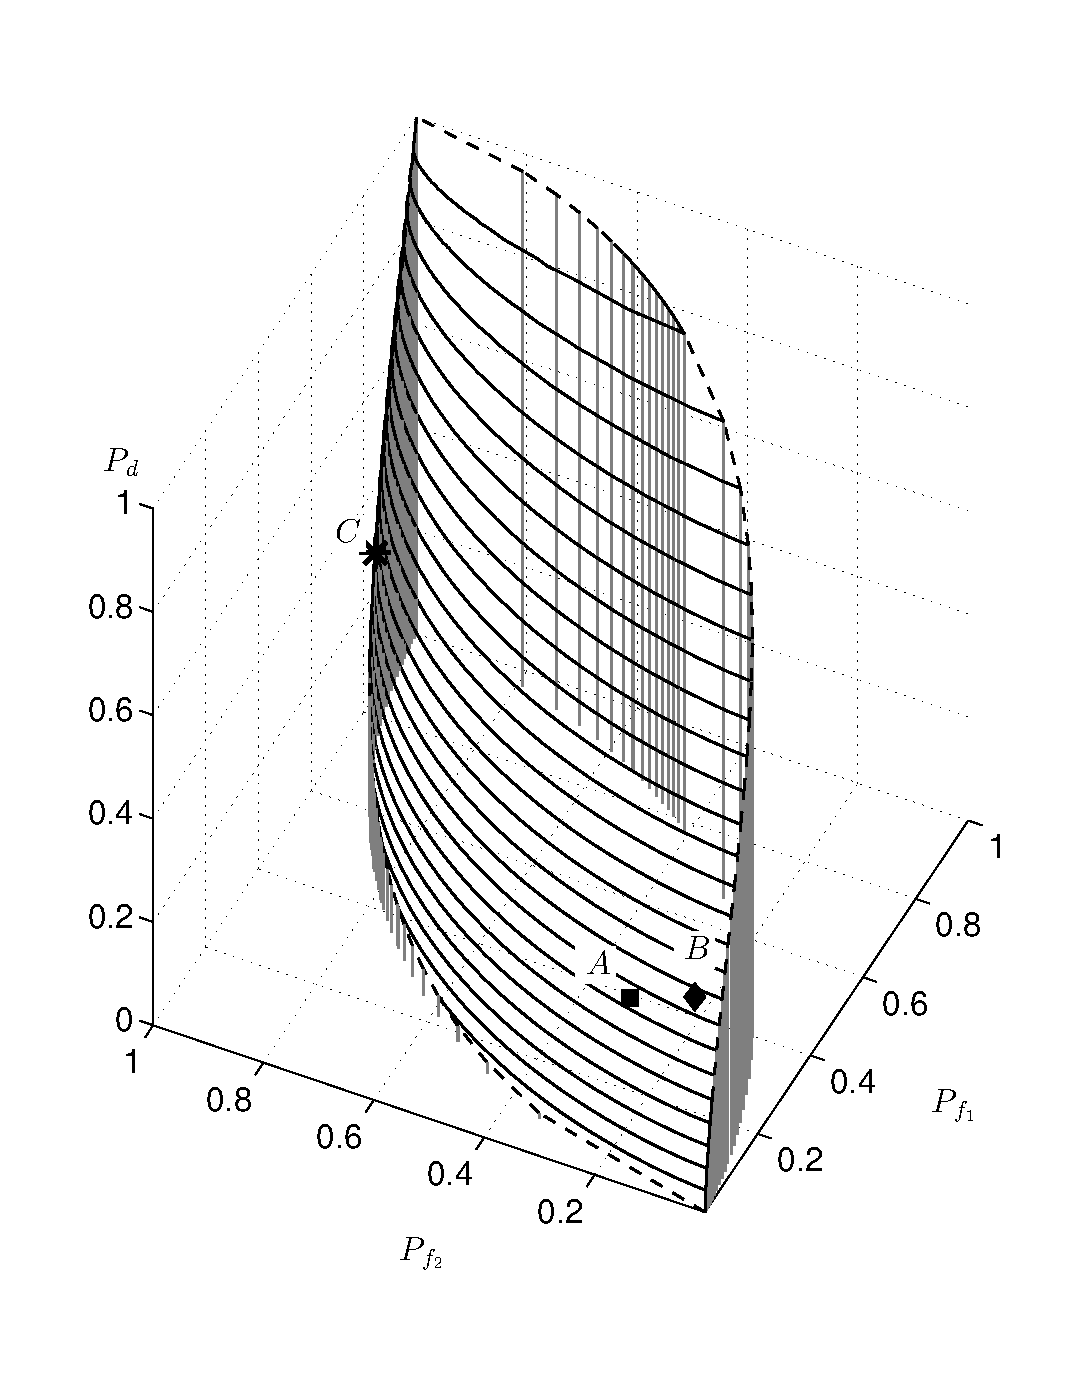
\includegraphics[width = 12cm, height=16cm]{2/c21.eps}
\caption{The ROC surface for $k_1$, $k_2$ range from $-30$ to $30$ with step $0.05$}
\label{fig: 2.1}
\end{figure}

It is interesting to observe that under ENP test framework, for a given $(P_{f_1}, P_{f_2})$  ($P_{f_1}, P_{f_2}\in [0, 1]$) the associated $P_d$ may not exists. This is because for a given $c_1, c_2 \in [0, 1]$, it is possible that there is no decision rule can satisfy
\[
  P_{f_1} = \int_{\mathcal{S}}f_1(x)\mathrm{d}x =  c_1
\]
and
\[
  P_{f_2} = \int_{\mathcal{S}}f_2(x)\mathrm{d}x = c_2
\]
at the same time. In such case, the corresponding $P_d$ does not exist. 
For example, assume $c_1 = 1$ and $c_2 = 0$. In order to satisfy 
\[
  P_{f_1} = \int_{\mathcal{S}}f_1(x)\mathrm{d}x = 1\,,
\]
set $\mathcal{S}$  must  be the whole real line, i.e. $\mathcal{S} = (-\infty, \infty)$. However in such case, we have
\[
  P_{f_2} = \int_{\mathcal{S}}f_2(x)\mathrm{d}x = 1 \neq 0
\]
Hence we can see there is no decision rule can satisfy $P_{f_1} = 1$ and $P_{f_2} = 0$ at the same time, which makes the corresponding $P_d$ do not exist.
Recall in the case of binary hypotheses testing (Traditional Neyman Pearson Test), for a given $P_f \in [0, 1]$, there always exists a corresponding $P_d$. 
% Need to change the coordinates of point A B and C.
% This is because we changed all the figures in 
Now let us consider points $A$ and $B$ on the ROC surface, which are marked with '$\blacksquare$' and '$\blacklozenge$', respectively.  The coordinate of point $A$ is $(P_{f_1}, P_{f_2}, P_d) = (0.0841, 0.1761, 0.2868)$; and the coordinate of point $B$ is  $(P_{f_1}, P_{f_2}, P_d) = (0.0807, 0.0570, 0.3344)$. We can see even through $P_{f_1}$ and $P_{f_2}$ of point $A$ is larger than that of point $B$, the probability of detection of point $A$ is  smaller than that of point $B$.  
Unlike NP test, where $P_d$ is always non-decreasing with $P_f$, in the case of multiple hypotheses testing (Extended Neyman Pearson Test), $P_d$ is not always a non-decreasing function of  $P_{f_i}$ ($i=1, ..., M$).

Finally we consider point $C$ on the ROC surface, which is marked by '$\ast$'. The coordinate of point $C$ is $(P_{f_1}, P_{f_2}, P_d) = (0.7291, 0.9454, 0.3819)$. We can observe, in this case the value of $P_d$ is smaller than the value of $P_{f_1}$ and $P_{f_2}$, i.e. under ENP test framework, $P_d \geq P_{f_i}$  ($i = 1, ..., M$) does not always hold (Qian Zhang arrives at the same conclusion in  \cite{zhang1999design, zhang2000efficient} using a different method). 

\subsection{Three Lemmas for the ENP Test}

Next we presents three lemmas concerning the properties of the ENP test.

\noindent \textbf{Lemma 1}
\noindent \textit{
Let $f_0$, $f_1$, ..., $f_M$ be PDFs defined on set $\mathcal{D}$ and $f_0(x) \neq 0$ holds a.e. on $\mathcal{D}$. For given constants $c_1, ..., c_M \in (0, 1)$, let $\mathcal{C}_\delta$ denote a set of decision rules,  such that for $\delta \in \mathcal{C}_\delta$, we have $P_{f_i} \leq c_i$.
%No. 1
%\\\textnormal{(\rmnum{1})} Among all members of $\mathcal{C}_\mathcal{S}$ there exists one that maximizes $P_d$.
%No.2
If  $\delta^{\ast}$ is a member of $\mathcal{C}_\delta$ and it maximize $P_d$ among all members of $\mathcal{C}_\delta$, then there exists non-negative constants $k_1, ..., k_M$ such that $\delta^\ast$ can be written in form of  
\begin{equation}
f_0(x) \substack{H_0 \\ \geq \\ < \\ \bar{H}_0} \sum_{j=1}^{M}k_jf_j(x)
\end{equation}
Moreover, under decision rule $\delta^\ast$ if  $P_{f_i} < c_i$, then $k_i = 0$. 
}

Qian Zhang also arrives at the conclusion that if $P_{f_i} < c_i$, then $k_i = 0$ in \cite{zhang1999design, zhang2000efficient} through analysing the performance of $P_d$ with respect to $k_i$. In the following we will prove \textbf{Lemma 1} using a mathematical method such that used in \cite{LehmannTest, dantzig1951fundamental} to prove the ENP Lemma (\rmnum{4}).

\noindent\textbf{PROOF}
\newcommand{\bmu}{\boldsymbol{\mu}}
We start by defining 
 some notations for easy presentation.
Define $\mathbf{c}^T = [c_1, c_2, ..., c_M]$, $\boldsymbol{\mu}_0^T = [\mu_1, ..., \mu_M]$, $\mathbf{k}^T = [k_1, k_2, ..., k_M]$ and  $\mathbf{P}_f^T = [P_{f_1}, P_{f_2}, ..., P_{f_M}]$ that are vectors in an $M$ dimensional Euclidean  space. Let $\bmu^T = [\bmu_0, \mu_{M+1}]$ denote a vector in $M+1$ dimensional Euclidean space. 

Let $F(\boldsymbol{\mu}_0)$ denote the largest $P_d$ under the constraints $P_{f_i} = \mu_i\;\;i = 1, ..., M$.
Let $G(\boldsymbol{\mu}_0)$ denote the largest $P_d$ under the constraints $P_{f_i} \leq \mu_i\;\;i = 1, ..., M$.
Let $P_d(\delta)$, $P_{f_i}(\delta)$ denote the $P_d$ and $P_{f_i}$ achieved by using decision rule $\delta$.
By $\mathbf{A} \leq \mathbf{B}$, $\mathbf{A} = \mathbf{B}$ and  $\mathbf{A} \geq \mathbf{B}$ we mean that every element of $\mathbf{A}$ is no larger than, equal to and no smaller than its corresponding element of $\mathbf{B}$, respectively. 
By $\mathbf{A} \neq 0$, we mean that every element of $\mathbf{A}$ is not equal to $0$. 
Let $G'$ denote the hyper surface in $M+1$ dimensional Euclidean Space defined by 
\begin{equation}
 \label{def: G'}
 G' = \{(\bmu_0, \mu_{M+1})  | \bmu_0 \in [0, 1]^M, \mu_{M+1}= G(\bmu_0) \}\,.
\end{equation}
Let $G_s$ denote the set of points in $M+1$ Euclidean space defined as 
\begin{equation}
  \label{2015feb16n1}
G_s =  \{(\boldsymbol{\mu}_0, \mu_{M+1}) | \boldsymbol{\mu}_0\in [0, 1]^M, \mu_{M+1} \in [0, G(\mathbf{\bmu_0})]
    \}\,.
  \end{equation}
  From \eqref{def: G'} and \eqref{2015feb16n1}, it can be seen $G' \in G_s$. Fig. \ref{fig: feb18} depicts the relationship between $G'$ and $G_s$ when $M=2$. In Fig. \ref{fig: feb18}, $G'$ is the surface enclosed by curve $\stackrel\frown{AC}$, curve $\stackrel\frown{AD}$, segment $\overline{OC}$ and segment $\overline{OD}$. Set $G_s$ is the space enclosed by plane $ABC$, plane $ABD$, plane $COD$ and surface $G'$.  

\begin{figure}[!t]
\centering
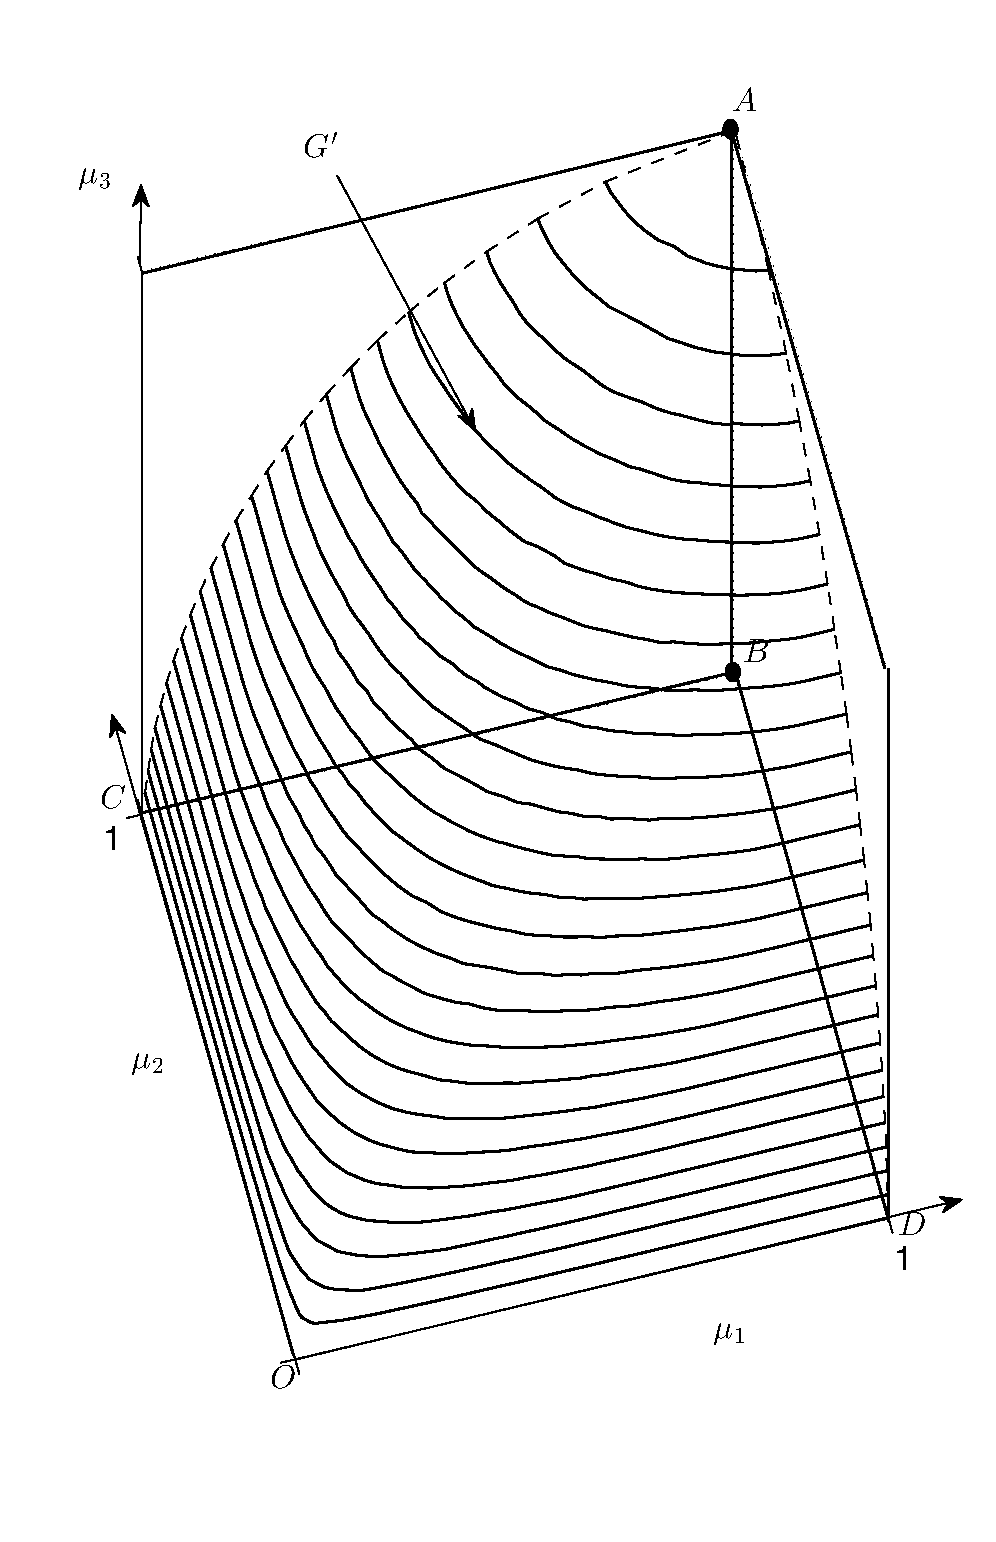
\includegraphics[width = 12cm, height=16cm]{2/example_pic.eps}
\caption{Relationship between $G'$ and $G_s$}
\label{fig: feb18}
\end{figure}
Let us define the set of points in $M+1$ dimensional Euclidean
\begin{equation}
\begin{split}
  \mathcal{N} = \{(\mu_1, \mu_2, ..., \mu_{M+1}) &| \mu_i = \int_{\mathcal{S}}f_i(x)\mathrm{d}x \;\;i=1, ..., M,\\
                                            &  \mu_{M+1}=\int_{\mathcal{S}}f_{0}(x)\mathrm{d}x \;\;\text{ for an $\mathcal{S}$}\}
\end{split}
\end{equation}
We can see that $\mathcal{N}$ is the set of point $(\bmu_0, \mu_{M+1})=(\mathbf{P}_f(\delta), P_d(\delta))$, where $\delta$ is a decision rule. Moreover, from the definition of $\mathcal{N}$ and $F(\bmu_0)$ we can conclude that for a point $(\bmu_0, \mu_{M+1}) \in \mathcal{N}$, we have $\mu_{M+1} \leq F(\bmu_0)$. 
To see it, assume $\mu_{M+1} > F(\bmu_0)$. Then there is a decision rule $\delta$ such that $P_{f_i}(\delta) = \mu_i$ ($i=1, ..., M$) and $P_d(\delta) > F(\bmu_0)$. This is contradictory with the definition of $F(\bmu_0)$. 

The whole proof consists of the following parts: first we prove $G(\boldsymbol{\mu}_0)$ is a convex, non-decreasing function, and when $\boldsymbol{\mu}_0 > 0$, $G(\boldsymbol{\mu}_0) > 0$;
secondly it will be shown that $G_s$ is a convex set and $\mathcal{N} \subseteq G_s$; 
after that we will illustrate for a point $(\mu_1^0, \mu_2^0, ..., \mu_{M+1}^0) \in G'$, there exists a non-negative $\mathbf{k}$ such that 
\[
\mu_{M+1} - \sum_{i=1}^{M}k_i\mu_i \leq \mu_{M+1}^0 - \sum_{i=1}^{M}k_i\mu_i^0
\]
holds for point $(\mu_1, \mu_2, ..., \mu_{M+1}) \in G_s$;
in the end, we will show for $\mathbf{c} \in (0, 1)$, there exists non-negative $\mathbf{k}$ such that the optimal decision rule to achieve the largest $P_d$ under constraint $\mathbf{P}_f \leq \mathbf{c}$ can be written in form of 
\[
f_0(x) \substack{H_0 \\ > \\ < \\ \bar{H}_0} \sum_{i=1}^{M}k_if_i(x)\,.
\]

Firstly we will prove $G(\bmu_0)$ is a convex non-decreasing function for $\bmu_0 \in [0, 1]^M$.
 Let $\boldsymbol{\mu}^1$ and  $\boldsymbol{\mu}^2$ be two points on $G'$ with coordinates $(\boldsymbol{\mu}^1_0, \mu_{M+1}^1)$ and $(\boldsymbol{\mu}^2_0, \mu_{M+1}^2)$, i.e. $\mu_{M+1}^1 = G(\boldsymbol{\mu}_0^1)$ and $\mu_{M+1}^2 = G(\boldsymbol{\mu}_0^2)$. Let $\delta_1$ be a decision rule which can achieve the largest $P_d$ under the constraint $\mathbf{P}_f \leq \boldsymbol{\mu}_0^1$ and $\delta_2$ be a decision rule which can achieve the largest $P_d$ under the constraint $\mathbf{P}_{f} \leq \boldsymbol{\mu}_0^2$. Thus we can see 
 \begin{subequations}
\begin{align}
&\mu_{M+1}^1 = P_d(\delta^1) = G(\boldsymbol{\mu}_0^1)\\
&\mu_{M+1}^2 = P_d(\delta^2)=G(\boldsymbol{\mu}_0^1)\\
&\mathbf{P}_f(\delta^1) \leq \boldsymbol{\mu}^1_0\\
&\mathbf{P}_f(\delta^2) \leq \boldsymbol{\mu}^2_0
\end{align}
 \end{subequations}
 
Construct a new randomized test $\delta^3$, where $\delta^1$ and $\delta^2$ are used with equal probability. With decision rule $\delta^3$, we have 
\begin{subequations}
\begin{align}
\label{1120night1}
&P_d(\delta^3) = 0.5P_d(\delta^1)+0.5P_d(\delta^2) = 0.5G(\bmu_0^1) + 0.5G(\bmu_0^2)\\
&\mathbf{P}_{f}(\delta^3) = 0.5\mathbf{P}_f(\delta^1)+0.5\mathbf{P}_f(\delta^2) \leq 0.5\boldsymbol{\mu}^1_0 + 0.5\boldsymbol{\mu}^2_0
\end{align}
\end{subequations}
Let $\delta'$ denote the optimal decision rule for 
 \begin{equation}
 \begin{split}
 \label{1120t}
 \max&\;\;\;\;P_d\\
 \text{s.t.}&\;\;\;\;\mathbf{P}_f \leq 0.5\boldsymbol{\mu}^1_0 + 0.5\boldsymbol{\mu}^2_0
 \end{split}
 \end{equation}
then obviously $P_d(\delta') \geq P_d(\delta^3)$ (otherwise $\delta'$ cannot be the optimal decision rule for \eqref{1120t}).The optimal $P_d$ of \eqref{1120t} can be written as $G(0.5\boldsymbol{\mu}^1_0 + 0.5\boldsymbol{\mu}^2_0)$, hence we have  
\begin{equation}
\label{1120t2}
G(0.5\boldsymbol{\mu}^1_0 + 0.5\boldsymbol{\mu}^2_0) \geq  P_d(\delta^3).
\end{equation}
Substitute \eqref{1120night1} into above equation, we can see
\begin{equation}
\label{1120t3}
G(0.5\boldsymbol{\mu}^1_0 + 0.5\boldsymbol{\mu}^2_0) \geq 0.5 G(\boldsymbol{\mu}^1_0)+ 0.5 G(\boldsymbol{\mu}^2_0)\,.
\end{equation}
Equation \eqref{1120t3} implies $G(\bmu_0)$ is a convex function for $\bmu_0 \in [0, 1]^M$.

According to the definition of $G(\bmu_0)$, when $\mu_i$ increases, the false alarm constraints are relaxed, 
so the value of $G(\bmu_0)$ will either remain the same or increase. 
This suggests $G(\bmu_0)$ is a non-decreasing function of $\bmu_0$. 
This is not contradictory with the conclusion that 
$P_d$ is not always increasing with $P_{f_i}\;\;(i=1, 2, \cdots, M)$  (we arrived at this conclusion in Chapter 2 section 1.1 on page 12).  This is because $\bmu_0$ is not the probability of false alarms but rather the constraints of the probability of false alarm. 

Next we will show when $\boldsymbol{\mu}_0 > 0^M$, the value of $G(\boldsymbol{\mu}_0)$ is strictly larger than zero.
Let $\delta^\ast$ be the optimal decision rule for $\bmu_0$. By optimal  we mean that this decision rule provides the largest $P_d$ under the constraints $\mathbf{P}_f \leq \bmu_0$, i.e. $P_d(\delta^\ast) = G(\bmu_0)$. Consider two decision rule $\delta^1$ and $\delta^2$ defined as 
\begin{equation}
  \label{2015feb09a4}
  \delta^1:\;\; \begin{cases}
    &x \;\;\;\text{belongs to $H_0$ if } x \in \emptyset \\
    &x \;\;\;\text{belongs to $\bar{H}_0$ if } x \in \mathcal{D}
  \end{cases}
\end{equation}
and
\begin{equation}
  \label{2015feb09a5}
  \delta^2:\;\; \begin{cases}
    &x \;\;\;\text{belongs to $H_0$ if } x \in \mathcal{D} \\
    &x \;\;\;\text{belongs to $\bar{H}_0$ if } x \in \emptyset
  \end{cases}
\end{equation}

From \eqref{2015feb09a4} and \eqref{2015feb09a5} we can see the $P_d$ and $P_{f_i}$ under under decision rule $\delta^1$ and $\delta^2$ can be written as
\begin{equation}
  P_d(\delta^1) = \int_{\emptyset}f_0(x)\mathrm{d}x = 0
\end{equation}
\begin{equation}
    P_{f_i}(\delta^1) = \int_{\emptyset}f_i(x)\mathrm{d}x = 0
\end{equation}
\begin{equation}
    P_d(\delta^2) = \int_{\mathcal{D}}f_0(x)\mathrm{d}x = 1
\end{equation}
\begin{equation}
    P_{f_i}(\delta^2) = \int_{\mathcal{D}}f_i(x)\mathrm{d}x = 1
\end{equation}

Let $\mu_{min} = \min(\mu_1, \mu_2, \cdots, \mu_M)$, since $\bmu_0 > 0^M$, it can be seen $\mu_{min} > 0$. Construct a new randomized test $\delta^3$ where $\delta^1$ and $\delta^2$ are used with probability $1 - \mu_{min} $ and $\mu_{min}$. With decision rule $\delta^3$ we have
\begin{equation}
  P_d(\delta^3) = (1 - \mu_{min})P_d(\delta^1) + \mu_{min}P_d(\delta^2) = \mu_{min} > 0
\end{equation}
\begin{equation}
  P_{f_i}(\delta^3) = (1 - \mu_{min})P_{f_i}(\delta^1) + \mu_{min}P_{f_i}(\delta^2) = \mu_{min} \leq \mu_i \;\;\;\;(i = 1, 2, \cdots, M)
\end{equation}

Hence we can see by using $\delta^3$ we have
\[
  \mathbf{P}_f(\delta^3) \leq \bmu_0\,.
\]
Since $\delta^\ast $ is the optimal decision rule for $\bmu_0$, we can conclude $P_d(\delta^\ast) \geq  P_d(\delta^3) = \mu_{min} >  0$. Since $G(\bmu_0) = P_d(\delta^\ast)$, we can conclude $G(\bmu_0) > 0$ when $\bmu_0 > 0 $. 


In the following, we consider the property of $G_s$. First we will prove that $G_s$ is a convex set. 
Let $\boldsymbol{\mu}^1$ and  $\boldsymbol{\mu}^2$ be two points belongs to $G_s$ with coordinates $(\boldsymbol{\mu}^1_0, \mu_{M+1}^1)$ and $(\boldsymbol{\mu}^2_0, \mu_{M+1}^2)$. According to the definition of $G_s$, we have 
\begin{subequations}
\label{1120t4}
\begin{align}
\label{1120night6}
&0^M \leq \bmu_0^1 \leq 1^M\\
\label{1120night7}
&0^M \leq \boldsymbol{\mu}^2_0 \leq 1^M\\
\label{1120night3}
&0 \leq \mu_{M+1}^1 \leq G(\boldsymbol{\mu}_0^1)\\
\label{1120night4}
&0 \leq \mu_{M+1}^2 \leq G(\boldsymbol{\mu}_0^2)
\end{align}
\end{subequations}

Let $\boldsymbol{\mu}^3$ be the middle point between $\boldsymbol{\mu}^1$ and $\boldsymbol{\mu}^2$ with coordinate $(\bmu_0^3, \mu_{M+1}^3)$, where  
\begin{subequations}
\label{1120t5}
\begin{align}
\label{1120night5}
\bmu_0^3 &= 0.5\boldsymbol{\mu}_0^1 + 0.5 \boldsymbol{\mu}_0^2\\
\label{1120night2}
\mu_{M+1}^3 &= 0.5 \mu_{M+1}^1 + 0.5 \mu_{M+1}^2
\end{align}
\end{subequations}
In the following, we will show $\bmu^3 \in G_s$.  
From \eqref{1120night6}, \eqref{1120night7} and \eqref{1120night5} we can see that
\begin{equation}
\label{equ: 1120n1}
\bmu_0^3 \in [0, 1]^M
\end{equation}
Substituting \eqref{1120night3} \eqref{1120night4} into \eqref{1120night2}, we have
\begin{equation}
  \label{equ:2015feb1a}
0 \leq \mu_{M+1}^3 \leq 0.5 G( \bmu_0^1) + 0.5G(\bmu_0^2)\,.
\end{equation} 
Using \eqref{1120t3} and \eqref{1120night5} with \eqref{equ:2015feb1a} gives,
\begin{equation}
\label{equ: 1120n}
0 \leq \mu_{M+1}^3 \leq G(0.5 \bmu_0^1 + 0.5\bmu_0^2) = G(\bmu_0^3)\,.
\end{equation}
From \eqref{equ: 1120n} and \eqref{equ: 1120n1}, it can be conclude 
 $\bmu^3 \in G_s$, hence $G_s$  is a convex set.  

Next we prove $\mathcal{N} \subseteq G_s$. We need to show that if  $\forall (\mu_1, ..., \mu_{M+1}) \in \mathcal{N}$, then this point also belongs to $G_s$.
Assume $(\mu_1^0, ..., \mu_{M+1}^0)$ is a point in $\mathcal{N}$. 
In previous discussion, it has been shown $\mu_i^0 \in [0, 1]$ ($i = 1, ..., M$) and $\mu_{M+1}^0 \in [0, F(\bmu_0^0)]$, where $\bmu_0^0 = [\mu_1^0, ..., \mu_M^0]$. 
According to the definition of $G(\bmu_0)$ and $F(\bmu_0)$, we can conclude $G(\bmu_0^0) \geq F(\bmu_0^0)$. 
This implies $\mu_{M+1}^0 \in [0, G(\bmu_0^0)]$ and we have  
\begin{equation}
\begin{split}
&\mu_i^0 \in [0, 1]\;\;\;\;(i=1, 2, ..., M)\\
&\mu_{M+1}^0 \in [0, G(\bmu_0^0)]
\end{split}
\end{equation}
The above equation suggests point $(\mu_1^0, ..., \mu_{M+1}^0)$ also belongs to set $G_s$.
Hence we proved $\mathcal{N} \subseteq G_s$. 

In the following we will show for point $(\mu_1^0, \mu_2^0, ..., \mu_{M+1}^0)$ that belongs to $G'$ ($\mu_i^0 \in (0, 1), i = 1, 2, ..., M$), there exists a non-negative $\mathbf{k}$ such that  
\[
\mu_{M+1} - \sum_{i=1}^{M}k_i\mu_i \leq \mu_{M+1}^0 - \sum_{i=1}^{M}k_i\mu_i^0
\]
holds for any $(\mu_1, \mu_2, ..., \mu_{M+1}) \in G_s$, 

Assume $(\mu_0^0, \mu_1^0, ..., \mu_{M+1}^0)$ is a point on the $G'$ surface, i.e. $\mu_{M+1}^0 = G(\bmu_0^0)$, where $\bmu_0^0 = [\mu_1^0, ..., \mu_{M}^0]$. 
Also we assume $\mu_1^0, \mu_2^0, ..., \mu_M^0 \in (0, 1)$. 
According to the definition of $G_s$, for any positive $\epsilon$, point $(\mu_0^0, \mu_1^0, ..., \mu_{M+1}^0+\epsilon) \notin G_s$. Thus point $(\mu_1^0, ..., \mu_{M+1}^0)$ is a boundary point of set $G_s$.  
Since $G_s$ is a convex set and $(\mu_0^0, \mu_1^0, ..., \mu_{M+1}^0)$ is a boundary point of $G_s$,  
there exists an $M+1$-dimensional hyperplane $\Pi$ through this point such that $\Pi$ contains only boundary points of $G_s$ and $G_s$ lies entirely on one sides of $\Pi$  \cite{dantzig1951fundamental}. 
There exists $k_i^0$ ($i=1, ..., M+1$) such that the equation defining $\Pi$ can be written as \cite{dantzig1951fundamental}
\begin{equation}
\label{PI}
k_{M+1}^0\mu_{M+1} - \sum_{i=1}^{M}k_i^0\mu_i = k_{M+1}^0\mu_{M+1}^0 - \sum_{i=1}^{M}k_i^0\mu_i^0
\end{equation}

As  we have proved when $\mu^0_i\neq 0$ ($i=1, ..., M$), $\mu_{M+1}^0 = G(\bmu_0^0) $ is strictly larger than zero. Hence there exists a $\mu_{M+1}' = \frac{\mu_{M+1}^0}{2}$ such that $\mu_{M+1}' \in (0, \mu_{M+1}^0)$. From the definition of $G_s$, it is easy to see that point $(\mu^0_1, ..., \mu^0_M, \mu_{M+1}')$ also belongs to set $G_s$. Besides that, since $\mu^0_i \in (0, 1)$ ($i=1, ..., M$) and $\mu_{M+1}' \in (0, \mu_{M+1}^0)$, it can be concluded that point $(\mu_1^0, \mu_2^0, ..., \mu_{M+1}')$ is an inner point of $G_s$.
From previous discussion, we can see point $(\mu^0_1, ..., \mu^0_M, \mu_{M+1}')$ is not contained in hyperplane $\Pi$, i.e.
\[
k_{M+1}^0\mu_{M+1}' - \sum_{i=1}^{M}k_i^0\mu_i^0 \neq k_{M+1}^0\mu_{M+1}^0 - \sum_{i=1}^{M}k_i^0\mu_i^0
\]
\[
\therefore k_{M+1}^0\mu_{M+1}' \neq k_{M+1}^0\mu_{M+1}^0
\]
\[
\therefore k_{M+1}^0 \neq 0
\]
With $k_i = \frac{k_i^0}{k_{M+1}^0}$, the equation defining the hyperplane $\Pi$ can be written as
\begin{equation}
\label{PI2}
\mu_{M+1} - \sum_{i=1}^{M}k_i\mu_i = \mu_{M+1}^0 - \sum_{i=1}^{M}k_i\mu_i^0\,,
\end{equation}
on equivalently 
\begin{equation}
\label{PI2b}
\mu_{M+1} - \sum_{i=1}^{M}k_i\mu_i - (\mu_{M+1}^0 - \sum_{i=1}^{M}k_i\mu_i^0) = 0\,.
\end{equation}

\cite{planeside} shows $\Pi$ divides the space into two parts, on one side of $\Pi$, points satisfy
\[
\mu_{M+1} - \sum_{i=1}^{M}k_i\mu_i - (\mu_{M+1}^0 - \sum_{i=1}^{M}k_i\mu_i^0) > 0\,;
\]
on the other side of $\Pi$, points satisfy
\[
\mu_{M+1} - \sum_{i=1}^{M}k_i\mu_i - (\mu_{M+1}^0 - \sum_{i=1}^{M}k_i\mu_i^0) < 0\,.
\]

When $(\mu_1, ... ,\mu_M, \mu_{M+1})=(\mu_1^0, ..., \mu_M^0, 0)$, the left-hand of \eqref{PI2} is smaller than the right-hand, i.e.
\begin{equation}
  \begin{split}
 \mu_{M+1} - \sum_{i=1}^{M}k_i\mu_i < \mu_{M+1}^0 - \sum_{i=1}^{M}k_i\mu_i^0\\
 \mu_{M+1} - \sum_{i=1}^{M}k_i\mu_i - (\mu_{M+1}^0 - \sum_{i=1}^{M}k_i\mu_i^0) < 0\,.
 \end{split}
  \label{2015feb02a1}
\end{equation}
 Since $\mu_i^0 \in (0, 1)$, from the definition of $G_s$, we can see that point $(\mu_1, ... ,\mu_M, \mu_{M+1})=(\mu_1^0, ..., \mu_M^0, 0)$ belongs to $G_s$. 
Since point $(\mu_1, ... ,\mu_M, \mu_{M+1})=(\mu_1^0, ..., \mu_M^0, 0)$ satisfies \eqref{2015feb02a1} and since $G_s$ lies entirely on one side of hyper plane $\Pi$, to make all points belonging to $G_s$ lies on the same side of $\Pi$ as point $(\mu_1, ... ,\mu_M, \mu_{M+1})=(\mu_1^0, ..., \mu_M^0, 0)$ does, we must have
%Since $G_s$ lies entirely on one side of \eqref{PI2}, and since when $(\mu_1, ... ,\mu_M, \mu_{M+1})=(\mu_1^0, ..., \mu_M^0, 0)$, the left-hand of \eqref{PI2} is smaller than the right-hand, we must have 
\begin{equation}
\mu_{M+1} - \sum_{i=1}^{M}k_i\mu_i -  ( \mu_{M+1}^0 - \sum_{i=1}^{M}k_i\mu_i^0) \leq 0
\label{PI3}
\end{equation}
on equivalently,
\[
\mu_{M+1} - \sum_{i=1}^{M}k_i\mu_i \leq   \mu_{M+1}^0 - \sum_{i=1}^{M}k_i\mu_i^0
\]
for all the points belong to $G_s$ \cite{dantzig1951fundamental, planeside}. 

Up to now, we have proved that if  $(\bmu_0^0, \mu_{M+1}^0) \in G'$ and $\bmu_0^0 \in (0, 1)^M$, there exists constants $k_1$, ..., $k_M$ such that
\begin{equation}
\mu_{M+1} - \sum_{i=1}^{M}k_i\mu_i \leq \mu_{M+1}^0 - \sum_{i=1}^{M}k_i\mu_i^0
\label{PPI3}
\end{equation}
holds for  $(\mu_1, \mu_2, ...\mu_{M+1}) \in G_s$. In the following, we will show that the constants $k_i$ in \eqref{PPI3} must be non-negative.   

Now consider another point on $G'$ with coordinate $(\mu_1^0, ..., \mu_l^0+\epsilon, ..., \mu_M^0, \mu_{M+1}')$, where $\epsilon > 0$ and $l$ is an integer between $1$ and $M$.  Since both points $(\mu_1^0, ..., \mu_l^0, ..., \mu_M^0, \mu_{M+1}^0)$ and $(\mu_1^0, ..., \mu_l^0+\epsilon, ..., \mu_M^0, \mu_{M+1}')$ lies on $G'$, we can conclude $G([\mu_1^0, ..., \mu_l^0, ...., \mu_M^0]) = \mu_{M+1}^0$ and $G([\mu_1^0, ..., \mu_l^0 + \epsilon, ...., \mu_M^0]) = \mu_{M+1}'$. As we proved $G(\bmu_0)$ is a non-decreasing function, we must have  $\mu_{M+1}' \geq \mu_{M+1}^0$.

Substituting $(\mu_1^0, ..., \mu_l^0+\epsilon, ..., \mu_M^0, \mu_{M+1}')$ into the left side of \eqref{PPI3}, we have
\begin{equation}
\mu_{M+1}' - k_1\mu_1^0 - ... - k_l(\mu_l^0+\epsilon)- ... - k_M\mu_M^0 \leq \mu_{M+1}^0 - k_1\mu_1^0 - ... - k_l\mu_l^0- ... - k_M\mu_M^0
\end{equation}
\begin{equation}
\therefore \mu_{M+1}' - k_l(\mu_l^0+\epsilon)\leq \mu_{M+1}^0 - k_l\mu_l^0
\end{equation}
\begin{equation}
\mu_{M+1}' - \mu_{M+1}^0 \leq k_l\epsilon
\end{equation}
\begin{equation}
\therefore k_l \geq \frac{\mu_{M+1}' - \mu_{M+1}^0}{\epsilon} \geq 0 \;\;\;\;l = 1, 2, \cdots, M
\label{2015feb16a1}
\end{equation}
From \eqref{2015feb16a1} we can see that the constants $k_l$ ($l = 1, 2, \cdots, M$) in \eqref{PPI3} are non-negative.
As we have proved if  $(\bmu_0^0, \mu_{M+1}^0) \in G'$ and $\bmu_0^0 \in (0, 1)^M$, there exists constants $k_1, ..., k_M$ such that  
\begin{equation}
\mu_{M+1} - \sum_{i=1}^{M}k_i\mu_i \leq \mu_{M+1}^0 - \sum_{i=1}^{M}k_i\mu_i^0
\label{PPI32015bc}
\end{equation}
holds for  $(\mu_1, \mu_2, ...\mu_{M+1}) \in G_s$ and the constants $k_1, k_2, \cdots, k_M$ are non-negative,  
we can conclude 
if  $(\bmu_0^0, \mu_{M+1}^0) \in G'$ and $\bmu_0^0 \in (0, 1)^M$, there exists constants $k_1, ..., k_M \geq 0 $ such that  
\begin{equation}
\mu_{M+1} - \sum_{i=1}^{M}k_i\mu_i \leq \mu_{M+1}^0 - \sum_{i=1}^{M}k_i\mu_i^0
\label{PPI32015b}
\end{equation}
holds for  $(\mu_1, \mu_2, ...\mu_{M+1}) \in G_s$. 

For the given constants $\mathbf{c}$ ($\mathbf{c} \in (0, 1)^M$), 
 assume a decision rule $\delta^\ast$  achieves the largest $P_d$  while keeping $\mathbf{P}_f \leq \mathbf{c}$. In the following we will prove there exists non-negative $\mathbf{k}$  such that $\delta^\ast$ can be written in form of 
\[
f_0(x) \substack{H_0 \\ > \\ < \\ \bar{H}_0 } \sum_{i=1}^{M}k_if_i(x)\,.
\]

Let $\bmu_0 = \mathbf{c}$, according to the definition of $G'$, we can see $(\mathbf{c},G(\mathbf{c})) \in G'$.  As $\delta^\ast $ achieves the largest $P_d$ under constraint $\mathbf{P}_f \leq \mathbf{c}$, from the definition of $G(\bmu_0)$ we can see $P_{d}(\delta^\ast) = G(\mathbf{c})$. 

Since we have proved if $(\bmu_0^0, \mu_{M+1}^0) \in G'$ and $\bmu_0^0 \in (0, 1)^M$, there exists non-negative constants $k_1$, ..., $k_M$ such that
\begin{equation}
\mu_{M+1} - \sum_{i=1}^{M}k_i\mu_i \leq \mu_{M+1}^0 - \sum_{i=1}^{M}k_i\mu_i^0
\label{PPI32015}
\end{equation}
holds for all points belonging $G_s$ and $(\mathbf{c},G(\mathbf{c})) \in G'$, we can see there exists non-negative $\mathbf{k}$ such that  

%According to the definition of $G(\bmu_0)$, we can see $P_d(\delta^\ast) = G(\mathbf{c})$. Since $(\mathbf{c}, G(\mathbf{c}))$is a point on the hyper surface $G'$,  there exists non-negative $\mathbf{k}$ such that 
\begin{equation}
\label{TEMP}
\mu_{M+1} - \sum_{i=1}^{M}k_i\mu_i \leq G(\mathbf{c}) - \sum_{i=1}^{M}k_ic_i
\end{equation}
holds for $(\mu_1, \mu_2, ..., \mu_{M+1}) \in G_s$.
Since $P_{f_i}(\delta^\ast) \leq c_i$ (for $i=1, ..., M$) and $k_i \geq 0$, we know
\[
k_ic_i \geq k_iP_{f_i}(\delta^\ast)
\]
\[
\therefore \sum_{i=1}^{M}k_ic_i \geq \sum_{i=1}^{M}k_iP_{f_i}(\delta^\ast)
\]
Hence we have
\begin{equation}
\label{con: 1}
G(\mathbf{c}) - \sum_{i=1}^{M}k_ic_i \leq G(\mathbf{c}) - \sum_{i=1}^{M}k_iP_{f_i}(\delta^\ast)\,.
\end{equation}
From \eqref{TEMP} and \eqref{con: 1}, we have 
\begin{equation}
\label{equ: TEMP3}
\mu_{M+1} - \sum_{i=1}^{M}k_i\mu_i \leq G(\mathbf{c}) - \sum_{i=1}^{M}k_ic_i \leq G(\mathbf{c}) - \sum_{i=1}^{M}k_iP_{f_i}(\delta^\ast)
\end{equation}
\begin{equation}
\label{ASD}
\therefore \mu_{M+1} - \sum_{i=1}^{M}k_i\mu_i \leq G(\mathbf{c}) - \sum_{i=1}^{M}k_iP_{f_i}(\delta^\ast)
\end{equation}
Substitute $G(\mathbf{c}) = P_d(\delta^\ast)$ into \eqref{ASD}, 
\begin{equation}
\label{TEMP2}
\mu_{M+1} - \sum_{i=1}^{M}k_i\mu_i \leq P_d(\delta^\ast) - \sum_{i=1}^{M}k_iP_{f_i}(\delta^\ast)\,,
\end{equation}
where $(\mu_0, ..., \mu_{M+1}) \in G_s$.

Since $\mathcal{N} \subseteq G_s$, \eqref{TEMP2} also holds for a point belonging to $\mathcal{N}$.
According to the definition of $\mathcal{N}$, for $(\mu_1, \mu_2, ..., \mu_{M+1} \in \mathcal{N})$, we have  
\begin{equation}
\label{def: mu}
\begin{cases}
\mu_i = \int_{\mathcal{S}}f_i(x)\mathrm{d}x \;\;\;\;i = 1, ..., M\\
\mu_{M+1} = \int_{\mathcal{S}}f_{0}(x)\mathrm{d}x
\end{cases}
\end{equation}
where $\mathcal{S}$ can be any subset of domain $\mathcal{D}$. 

$P_{f_i}(\delta^\ast)$ and $P_{d}(\delta^\ast)$ can be written as
\begin{equation}
\label{def: pfd}
\begin{cases}
P_{f_i}(\delta^\ast) = \int_{\mathcal{S}^\ast}f_i(x)\mathrm{d}x\;\;\;\;i=1, ..., M\\
P_d(\delta^\ast) = \int_{\mathcal{S}^\ast}f_0(x)\mathrm{d}x
\end{cases}
\end{equation}
Substituting \eqref{def: mu} and \eqref{def: pfd} into \eqref{TEMP2}, we have: 
\[
\int_{\mathcal{S}}f_{0}(x)\mathrm{d}x - \sum_{i=1}^{M}k_i\int_{\mathcal{S}}f_i(x)\mathrm{d}x \leq \int_{\mathcal{S}^\ast}f_{0}(x)\mathrm{d}x - \sum_{i=1}^{M}k_i\int_{\mathcal{S}^\ast}f_i(x)\mathrm{d}x
\]
\[
\therefore 
\int_{\mathcal{S}}f_{0}(x)\mathrm{d}x - \sum_{i=1}^{M}\int_{\mathcal{S}}k_if_i(x)\mathrm{d}x \leq \int_{\mathcal{S}^\ast}f_{0}(x)\mathrm{d}x - \sum_{i=1}^{M}\int_{\mathcal{S}^\ast}k_if_i(x)\mathrm{d}x
\]
\begin{equation}
\label{TEMP4}
\therefore \int_{\mathcal{S}}(f_{0}(x)- \sum_{i=1}^{M}k_if_{i}(x))\mathrm{d}x \leq \int_{\mathcal{S}^\ast}(f_{0}(x)- \sum_{i=1}^{M}k_if_{i}(x))\mathrm{d}x 
\end{equation}
The integrand of the left-hand \eqref{TEMP4} and right-hand \eqref{TEMP4} are the same. In order to make \eqref{TEMP4} holds for all set $\mathcal{S}$,  
 $\mathcal{S}^\ast$ must  maximize 
\begin{equation}
\int_{\mathcal{S}}(f_{0}(x)\mathrm{d}x - \sum_{i=1}^{M}k_if_i(x))\mathrm{d}x
  \label{2015feb2a3}
\end{equation}
among all $\mathcal{S}$. To maximize \eqref{2015feb2a3}, $\mathcal{S}^\ast$ should include all the integral set when $f_{0}(x)- \sum_{i=1}^{M}k_if_{i}(x) > 0$ and exclude the integral set when $f_{0}(x)- \sum_{i=1}^{M}k_if_{i}(x) < 0$, i.e.   
 $\mathcal{S}^\ast$ satisfies
\[
x \in \mathcal{S}^\ast\;\;\;\;\text{if}\;\;\;\;f_{0}(x)- \sum_{i=1}^{M}k_if_{i}(x) > 0
\]
\[
x \notin \mathcal{S}^\ast\;\;\;\;\text{if}\;\;\;\;f_{0}(x)- \sum_{i=1}^{M}k_if_{i}(x) < 0
\]

Hence we can conclude that for a given vector of constraints for $\mathbf{P}_f$, denoted as $\mathbf{c} \in (0, 1)^M$, there exists a set of non-negative $\mathbf{k}$ such that 
the optimal decision rule can be written as 
\[
f_0(x) \substack{H_0 \\ > \\ < \\ \bar{H}_0 } \sum_{i=1}^{M}k_if_i(x)\,.
\]

Moreover, since \eqref{TEMP} holds for any point $(\mu_1, \mu_2, ..., \mu_{M+1}) \in \mathcal{N}$ and $(\mathbf{P}_f(\delta^\ast), P_d(\delta^\ast)) \in \mathcal{N}$, we can conclude 
\begin{equation}
P_d(\delta^\ast) - \sum_{i=1}^{M}k_iP_{f_i}(\delta^\ast) \leq G(\mathbf{c}) - \sum_{i=1}^{M}k_ic_i
\end{equation}
As we have shown $G(\mathbf{c}) = P_d(\delta^\ast)$, the above equation can be written as
\begin{equation}
 G(\mathbf{c}) - \sum_{i=1}^{M}k_ic_i \geq G(\mathbf{c}) - \sum_{i=1}^{M}k_iP_{f_i}(\delta^\ast)
\label{TEMP5}
\end{equation}
From \eqref{con: 1} and \eqref{TEMP5}  we can conclude
\[
G(\mathbf{c}) - \sum_{i=1}^{M}k_iP_{f_i}(\delta^\ast) =  G(\mathbf{c}) - \sum_{i=1}^{M}k_ic_i
\]
\[
\therefore  \sum_{i=1}^{M}k_iP_{f_i}(\delta^\ast) =  \sum_{i=1}^{M}k_ic_i
\]
Since $k_iP_{f_i}(\delta^\ast) \leq k_ic_i$ (for $i=1, ..., M$), the above equation can be fulfilled only if $k_iP_{f_i}(\delta^\ast) = k_ic_i$ (for $i=1, ..., M$). When for a certain $i$ $P_{f_i}(\delta^\ast) < c_i$, then $k_i$ must be zero.

Q.E.D.

Upon examination  the optimal decision rule for a given probability of false alarm constraints, in the following we consider properties of the ROC surface, embodied by two lemmas with proof.  

\noindent \textbf{Condition 1}
\textit{
\noindent Let $f_i(x) \;\;i=0, 1, ..., M$ be the PDF induced by hypothesis $H_i$, and define $g(x) = f_0(x) - \sum_{j=1}^{M} k_jf_j(x)$ where $k_i$  ($i = 1, 2, ..., M$) are real numbers. Let $\mathcal{D} \in \mathbb{R}$ be an open set such that $\int_{\bar{\mathcal{D}}}f_i(x)=0\;\;i = 1, 2, ..., M$. Furthermore,  if $x_0$ is a solution  for $g(x) = 0 \;\;(x \in \mathcal{D})$, then there exists an integer $n$ such that  the $n$-th order derivative of $g(x_0)$ is not equal to zero $(g^{(n)}(x_0) \neq 0)$.
}

\noindent \textbf{Lemma 2}
\textit{
\noindent Under}
\textbf{Condition 1}
\textit{, let $\mathbf{P}$ be a point with coordinate $(P_d, P_{f_1}, ..., P_{f_M})$ on the ROC surface of the EPN test. If there exists a tangent hyperplane at $\mathbf{P}$, then its normal is parallel to the vector $\mathbf{n} = (-1, k_1, ..., k_M)$, where $k_i$ are the parameters of the ENP test achieving $\mathbf{P}$.
}

\noindent\textbf{PROOF}
Define $\mathbf{k} = [k_1, k_2, ..., k_M]^T$ and $\mathbf{P}_f = [P_{f_1}, P_{f_2}, ..., P_{f_M}]^T$. Since both $P_d$ and $\mathbf{P}_f$ are functions of $\mathbf{k}$, $\mathbf{P}_f(\mathbf{k}_0)$ denotes the value of $\mathbf{P}_f$ when $\mathbf{k} = \mathbf{k}_0$ and $P_d(\mathbf{k}_0)$ denotes the value of $P_d$ when $\mathbf{k} = \mathbf{k}_0$. Using Taylor's expansion \cite{zill2011advanced} for $\mathbf{P}_f$ and $P_d$,
\begin{equation}
\label{pro: pd}
P_d = P_d(\mathbf{k}_0) + \frac{\mathrm{d}P_d}{\mathrm{d}\mathbf{k}^T}\bigg{|}_{\mathbf{k}=\mathbf{k_0}}(\mathbf{k} - \mathbf{k}_0)
+ o(\mathbf{k} - \mathbf{k}_0)
\end{equation}

\begin{equation}
\label{pro: pf}
\mathbf{P}_f = \mathbf{P}_f(\mathbf{k}_0) + \frac{\mathrm{d}\mathbf{P}_f}{\mathrm{d}\mathbf{k}^T}\bigg{|}_{\mathbf{k}=\mathbf{k_0}}(\mathbf{k} - \mathbf{k}_0)
+ o(\mathbf{k} - \mathbf{k}_0)
\end{equation}
here $\mathbf{k} \rightarrow \mathbf{k}_0$.

Consider the hyperplane $y$ as a function of $\mathbf{x}$ defined by
\begin{equation}
\label{pro: y}
y = P_d(\mathbf{k}_0) + \frac{\mathrm{d}P_d}{\mathrm{d}\mathbf{k}^T}\bigg{|}_{\mathbf{k}=\mathbf{k_0}}(\mathbf{z} - \mathbf{k}_0)
\end{equation}
\begin{equation}
\label{pro: x}
\mathbf{x} = \mathbf{P}_f(\mathbf{k}_0) + \frac{\mathrm{d}\mathbf{P}_f}{\mathrm{d}\mathbf{k}^T}\bigg{|}_{\mathbf{k}=\mathbf{k_0}}(\mathbf{z} - \mathbf{k}_0)
\end{equation}
The above equations construct a tangent hyperplane for the ROC surface at point $(P_d(\mathbf{k}_0), \mathbf{P}_f^T(\mathbf{k}_0))$. Combining both equations  we get

\begin{equation}
\label{pro : y2}
y = P_d(\mathbf{k}_0) + \frac{\mathrm{d}P_d}{\mathrm{d}\mathbf{k}^T}\bigg{|}_{\mathbf{k}=\mathbf{k_0}}(
\frac{\mathrm{d}\mathbf{P}_f}{\mathrm{d}\mathbf{k}^T}\bigg{|}_{\mathbf{k}=\mathbf{k_0}}
)^{-1} (\mathbf{x} - \mathbf{P}_f(\mathbf{k}_0))
\end{equation}
Hence the normal for point $(P_d(\mathbf{k}_0), \mathbf{P}_f^T(\mathbf{k}_0))$ on ROC surface can be written as
\begin{equation}
\label{vec: normal}
[-1, \frac{\mathrm{d}P_d}{\mathrm{d}\mathbf{k}^T}\bigg{|}_{\mathbf{k}=\mathbf{k_0}}(
\frac{\mathrm{d}\mathbf{P}_f}{\mathrm{d}\mathbf{k}^T}\bigg{|}_{\mathbf{k}=\mathbf{k_0}}
)^{-1}
].
\end{equation}

In the following, we will prove $ \frac{\mathrm{d}P_d}{\mathrm{d}\mathbf{k}^T}(
\frac{\mathrm{d}\mathbf{P}_f}{\mathrm{d}\mathbf{k}^T}
)^{-1} = \mathbf{k}^T
$, which can be written as
\begin{equation}
\label{pro: vec}
\frac{\mathrm{d}P_d}{\mathrm{d}\mathbf{k}^T} = \mathbf{k}^T \frac{\mathrm{d}\mathbf{P}_f}{\mathrm{d}\mathbf{k}^T}
\end{equation}
which in component form can be written as 
\begin{equation}
\label{pro: component}
\frac{\partial P_d}{\partial k_i} - \sum_{n=1}^{M}k_n\frac{\partial P_{f_n}}{\partial k_i} = 0 \;\;\;\;(i=1, 2, ..., M).
\end{equation}
Using \eqref{equ: pf and pd} and calculating the  partial derivatives results in
\begin{equation}
\label{pro: Pf par k}
\frac{\partial P_{f_n}}{ \partial k_i} = - \int_{\mathcal{D}}\delta (f_0(x) - \sum_{j=1}^{M}k_jf_j(x))f_i(x)f_n(x) \mathrm{d}x\,,
\end{equation}
\label{pro: Pd par k}
\begin{equation}\frac{\partial P_d}{ \partial k_i} = - \int_{\mathcal{D}}\delta (f_0(x) - \sum_{j=1}^{M}k_jf_j(x))f_i(x)f_0(x) \mathrm{d}x\,,
\end{equation}
where $\delta(\bullet)$ is Dirac's delta function defined as following,

\begin{equation}
\label{pro: delta}
\delta(x) = \substack{\lim \\ \epsilon \rightarrow 0} \begin{cases}
\frac{1}{\epsilon}\;\;\;\;&\text{when} \;\;x \in (-\frac{\epsilon}{2}, \frac{\epsilon}{2})\\
0\;\;\;\;&\text{otherwise}
\end{cases} \;\;\;\;
\end{equation}

Defining $g(x) = f_0(x) - \sum_{j=1}^{M} k_jf_j(x)$, \eqref{pro: component} can be written as $\int_{\mathcal{D}}\delta(g(x))g(x)f_n(x)\mathrm{d}x = 0, n = 1, ..., M$.

When $g(x) \neq 0$, we have $\delta(g(x)) = 0$ and $\delta(g(x))g(x)f_i(x) = 0$.   When  $g(x) = 0$, we can solve the equation according to the definition of $\delta(\bullet)$ and consider
\begin{equation}
\label{pro: important}
\int_{\{x|g(x)\in (-\frac{\epsilon}{2}, \frac{\epsilon}{2})\}} \frac{1}{\epsilon} g(x)f_n(x) \mathrm{d}x\;\;\;\;n= 1, ..., M
\end{equation}

Since when $g(x) \in (-\frac{\epsilon}{2}, \frac{\epsilon}{2})$, $|g(x)| < \frac{\epsilon}{2}$,
\begin{equation}|
\int_{\{x|g(x)\in (-\frac{\epsilon}{2}, \frac{\epsilon}{2})\}} \frac{1}{\epsilon} g(x)f_i(x) \mathrm{d}x | <
\int_{\{x|g(x)\in (-\frac{\epsilon}{2}, \frac{\epsilon}{2})\}} \frac{1}{2}f_i(x) \mathrm{d}x
\end{equation}

When $\epsilon$ is small enough, we have 
\[
  g(x) \in (-\frac{\epsilon}{2}, \frac{\epsilon}{2}) \Leftrightarrow  x \in (x_0 - \frac{\triangle x}{2}, x_0 + \frac{\triangle x}{2})
\]
when $x_0 $ is such that $g(x_0) = 0$, and $\triangle x \rightarrow 0$ when $\epsilon \rightarrow 0$. 

Hence when $\epsilon \rightarrow 0$ we have 

%define
\def \LEFT{ x_s
  -\left(\frac{n!\varepsilon}{2|g^{(n)}(x_s)|}\right)^{\frac{1}{n}}}
  \def \RIGHT{ x_s
  +\left(\frac{n!\varepsilon}{2|g^{(n)}(x_s)|}\right)^{\frac{1}{n}}}
%end define
\begin{equation}
\int_{\{x|g(x)\in (-\frac{\epsilon}{2}, \frac{\epsilon}{2})\}} \frac{1}{2}f_i(x) \mathrm{d}x \rightarrow
f_i(x_0)\bigtriangleup x \rightarrow 0
\end{equation}

Using the above two conclusions for $g(x) = 0$ and $g(x) \neq 0$, we get
\begin{equation}
\int_{\mathcal{D}} \delta (g(x)) g(x)f_i(x) \mathrm{d}x = 0
\end{equation}
proving that \eqref{pro: component} holds.

Q.E.D.

\noindent \textbf{Lemma 3}
\textit{
\noindent
Under}
\textbf{Condition 1}
\textit{, let $\mathbf{P}$ be a point on the ROC surface. Then $\frac{\partial P_d}{\partial P_{f_i}} \bigg|_P = k_i$, where $k_i$ are the parameters of ENP test achieving $\mathbf{P}$.
}

\noindent\textbf{PROOF}
The expression of tangent hyper surface for point $(P_d^0, P_{f_1}^0, ..., P_{f_M}^0)$ on the ROC hyper surface can be written as
\begin{equation}
P_d = P_d^0 + \sum_{i=1}^{M} \frac{\partial P_d}{\partial P_{f_i}}\bigg|_{P_{f_i} = P_{f_i}^0}(P_{f_i} - P_{f_i}^0)\,.
\end{equation}
Hence the normal at this point is

 $\mathbf{n} = [-1, \frac{\partial P_d}{\partial P_{f_1}}, \frac{\partial P_d}{\partial P_{f_2}}, ..., \frac{\partial P_d}{\partial P_{f_M}}]$. Since we have proved that  the normal for this point is $\mathbf{n} = [-1, k_1, k_2, ..., k_M]$, we must have
\begin{equation}
\frac{\partial P_d}{\partial P_{f_i}}\bigg|_{P} = k_i
\end{equation}

Q.E.D.


%========================Relationship between Neyman Pearson and Bayesian 
\typeout{}
\section{Relationship to Bayesian Hypotheses Test}
Upon examination the properties of ENP Test, this section will present the relationship between ENP Test and Bayesian Test. 

Consider the following $M+1$ hypotheses concerning an observation of $X$
\begin{equation}
\label{equ: 2 pdf}
\begin{split}
H_0:\;\;\;\;&X \sim f_0(x)\\
H_1:\;\;\;\;&X \sim f_1(x)\\
&......\\
H_{M}:\;\;\;\;&X \sim f_M(x)\,,
\end{split}
\end{equation}
where $f_i(x)$ ($i=0, 1, ..., M$) are Probability Density Functions (PDFs). 
Let $\pi_0, \pi_1, ..., \pi_M$ be the probability of occurrences of hypotheses $H_0$, $H_1$, ..., $H_M$, respectively. 
Based on $x$, a realization of $X$, a Bayesian Test $\delta_B$ is used to discriminate which hypothesis it comes from.  
Let $C_{ij}$ denote the cost incurred by choosing hypothesis $H_i$ when hypothesis $H_j$ is true. 
Let $\mathcal{C}_i$ ($i=1, ..., M$) denote a subset of $\mathbb{R}$ such that under decision rule $\delta_B$ we choose $H_i$ when $x \in \mathcal{C}_i$. 
Let $P_i(\mathcal{C}_j)$ denote the integration of $f_i(x)$ over subset $\mathcal{C}_j$, i.e. 
\[
P_i(\mathcal{C}_j) = \int_{\mathcal{C}_j} f_i(x)\mathrm{d}x\,.
\]
Before we process, we make following assumption:
\\(1) $C_{ij} = 0$ when $i \neq 0$ and $j \neq 0$
\\(2) $C_{10} = C_{20} = ... = C_{M0}$

In the following, we consider the form of $\delta_B$ under such assumption.
Let $a_0 = C_{10} = C_{20} = ... = C_{M0}$ and $a_i = C_{0i}$ ($i= 1, 2, ..., M$).
The conditional risk for Bayesian Test can be written as 
\begin{subequations}
\label{r0}
\begin{align}
\begin{split}
R_0(\delta_B) &= C_{00}P_0(\mathcal{C}_0) + C_{10}P_0(\mathcal{C}_1) + ... +  C_{M0}P_0(\mathcal{C}_M)\\
&= a_0P_0(\mathcal{C}_1) + a_0P_0(\mathcal{C}_2) + ... + a_0P_0(\mathcal{C}_M)\\
&= a_0P_0(\mathcal{C}_1\cup \mathcal{C}_2 \cup ... \cup \mathcal{C}_M)\\
&= a_0P_0(\bar{\mathcal{C}_0})\\
&= a_0(1 - P_0(\mathcal{C}_0))\\
&= a_0(1 - \int_{\mathcal{C}_0}f_0(x)\mathrm{d}x)\\
\end{split}
\begin{split}
R_1(\delta_B) &= C_{01}P_1(\mathcal{C}_0) + C_{11}P_1(\mathcal{C}_1) + ... +  C_{M1}P_1(\mathcal{C}_M)\\  
&= a_1P_1(\mathcal{C}_0)\\
&= a_1\int_{\mathcal{C}_0}f_1(x)\mathrm{d}x\\
\end{split}
......\\
\begin{split}
R_M(\delta_B) &= C_{0M}P_M(\mathcal{C}_0) + C_{1M}P_M(\mathcal{C}_1) + ... +  C_{2M}P_M(\mathcal{C}_2)\\
&= a_MP_M(\mathcal{C}_0)\\
&= a_M\int_{\mathcal{C}_0}f_{M}(x)\mathrm{d}x\,.
\end{split}
\end{align}
\end{subequations}

The total cost function $r(\delta_B)$ can be written as 
\begin{equation}
\begin{split}
\label{r00}
r(\delta_B) &= \pi_0 R_0(\delta) + \pi_1R_1(\delta) + ... +  \pi_MR_M(\delta)\\
&= \pi_0a_0 - (\pi_0a_0P_0(\mathcal{C}_0) - \pi_1a_1P_1(\mathcal{C}_0 - ... - \pi_Ma_MP_M(\mathcal{C}_0)))\\
&= \pi_0a_0 - \int_{\mathcal{C}_0}\pi_0a_0f_0(x) - \pi_1a_1f_1(x) - ... - \pi_Ma_Mf_M(x) \mathrm{d}x\,. 
\end{split}
\end{equation}
and thus we see that $r(\delta)$ is a minimum over all $\mathcal{C}_0$ if and only if 
\begin{equation}
\begin{split}
\label{equ: C}
\mathcal{C}_0 &= \{ x\in \mathcal{C}_0 | \pi_0a_0f_0(x) - \pi_1a_1f_1(x) - ... - \pi_Ma_Mf_M(x) \geq 0\}\\
&= \{ x\in \mathcal{C}_0 | f_0(x) \geq \sum_{i=1}^{M}\frac{\pi_ia_i}{\pi_0a_0}f_i(x) \}\,.
\end{split}
\end{equation}

Since $\mathcal{C}_1$, $\mathcal{C}_2$..., $\mathcal{C}_M$ can not be determined through $r(\delta_B)$,  $\delta_B$ cannot discriminate among $H_i$ ($ i = 1, ..., M$). In other words, $\delta_B$ can only distinguish between $H_0$ and $\bar{H}_0$.  Decision rule $\delta_B$ can be written in form of: 

\begin{equation}
\label{dec: minimax form}
f_0(x) \substack{H_0 \\ \geq \\ < \\ \bar{H}_0} \sum_{i=1}^{M}\frac{\pi_ia_i}{\pi_0a_0}f_i(x)\,.
\end{equation}

Assume $\pi_0 = \pi_1 = ... = \pi_{M} = \frac{1}{M+1}$, $a_0 = 1$ and $a_i = k_i$ ($i=0, 1, ..., M$), \eqref{dec: minimax form} can be written as
\begin{equation}
\label{dec: bay ney}
f_0(x) \substack{H_0 \\ \geq \\ < \\ \bar{H}_0} \sum_{i=1}^{M}k_if_i(x)\,. 
\end{equation}

It can be observed \eqref{dec: bay ney} is an ENP decision rule. This implies an ENP test
\[
f_0(x) \substack{H_0 \\ \geq \\ < \\ \bar{H}_0} \sum_{i=1}^{M}k_if_i(x)
\]
is a Bayesian test with:
\\(1) $C_{ij} = 0$ when $i \neq 0$ and $j \neq 0$;
\\(2) $C_{10} = C_{20} = ... = C_{M0} =1$;
\\(3) $C_{0i} = k_i$ ($i = 1, 2, ..., M$);
\\(4) $\pi_i = \frac{1}{M+1}$ ($i=0, 1, ..., M$).

Furthermore, by substituting $\pi_0 = \pi_1 = ... = \pi_M = \frac{1}{M+1}$, $a_0 = 1$  and $a_i = k_i$ ($i = 1, 2, ..., M$) into \eqref{r00}, the total cost function can be written as
\begin{equation}
\label{r00 2}
\begin{split}
r(\delta)&= 1 - \int_{\mathcal{C}_0}f_0(x) - \sum_{i=1}^{M}k_if_i(x)\mathrm{d}x\\
&= 1 - (\int_{\mathcal{C}_0}f_0(x)\mathrm{d}x - \sum_{i=1}^{M}k_i\int_{\mathcal{C}_0}f_i(x)\mathrm{d}x)
\end{split}
\end{equation}
Under the framework of ENP test, $P_d$ and $\mathbf{P}_f$ can be written in form of: 
\begin{equation}
\begin{split}
\label{equ: 2 pd}
P_d = \int_{\mathcal{C}_0}f_0\mathrm{d}x\\
P_{f_i} = \int_{\mathcal{C}_0}f_i\mathrm{d}x \,,
\end{split}
\end{equation}
Substitute \eqref{equ: 2 pd} into \eqref{r00 2},
\begin{equation}
\label{r00 3}
r(\delta) = 1 - (P_d - \sum_{i=1}^{M}k_iP_{f_i})\,.
\end{equation}
Previous discussion suggests an ENP test 
\[
f_0(x) \substack{H_0 \\ \geq \\ < \\ \bar{H}_0} \sum_{i=1}^{M}k_if_i(x)\,. 
\]
maximizes 
\[
r(\delta) = P_d - \sum_{i=1}^{M}k_iP_{f_i}\,.
\]
among all possible decision rules.



%========================MENP 
\typeout{}
% MENP test 

\section{Modified Extended Neyman Pearson Testing}

%define \JUDGEMENT
\def \JUDGEMENT{u(f_0(x) - \sum_{j=1}^{M}k_j f_j(x))}

In the context of spectrum sensing, following problem needs to be solve
      \begin{equation}
      \label{equ: problemstate}
      \begin{split}
      \max\;\;\;\;\;\;&P_d\\
      \text{s.t.}\;\;\;\;\;\;&\mathbf{P}_f \leq \mathbf{c}\,,
      \end{split}
      \end{equation}
where $\mathbf{c} \in (0, 1)$.

According to ENP Lemma, this problem can be solved by an ENP test only when there are parameters $k_i \geq 0, \;\;i=1, ..., M$ such that 
\begin{equation}
\label{equ: condition for ENP}
\begin{split}
c_i = \int_{-\infty}^{\infty}u(f_0 - \sum_{j=1}^{M}k_jf_j(x))f_i(x)\mathrm{d}x \;\;i = 1, ..., M
\end{split}
\end{equation}

The case when the given $c_i\;\; (i= 1, 2, ..., M)$ do not satisfy \eqref{equ: condition for ENP} was not considered so far. 

Next we present the Modified Extended Neyman Pearson Test (MENP) for solving \eqref{equ: problemstate}.

Before we proceed, we will define some notations for easy presentation.
Define the set 
\[\mathcal{A}_\mathbf{c} = \{
  \mathbf{P}_f | 0 \leq P_{f_i} \leq c_i
  \;\;i=1, 2, ..., M\}\,.
\]
and set 
\[
\alpha^+ \triangleq \{\mathbf{P}_f | P_{f_i} = \int_{-\infty}^{\infty} \JUDGEMENT f_i(x) \mathrm{d}x, \text{where\;\;} k_i \geq 0 \;\;i=1, ..., M\}\,.
\]
\noindent \textbf{Modified Extended Neyman Pearson Test}
\noindent \textit{
\\\textnormal{(\rmnum{1})} Assume $\mathbf{c} \in \alpha^+$. Then there must be a $\mathbf{k}^0 = [k_1^0, k_2^0, ..., k_M^0]^T$ with $k_i \geq 0\;\;i=1, ..., M$ satisfying
}
\begin{equation}
\label{equ:Pf}
  P_{f_i}^0 = \int_{-\infty}^{\infty} u(f_0(x) - \sum_{j=1}^{M}k_j^0f_j(x))f_i(x)\mathrm{d}x = c_i \;\; (i= 1, 2, ..., M)\,.
\end{equation}
\textit{
    and the decision rule $\delta $ solving  \eqref{equ: problemstate} is:
}
\begin{equation}
\label{equ:decision rule}
\delta:\;\;\;\;f_0(x) \substack{H_0 \\ \geq \\ < \\ \bar{H}_0} \sum_{i=1}^{M}k_i^0f_i(x)
\end{equation}
\textit{
\noindent \textnormal{(\rmnum{2})} Assuming $\mathbf{c} \notin \alpha^+$, Let $\mathcal{C} = \mathcal{A}_{\mathbf{c}} \cap \alpha^+$, and $\mathbf{a}^0 = [a_1^0, a_2^0, ..., a_M^0]^T \in \mathcal{C}$ be such that
}
\begin{equation}
\label{equ: F0}
\max_{\mathbf{a} \in \mathcal{C}}\;\;\;\;F(\mathbf{a}) = F(\mathbf{a}^0)\\
\end{equation}
\textit{
Since $\mathbf{a}^0 \in \mathcal{A}_{\mathbf{c}} \cap \alpha^+$, from \textnormal{(\rmnum{1})} we have that there exists a vector $\mathbf{k}^0$ such that \eqref{equ:decision rule}  maximizes $P_d$ under the constraints $P_{f_i} = a_i^0, \;i=1, ..., M$. Here since $a_i^0 \leq c_i^0, \;i=1, ..., M$ this decision rule  solves \eqref{equ: problemstate}.
}

Next we will show \textbf{Modified Extended Neyman Pearson Test} can provide an optimal solution for \eqref{equ: problemstate} when $f_0(x) \neq 0$ a.e. on its domain.

\textbf{PROOF}
MENP (\rmnum{1}) is a direct conclusion from ENP Lemma, we will consider MENP (\rmnum{2}). Assume $\mathbf{a}^0$ satisfy
\begin{equation}
\label{a0}
\max_{\mathbf{a}\in\mathcal{C}} F(\mathbf{a}) = F(\mathbf{a^0})
\end{equation}
and decision rule $\delta^0$ maximizes $P_d$ under the constraints $P_{f_i} = a^0_i$ ($i = 1, ..., M$). Since $\mathbf{a}^0 \in \alpha^+$, from (\rmnum{1}) we know there exists $k_1^0, ..., k_M^0$ such that $\delta^0$ can be written in form of 
\[
\delta^0:\;\;\;\;f_0(x) \substack{H_0 \\ \geq \\ < \\ \bar{H_0}} \sum_{i=1}^{M}k_i^0f_i(x)\,.
\] 
From the definition of $F(\mathbf{a})$, we know $F(\mathbf{a^0}) = P_d(\delta^0)$.

In the following, we  will prove $\delta^0$ is the optimal solution for \eqref{equ: problemstate}. 
Assume  $\delta^0$ does not achieve the largest $P_d$ under constraints $P_{f_i} \leq c_i$ ($i=1, ..., M$) and let $\delta'$ be the optimal decision rule for \eqref{equ: problemstate}, hence  we can conclude
\begin{equation}
\label{condition 1}
P_{f_i}(\delta') \leq c_i\;\;\;\;i=1, 2, ..., M\\
\end{equation}
and
\begin{equation}
\label{condition 2}
P_{d}(\delta') > P_d(\delta^0)\,.
\end{equation}
From \textbf{Lemma 1}, there exists non-negative constants $k_1', ..., k_M'$ such that $\delta'$ can be written in form of 
\begin{equation}
f_0(x) \substack{H_0 \\ \geq \\ < \\ \bar{H_0}} \sum_{i=1}^{M}k_i'f_i(x)\,.
\end{equation}
and thus $P_d(\delta')$ and $P_{f_i}(\delta')$ can be written as
\begin{equation}
\begin{cases}
\label{TEMP10}
P_{d}(\delta') &= \int_{-\infty}^{\infty} u(f_0(x) - \sum_{i=1}^{M}k_i'f_i(x)) f_0(x) \mathrm{d}x\\
P_{f_i}(\delta') &= \int_{-\infty}^{\infty} u(f_0(x) - \sum_{i=1}^{M}k_i'f_i(x)) f_i(x) \mathrm{d}x
\end{cases}
\end{equation}
where $k_i' \geq 0$.

From \eqref{condition 1} and \eqref{TEMP10}, we can conclude $\mathbf{P}_f(\delta') \in \mathcal{A}_\mathbf{c} \cap \alpha^+$. Let $\mathbf{a}' = \mathbf{P}_f(\delta')$, and we have $F(\mathbf{a}') = P_d(\delta')$. This is because $\delta'$ is an ENP test with $\mathbf{P}_f$ is equal to $\mathbf{a}'$.  

Since $P_d(\delta') > P_d(\delta^0)$, we have $F(\mathbf{a'}) > F(\mathbf{a^0})$. This is contradictory with the condition that $\mathbf{a^0}$ satisfy \eqref{a0}.

Hence we conclude $\delta^0$ is the optimal solution for \eqref{equ: problemstate}. $\blacksquare$

Next we present a look-up table method of finding $\mathbf{k}$ when $\mathbf{c} \notin \alpha^+$. For a specific $\mathbf{c}$, in order to get $\mathbf{a}^0$, we need to determine the set of $\alpha^+$. We can conduct an exhaustive search over a grid of $k_1, ..., k_M$ ($k_i \geq 0$) depending on preferable accuracy and store these results ($P_d, \mathbf{P}_f, \mathbf{k}$) into a lookup table $T_1$. After that, we iterate every item in $T_1$ and put the item into table $T_2$ if the item satisfies:  $\mathbf{P}_f \leq \mathbf{c}$.
At last, we iterate every item in $T_2$ and get the largest $P_d$ and its decision rule $\mathbf{k}$.
Obviously, the look-up table method also applies to the situation when $\mathbf{c} \in \alpha^+$. Thus we can see by searching $T_1$ we can get the decision rule for any $\mathbf{c}$.  

From above discussion, we can see if an ENP decision rule with positive parameters acquires the largest $P_d$ while keeping $\mathbf{P}_f \leq \mathbf{c}$ among all ENP test with positive parameters, it is the theoretical solution for \eqref{equ: problemstate}. 


 %========================Algorithm
\typeout{}
% determine the decision rule

\subsection{Determine the decision rule under MENP Framework}
In the context of spectrum sensing, the lookup table $T_1$ can be pre-computed and stored in the detector before the detector is deployed. Once the probability of false alarm constraint(s) is(are) changed, the detector utilizes $T_1$ to get the MENP decision  rule parameters accordingly. The size of $T_1$ depends on the value of $M$, the range and the step of $k_i$.  Assume the value of $k_i$ ranges from $0$ to $\Gamma$ with step $\tau_0$. As $T_1$ is an exhaustive lookup table on the grid of $k_1, ..., k_M$, it has $(\frac{\Gamma}{\tau_0})^M$ items. Since a linear increase of $M$ leads to an exponential increase in the size of $T_1$, this method is no plausible for the situation when $M$ is large. 

In \cite{ zhang2000efficient} Qian proposed an algorithm to solve this issue.  The algorithm can iteratively refine $k_i$ ($i=1, ..., M$) and generate an ENP test  such that among all ENP test with non-negative parameters it achieves the largest $P_d$ while keeping $P_{f_i}$ below the prescribed constraints. 
%Obviously if the theoretical solution for \eqref{equ: problemstate} is an ENP test with positive parameters, this algorithm can acquire the optimal solution. 
In \textbf{Lemma 1}, we showed if $c_i \in  (0, 1)$,  the theatrical solution for \eqref{equ: problemstate} is an ENP decision rule with positive parameters. 
Thus it can be seen if $c_i \in (0, 1)$, the algorithm approached by Qian in \cite{ zhang2000efficient} can generate the theoretical solution for \eqref{equ: problemstate}.

The algorithm is summarized as follows. Let $t = \sum_{i=1}^{M}k_i$ and $\omega_i = \frac{k_i}{t}$ ($i=1, 2, ..., M$). In the algorithm, $\bom$ is termed the weight of the decision rule and $t$ is termed the threshold of the decision rule. Since only non-negative $k_i$ are considered, both $\omega_i, t$ are greater or equal to zero. The ENP test can be written in form of 
\begin{equation}
\label{qian dec}
f_0(x) \substack{H_0 \\ \geq \\ < \\ \bar{H}_0} t\sum_{i=1}^{M}\omega_if_i(x)\,.
\end{equation}

%Let $P_d$ and $\mathbf{P}_f$ denote the probability of detection and probability of false alarm of decision rule \eqref{qian dec} respectively. 
\cite{zhang2000efficient} illustrates that with $\omega_i$ ($i=1, 2, ..., M$) fixed, the probability of detection ($P_d$) and probability of false alarm ($\mathbf{P}_f$) under decision rule \eqref{qian dec} are continuous decreasing function with respect to $t$. 
Moreover, when $t$ increases from $0$ to positive infinity, $P_d$ and $P_{f_i}$ decrease from $1$ to $0$.

The algorithm contains four steps: (\rmnum{1}) initialization; (\rmnum{2}) weight adjustment; (\rmnum{3}) threshold adjustment; (\rmnum{4}) tolerance checking.

In initialization, $\omega_i$ ($i=1, 2, ..., M$)  is assigned arbitrary values on condition that $\sum_{i=1}^{M}\omega_i = 1$. Using this $\bom$, the algorithm find the initial value of threshold $t$ such that among all possible $t$, it maximize $P_d$ while keeping $P_{f_i} \leq c_i$. 
To do this, the algorithm iteratively decreases $t$ from positive infinity until a probability of false alarm is equal to its associated constraint and other probability of false alarms are either below or equal to their associated constraints.   

After that, the algorithm will begin the weights adjustment process. 
Assume before this process, the weight is $\bom_0$, the threshold is $t_0$ and the associated probability of detection is $P_d^0$.
In this step, with the probability of detection fixed, the algorithm modifies the value of $\bom$ and $t$ until $\mathbf{P}_f$ is strictly below $ \mathbf{c}$, i.e. using the modified decision rule, we have $\mathbf{P}_f < \mathbf{c}$ and $P_d = P_d^0$. 
Let $\delta\bom$ denote the perturbations of $\bom$ and let $\bom'$ denote the modified weight, i.e. $\bom' = \bom + \delta\bom$.  It is shown in \cite{zhang2000efficient} that in order to make $\mathbf{P}_f < \mathbf{c}$ while keeping $P_d$ unchanged, $\bom'$ should ensure $\theta(\mathbf{P}_f, \mathbf{c})$ decrease ($\theta(\mathbf{A}, \mathbf{B})$ denotes the angle between vectors $\mathbf{A}$ and $\mathbf{B}$). To make $\theta(\mathbf{P}_f, \mathbf{c})$ decrease, \cite{zhang2000efficient} proved that the direction of $\delta\bom$ must be the same as
\begin{equation}
\label{direction}
\mathbf{D} - m_\mathbf{D}\bom
\end{equation}
where 
\[
\mathbf{D} = \mathbf{P}_f - \mathbf{c}\frac{|\mathbf{P}_f|^2}{\mathbf{c}^T\mathbf{P}_f}\,,
\]
and $m_{\mathbf{D}}$ represents the arithmetic sum of the elements of $\mathbf{D}$. Hence $\delta\bom$ can be written in form of 
\begin{equation}
\label{om expression}
\delta\bom = \lambda( \mathbf{D} - m_\mathbf{D}\bom) 
\end{equation}
where $\lambda$ is a value associated with the magnitude of $\delta\bom$.
According to \cite{zhang2000efficient}, a too large $\lambda$ may results $\theta(\mathbf{P}_f, \mathbf{c})$ increase, which is an undesirable situation, while a too small value can not decrease $\theta(\mathbf{P}_f, \mathbf{c})$ very much. The algorithm chooses the value of $\lambda$ by trial and error. To do this, the algorithm choose the arithmetic average of $\mathbf{P}_f$ as the initial value of $\lambda$ and compute the new weights $\bom'$ through \eqref{om expression}. 
If any element of $\bom'$ is negative, the negative element will be changed to zero, e.g. if $\omega_i < 0$, the algorithm will let $\omega_i = 0$. This is because a negative  $\omega_i$ is not considered in this method.  
Then the algorithm use $\bom'$ to find the $t'$ such that under the new decision rule the probability of detection is equal to  $P_d^0$. To do this, with $\bom'$ fixed, the algorithm iteratively decreases the value of $t'$ from positive infinity until $P_d = P_d^0$ is satisfied. Under the new decision rule, if $\mathbf{P}_f$ is strictly below $\mathbf{c}$, the weight adjustment is finished and the algorithm will process threshold adjustment; otherwise, the algorithm reduces the value of $\lambda$ and recompute $\bom'$ and $t'$ through \eqref{om expression} until $\mathbf{P}_f < \mathbf{c}$  is satisfied. 

 The algorithm performs the threshold adjustment process after weight adjustment. Since all probability of false alarm is strictly below its associated constraint, by appropriately revising the threshold, the probability of detection can be further improved while maintaining $\mathbf{P}_f \leq \mathbf{c}$. In this process, with $\omega_i$ ($i=1, 2, ..., M$) fixed, the algorithm iteratively decreases the value of $t$ to increase the value of $P_d$ until a probability of false alarm is equal to its associated constraint.  

The last step is tolerance checking. \cite{zhang2000efficient} shows that the theoretical solution satisfies a false alarm probability constraint with equality if the associated weight is non-zero; a false alarm is strictly below the constraint if the associated weight is zero. 
Let $I$ be the set of subscripts such that $i \in I$ if and only if $\omega_i > 0$. 
Hence in the tolerance check, the algorithm checks whether $c_i - P_{f_i}$ ($i \in I$) is within a prescribed tolerance value . If so, it means the decision rule is closed enough to the theoretical solution and the algorithm will output the threshold and weight, if not the algorithm will start a new cycle of weight adjustment - threshold adjustment - tolerance checking process. 

For each cycle, let $P_d^0$ represents the probability of detection before the cycle starts, and let $P_d^1$ represents the probability of detection after the cycle ends. In the weight adjustment process, the weight and threshold are refined such that the probability of detection is fixed. In the threshold adjustment process, the algorithm revise the threshold such that the probability of detection increases. Hence we can see $P_d^0$ is strictly below $P_d^1$, i.e. after each cycle, the probability of detection increases. Let $P_d^\ast$ denotes the theoretical solution, as long as $P_d^0 < P_d^\ast$  the algorithm can bring the probability of detection closer to the theoretical solution  through changing the threshold $t$ and weight $\bom$.


                     


%==========
\typeout{}
% This is for chapter 3
\section{The ROC Surface of Modified Extended Neyman Pearson Test}

\subsection{Modified Receiver of Characteristic of MENP test}

The ROC surface of MENP test (M-ROC) depicts the relationship between $P_d$ and $c_1, c_2, ..., c_M$. On one hand, it  illustrates the largest $P_d$ can be achieved under the constraint $\mathbf{P}_{f} \leq \mathbf{c}$, on the other hand, it provides the range of $\mathbf{c}$ for a given $P_d$.
Points $(P_d, c_1, c_2, ..., c_M)$ on M-ROC  surface can be divided into two types: 
\\1. Those with $[c_1, c_2, ..., c_M] \in \alpha^+$. Define this set of points as $M_0$; 
\\2. Those with $[c_1, c_2, ..., c_M] \notin \alpha^+$. Define this set of points as $M_1$. 

Obviously points in $M_0$ can be achieved by MENP (\rmnum{1}) and points in $M_1$ can  be achieved by MENP (\rmnum{2}). Next we consider a property of M-ROC surface.

\noindent \textbf{Property 1}
\noindent \textit{
  \noindent Assume hypotheses given as:
}
\begin{equation}
  \begin{split}
	H_0:\;\;\;\;\;\;&X \sim f_0(x)\\
	H_1:\;\;\;\;\;\;&X \sim f_1(x)\\
	&......\\
	H_M:\;\;\;\;\;\;&X \sim f_M(x)
  \end{split}
\end{equation}
\textit{
  define $g(x) = \frac{\sum_{i=1}^{M}k_if_i(x)}{f_0(x)}$ and let $F_i(x)$ represent the CDF of hypothesis $H_i$ ($i = 1, ..., M$). If $g(x)$ is a monotonically increasing function of $x$ for any non-negative $k_i\;\;(i = 1, ..., M)$ and $F_i(x)$ is monotonically increasing function, then we have:}

  \textit{(1)The region achieved by ENP test with non-negative parameters degenerates to a curve.}

  \textit{(2)For a specific false alarm constraints $P_{f_i} \leq c_i\;\;(i = 1, ..., M)$, the decision rule for MENP test is $x \substack{\bar{H}_0 \\ \geq \\ < \\H_0} x_0$, where $x_0 = \min\{F_1^{-1}(c_1), ..., F_M^{-1}(c_M)\}$.}

  \textit{(3)The expression of $P_d$, $P_{f_1}$, ..., $P_{f_M}$ can be written as}
  \begin{equation}
	\label{equ: chi pd}
	\begin{split}
	  P_d & = F_0(x_0)\\
	  P_{f_1} & = F_1(x_0)\\
	  &......\\
	  P_{f_M} & = F_M(x_0)
	\end{split}
  \end{equation}

  \noindent \textbf{PROOF}
  According to the definition, $M_0$ is the region achieved by ENP test with $k_i \geq 0 (i=1, ..., M)$. The ENP decision rule is
  \begin{equation}
	\label{1127a}
	\frac{\sum_{i=1}^{M}k_if_i(x)}{f_0(x)} \substack{\bar{H}_0 \\\geq\\< \\H_0}1\,.
  \end{equation}
  From the condition $g(x) = \frac{\sum_{i=1}^{M}k_if_i(x)}{f_0(x)} $, \eqref{1127a} can be written as 
  \begin{equation}
	\label{dec: gx}
	g(x)\substack{\bar{H}_0 \\\geq\\< \\H_0}1
  \end{equation}
  Since $g(x)$ is a monotonically increasing function with $x$, hence $g^{-1}(x)$ exists and \eqref{dec: gx} can be written in form of 
  \begin{equation}
	\label{dec: x0}
	x\substack{\bar{H}_0 \\\geq\\< \\H_0}x_0\,,
  \end{equation}
  where $x_0 = g^{-1}(1)$.
  Under decision rule \eqref{dec: x0}, the expression of $P_d$, $P_{f_1}$, ..., $P_{f_M}$ is: 
  \begin{equation}
	\begin{split}
	  \label{equ: pd under x0}
	  P_d &= \text{Pr}(X \leq x_0 | H_0) = F_0(x_0)\\
	  P_{f_1} &= \text{Pr}(X \leq x_0 | H_1) = F_1(x_0)\\
	  &......\\
	  P_{f_M} &= \text{Pr}(X \leq x_0 | H_M) = F_M(x_0)
	\end{split}
  \end{equation}
  where $F_0$, $F_1$, ..., $F_M$ are the CDFs of $X$ under $H_0$, $H_1$, ..., $H_M$. From \eqref{equ: pd under x0}, $P_{f_1}$ determines $x_0$ that in turn determines $P_{f_2}$, ..., $P_{f_M}$, $P_d$. Hence for a given $P_{f_1}$, there is only one corresponding $P_{f_i} (i= 1, ..., M)$. Hence the ROC surface with $k_i \geq 0 (i = 1, ..., M)$ degenerates to a curve in this case.

  Furthermore, \eqref{dec: x0}  implies for an ENP decision rule with non-negative parameters, there exists an $x_0$ such that the ENP decision rule can be written in form of 
  \begin{equation}
	\label{1125 dec: x0}
	x\substack{\bar{H}_0 \\\geq\\< \\H_0}x_0\,.
  \end{equation}

  Next we consider the optical decision rule $\delta^\ast$ of
  \begin{equation}
	\begin{split}
	  \max\;\;\;\; &P_d\\
	  \text{s.t.}\;\;\;\;&\mathbf{P}_f \leq \mathbf{c}\,,
	\end{split}
  \end{equation}
  where $\mathbf{c} \in (0, 1)$.
  From \textbf{Lemma 1} we know $\delta^\ast$ is an ENP test with non-negative parameters, hence according to our previous discussion there exists an $x_0$ such that $\delta^\ast$ can be written in form of 
  \begin{equation}
	\label{1124a1}
	x\substack{\bar{H}_0 \\\geq\\< \\H_0}x_0\,,
  \end{equation}
  and the expression of $P_d$ and $\mathbf{P}_f$ are given in \eqref{equ: pd under x0}. 
  In the following, we will determine the value of $x_0$. 
  As $P_d$ is an increasing function with respect to $x_0$, in order to acquire the maximum $P_d$ we need to achieve the largest $x_0$ while keeping 
  \begin{equation}
	P_{f_i} \leq c_i\;\;\;\;(i = 1, 2, ..., M)\,.
  \end{equation}
  Substitute \eqref{equ: pd under x0} into above equation, we have
  \begin{equation}
	F_i(x_0) \leq c_i \;\;\;\;(i=1, 2, ..., M)\,.
  \end{equation}
  \begin{equation}
	\label{1125a1}
	\therefore\;\;\;\; x_0 \leq F^{-1}_{i}(c_i) \;\;\;\;(i=1, 2, ..., M)\,.
  \end{equation}
  \eqref{1125a1} can be fulfilled only if $x_0$ is 
  smaller or equal to the minimum of $F^{-1}_{i}(c_i)$ ($i=1, 2, ..., M$). This implies the largest $x_0$ can be achieved is $\min\{F_1^{-1}(c_1), F_2^{-1}(c_2), ..., F_M^{-1}(c_M)\}$, i.e.
  \begin{equation}
	\label{1127a2}
	x_0 = \min(F_1^{-1}(c_1), F_2^{-1}(c_2), ..., F_M^{-1}(c_M))\,.
  \end{equation}
  And by  using decision rule \eqref{1125 dec: x0}, we have
  \begin{equation}
	\begin{split}
	  \label{equ: pd under x00}
	  P_d &=  F_0(x_0)\\
	  P_{f_1} &=  F_1(x_0)\\
	  &......\\
	  P_{f_M} &= F_M(x_0)\,.
	\end{split}
  \end{equation}
%==================================================================================================
  \typeout{}
  %region achieved by the ENP test is a curve/ The Gaussian Case
\section{The M-ROC Surface  under Gaussian Hypotheses}
In the following we present two examples, for computing the M-ROC for Gaussian Hypotheses. 

\noindent \textbf{Example 1:}

Assume three hypotheses given as:
\begin{equation}
\label{equ: Gaussian Hypothesis}
\begin{split}
	H_0:\;\;\;\;\;\;\;\;&X \sim \mathcal{N}(-1,1)\\
    H_1:\;\;\;\;\;\;\;\;&X \sim \mathcal{N}(0,1)\\
    H_2:\;\;\;\;\;\;\;\;&X \sim \mathcal{N}(1,10)\,,
\end{split}
\end{equation}
where $\mathcal{N}(\mu,\sigma^2)$ denotes a Gaussian PDF with mean $\mu$ and variance $\sigma^2$.
To form the M-ROC surface, we first consider points that belong to $M_0$.
From section 3.1, we can see that when $(P_d, c_1, c_2) \in M_0$, there exists non-negative $\mathbf{k}$ such that by using decision rule 
\begin{equation}
f_0(x) \substack{H_0 \\ \geq \\ < \\ \bar{H}_0} k_1f_1(x) + k_2f_2(x)
\end{equation}
we have 
\begin{equation}
\begin{split}
\label{1125c0}
&P_d = \int_{-\infty}^{\infty} u(f_0(x) - \sum_{j=1}^{2}k_jf_j(x)) f_0(x)\mathrm{d}x    \,, \\
&P_{f_i} = \int_{-\infty}^{\infty} u(f_0(x) - \sum_{j=1}^{2}k_jf_j(x)) f_i(x) \mathrm{d}x = c_i\;\;\;\;\;    i=1, 2\,.
\end{split}
\end{equation}
We use Matlab to compute the M-ROC for region $M_0$. The values of $k_1$ and $k_2$ range from $0$ to $100$ in steps of $0.01$. Substituting the value of $k_1$ and $k_2$ into \eqref{1125c0}, results in the corresponding $P_d$ $P_{f_1}$ and $P_{f_2}$.  The set $M_0$ is illustrated in Figure \ref{pic: surface for m0 gaussian}. 
From the definition of $M_0$, we know its projection on the $c_1-c_2$ plane is $\alpha^+$.  
 The set $\alpha^+$ for this example is presented in Figure \ref{pic: contour for m0 gaussian}. 

\begin{figure}[!t]
\centering
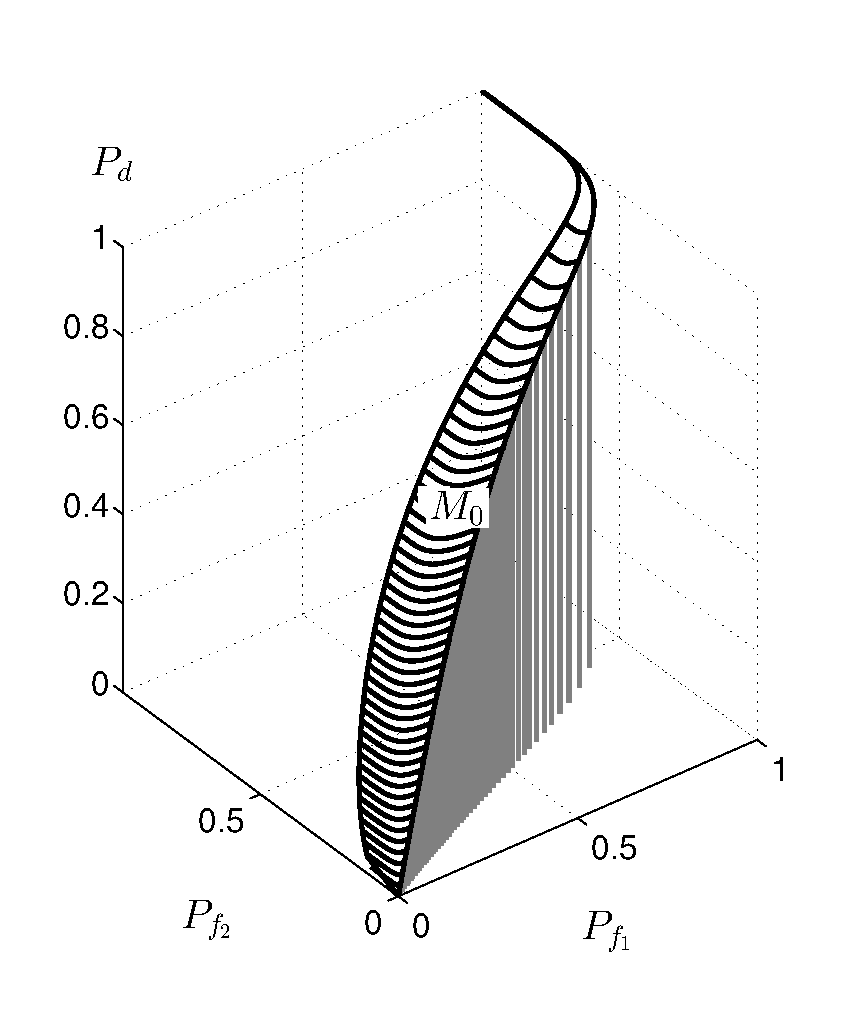
\includegraphics[width=12cm, height=16cm]{3/singleROC.eps}
\caption{Region that can be achieved by Neyman Pearson testing with $k_i \geq 0 (i=1, ..., M)$.}
\label{pic: surface for m0 gaussian}
\end{figure}

\begin{figure}[!t]
\centering
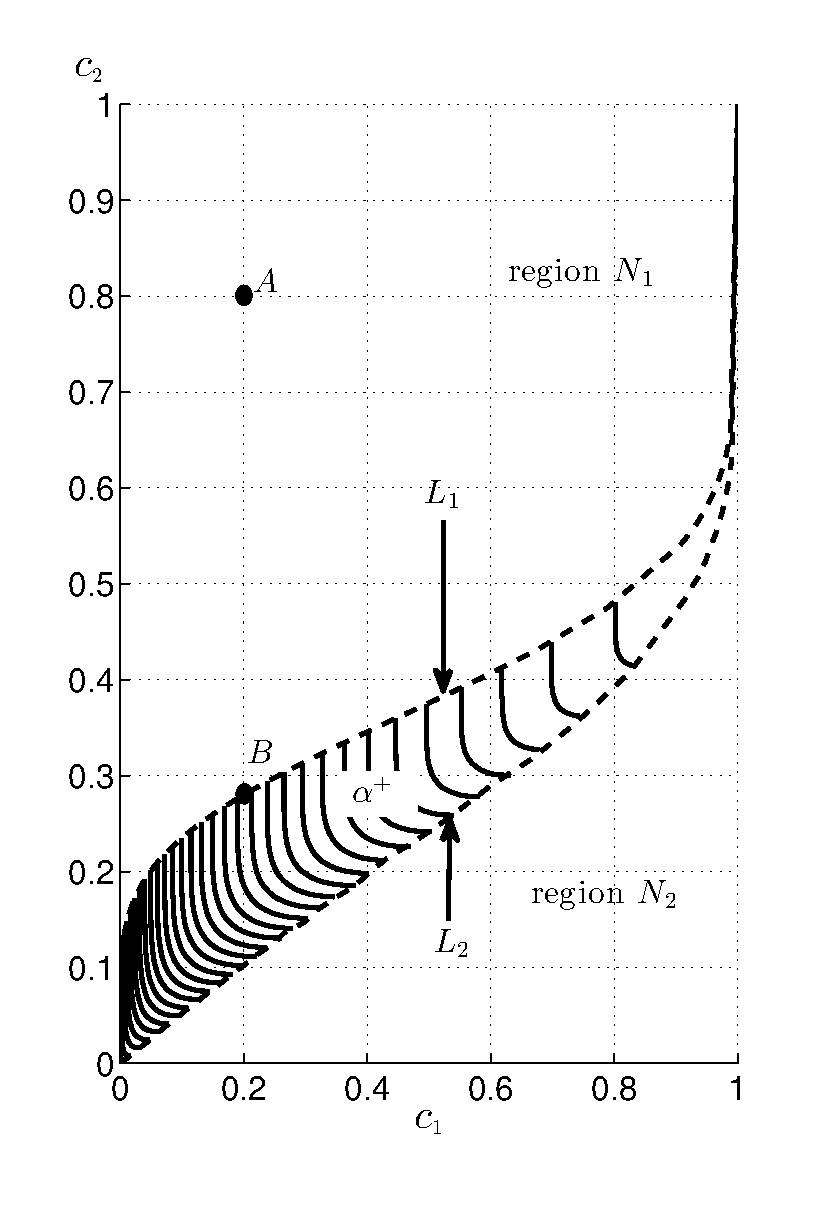
\includegraphics[width=12cm, height = 16cm]{3/singlecontour.eps}
\caption{Region that can be achieved by Neyman Pearson testing with $k_i \geq 0 (i=1, ..., M)$.}
\label{pic: contour for m0 gaussian}
\end{figure}

\begin{figure}[!t]
\centering
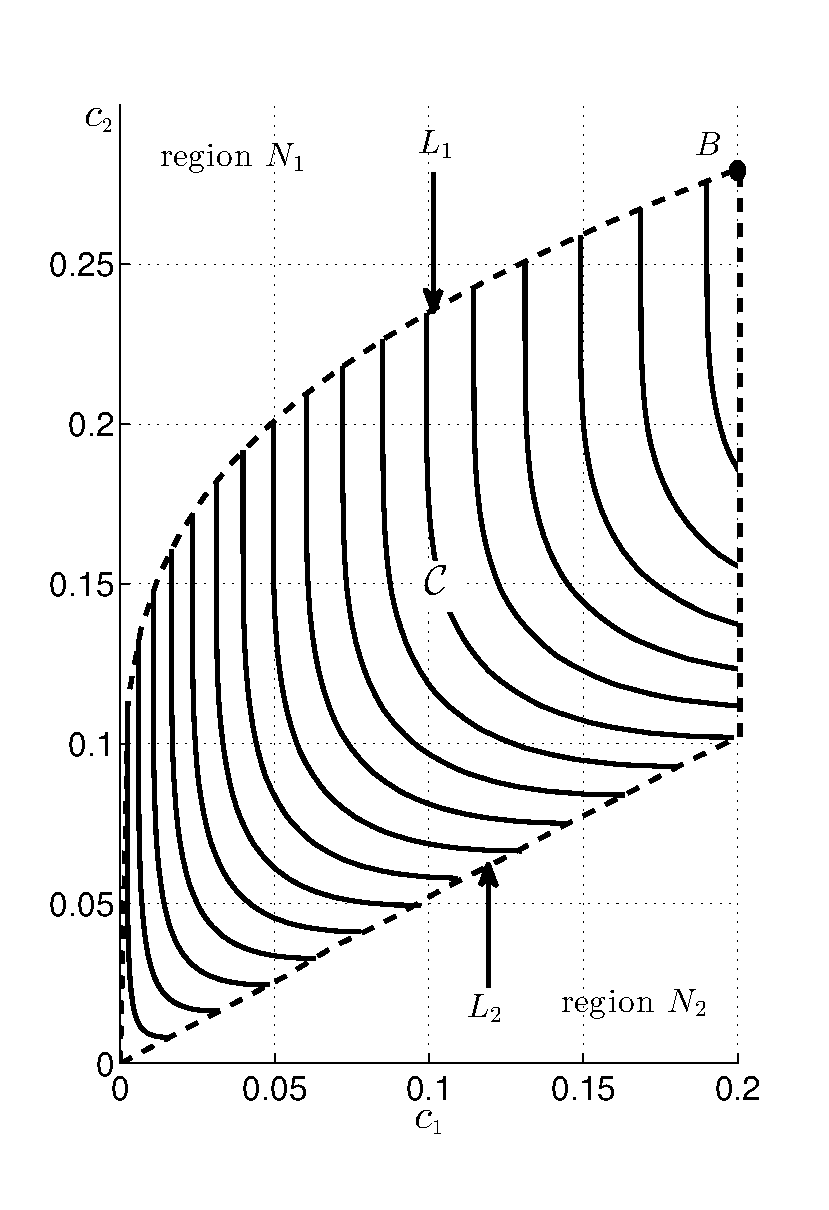
\includegraphics[width=12cm, height = 16cm]{3/singlecontour2.eps}
\caption{The region $\mathcal{C}$ when $c_1 = 0.2$ and $c_2 = 0.8$.}
\label{pic: regionC}
\end{figure}

Define curve $L_1$ as the set of points 
\[
\{ (c_1, c_2) \in L_1 | (c_1, c_2) \in \alpha^+ \;\;\text{and} \;\;(c_1, c_2+\epsilon)\notin \alpha^+ \;\;\;\;\text{for any positive $\epsilon$} \}\,.
\]
Define curve $L_2$ as the set of points 

\[
\{ (c_1, c_2) \in L_2 | (c_1, c_2) \in \alpha^+ \;\;\text{and} \;\;(c_1 + \epsilon, c_2)\notin \alpha^+ \;\;\;\;\text{for any positive $\epsilon$} \}\,.
\]
Let $N_1$ denote the region enclosed by line $c_1 = 0$, $c_2$; line $c_1$, $c_2 = 1$ and curve $L_1$.
Let $N_2$ denote the region enclosed by line $c_1 = 1$, $c_2$; line $c_1$, $c_2 = 0$ and curve $L_2$.
The regions $\alpha^+$, $N_1$ and $N_2$ are shown in Figure \ref{pic: contour for m0 gaussian}.

In the following, we present the decision rule for points belong to regions $N_1$ or $N_2$.

\noindent \textbf{Property 2:}
\textit{\\(1) All points belonging to region $N_1$ or curve $L_1$, if they have the same $c_1$, they have the same decision rule and same $P_d$.
\\(2) All points belonging to region $N_2$ or curve $L_2$, if they have the same $c_2$, they have the same decision rule and same $P_d$.
}

\noindent \textbf{PROOF}
Recall $F(\mathbf{c})$ is defined as the largest $P_d$ that can be achieved under constraint $\mathbf{P}_f = \mathbf{c}$ and 
       $G(\mathbf{c})$ is defined as the largest $P_d$ can be achieved under constraint $\mathbf{P}_f \leq \mathbf{c}$.
Firstly we will show $F(\mathbf{c}) = G(\mathbf{c}) $ when $\mathbf{c} \in \alpha^+$.

According to the definition of $\alpha^+$, for a point $(c_1, c_2) \in \alpha^+$, there exists a decision rule 
\[
\delta:\;\;\;\;f_0(x) \substack{H_0 \\ \geq \\ < \\ \bar{H}_0} k_1f_1(x) + k_2f_2(x) \;\;\;\;(k_1, k_2 \geq 0)
\]
such that under decision rule $\delta$, we have 
\begin{equation}
\label{1125a3}
\mathbf{P}_{f}(\delta) = \mathbf{c}\,.
\end{equation}
From ENP Lemma (\rmnum{2}), we know 
\begin{equation}
\label{1125c1}
P_d(\delta) = F(\mathbf{c})\,.
\end{equation}
Since $k_1, k_2 \geq 0$, according to ENP Lemma (\rmnum{3}), $\delta$ also achieve the largest $P_d$ while keeping $\mathbf{P}_f \leq \mathbf{c}$, i.e. 
\begin{equation}
 P_d(\delta) =G(\mathbf{c}) 
\label{1125a2}
\end{equation}
From \eqref{1125c1} and \eqref{1125a2} we can see $F(\mathbf{c}) = G(\mathbf{c})$ for $\mathbf{c} \in \alpha^+$.
In Section 2.2.2,  we have shown $G(\mathbf{c})$ is a non-decreasing function for each variable of $\mathbf{c}$, hence it can be concluded that $F(\mathbf{c})$ is a non-decreasing function for each variable of $\mathbf{c}$ on set $\alpha^+$.

As it is shown in Figure \ref{pic: contour for m0 gaussian}, A is a point in region ${N}_1$ with coordinates $(c_1, c_2) = (c_{1_A}, c_{2_A})$. In the following we will derive its optimal decision rule through MENP test. By optimal decision rule, we mean   it achieves the largest $P_d$ while keeping $\mathbf{P}_f \leq \mathbf{c}$.  
As point A does not belong to $\alpha^+$, we should use MNEP (\rmnum{2}) to get its decision rule. To do it, the first step is to determine set $\mathcal{C}$, which is the intersection of $\mathcal{A}_c$ and $\alpha^+$. In this case, set $\mathcal{C}$ is plotted in Figure \ref{pic: regionC}.
After we have $\mathcal{C}$, we need to find $\mathbf{c}^0 \in \mathcal{C}$ such that it maximum $F(\mathbf{c})$ among all $\mathbf{c} \in \mathcal{C}$.
Figure \ref{pic: contour for m0 gaussian} and Figure \ref{pic: regionC} shows that point B (with coordinate $(c_{1_B}, c_{2_B})$ where $c_{1_B} = c_{1_A}$) has the largest $c_1$ $c_2$ components among all $\mathbf{c} \in \mathcal{C}$. Since $F(\mathbf{c})$ is a non-decreasing function for $c_1$ and $c_2$ on set $\alpha^+$, it is easy to see
\begin{equation}
  \max_{\mathbf{c} \in \mathcal{C}}\;\;\;\;F(\mathbf{c}) = F(c_{1_B}, c_{2_B})\,.
  \label{2015apr30a0}
\end{equation}
 As point B is in set $\mathcal{C}$, there exists decision rule
 \[
\delta^\ast:\;\;\;\;f_0(x) \substack{H_0 \\ \geq \\ < \\ \bar{H}_0} k_1^\ast f_1(x) + k_2^\ast f_2(x) \;\;\;\;(k_1^\ast, k_2^\ast \geq 0)
 \]
 such that under $\delta^\ast$ we have  $P_{f_1}(\delta^\ast) = c_{1_B}$ and  $P_{f_2}(\delta^\ast) = c_{2_B}$. 
 From ENP (\rmnum{3}), it is easy to see $\delta^\ast$ is the optimal decision rule for point B.
 Since point B satisfies \eqref{2015apr30a0}, by using MENP (\rmnum{2}), we know $\delta^\ast$ is also the optimal decision rule for point A. Thus we can see the optimal decision rule for point A and point B are the same. Since point A lies in region $N_1$, point B lies in region $L_1$ and $c_{1_A} = c_{1_B}$, we can conclude for two points respectively belongs to $N_1$ and $L_1$, if they have the same $c_1$ component, they have the same decision rule and same $P_d$. 

Furthermore, we can see as long as A is in region $N_1$ its decision rule only depends on the value of $c_{1}$.  In other words, as long as A is in region $N_1$, with $c_1 = c_{1_A}$ fixed,  when $c_{2}$ changes, its optimal decision rule and $P_d$ remain the same. Hence we can conclude all points belonging to region $N_1$ or curve $L_1$, if they have the same $c_1$, they have the same decision rule and same $P_d$.

In the same way, we can prove: For points belong to region $N_2$ or curve $L_2$, if they have the same $c_2$ value, they have the same decision rule and same $P_d$.

Q.E.D

Since we have computed $P_d$ for $(c_1, c_2) \in N_0$ and curves $L_1$ and $L_2$ belong to $N_0$, we can get $P_d$ for $(c_1, c_2)$ belongs to $N_1$ or $N_2$ through \textbf{Property 2}. M-ROC surface for this example is given in Figure  \ref{pic: LJS}.
The whole M-ROC is divided into three regions ($M_1$, $M_0$ and $M_2$) to simplify our analysis. In region $M_1$, $P_d$ increases if and only if the value of $c_1$ increases, the value of $c_2$ does not affect $P_d$. On the opposite, in region $M_2$, $P_d$ increases if and only if the value of $c_1$ increases, it does not change with $c_2$. In region $M_0$, when one of $c_1$ or $c_2$ increases, $P_d$ will increase. In all these three regions, $P_d$ is non-decreasing with respect to $c_1$ and $c_2$. 

Next we discuss the different between the ENP test and MENP test concerning this example. 
From Figure \ref{pic: surface for m0 gaussian}, we can see the ENP test works only when the given $(c_1, c_2)$ belongs to set $\alpha^+$. For the case when $(c_1, c_2) \notin \alpha^+$, it cannot provide a solution.  However,  from Figure \ref{pic: LJS}, it can be seen by using the MENP test, we can get the decision rule for all $(c_1, c_2)$. 
In other words, the achievable region of the MENP test is larger than that of the ENP test. 
Besides that, we can see when $(c_1, c_2) \in \alpha^+$, the ENP test and the MENP test provides the same $P_d$. This results from the repetition between the two framework.  
\begin{figure}[!t]
\centering
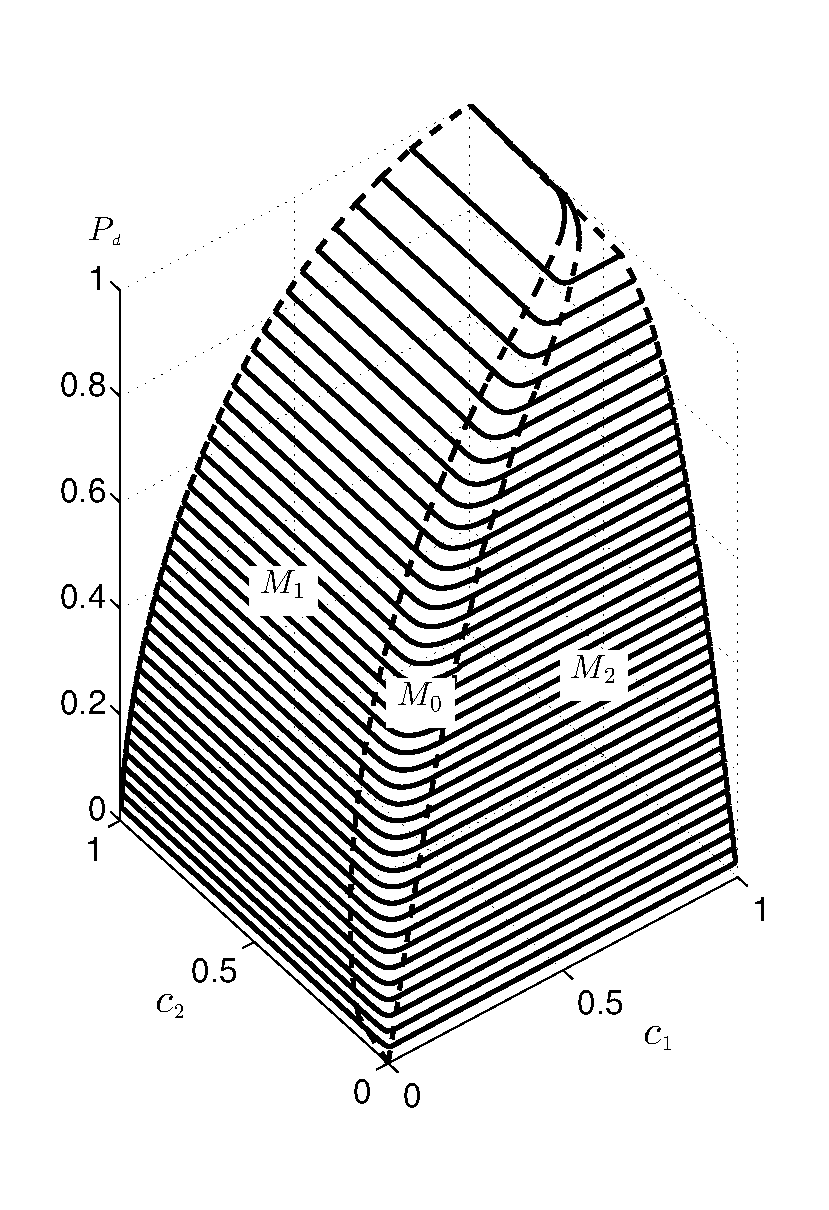
\includegraphics[width=12cm, height=16cm]{3/ROC2.eps}
\caption{The M-ROC surface for Gaussian Hypotheses.}
\label{pic: LJS}
\end{figure}

\noindent \textbf{Example 2:}

Next we consider a more general case of $M+1$ hypotheses given by 
\begin{equation}
\label{equ: m+1 Gaussian Hypo}
\begin{split}
H_0:\;\;\;\;\;\;&X\sim \mathcal{N}(\mu_0, \sigma_0^2)\\
H_1:\;\;\;\;\;\;&X\sim \mathcal{N}(\mu_1, \sigma_1^2)\\
  ......\\
H_M:\;\;\;\;\;\;&X\sim \mathcal{N}(\mu_M, \sigma_M^2)
\end{split}
\end{equation}
We will show when $\sigma_0^2 = \sigma_1^2 = ... = \sigma_M^2$ and $\mu_0 < \mu_i (i = 1, ..., M)$, the region achieved by ENP test with $k_i \geq 0 (i = 1, ..., M)$ degenerates to a curve.

Consider
\begin{equation}
\label{equ: define gx}
g(x) = \sum_{i=1}^{M}k_i\frac{f_i(x)}{f_0(x)}.
\end{equation}
Since 
\begin{equation}
\label{equ: gaussian PDF}
f_i(x) = \frac{1}{\sqrt{2\pi\sigma_i^2}}\exp(-\frac{(x-\mu_i)^2}{2\sigma_i^2}).
\end{equation}
we have
\begin{equation}
\label{g00}
g(x) = \sum_{i=1}^{M}k_i\frac{\frac{1}{\sqrt{2\pi\sigma_i^2}}\exp(-\frac{(x-\mu_i)^2}{2\sigma_i^2})}{\frac{1}{\sqrt{2\pi\sigma_0^2}}\exp(-\frac{(x-\mu_0)^2}{2\sigma_0^2})}
\end{equation}
Substitute  $\sigma_i^2 = \sigma_0^2 (i = 1, ..., M)$ into \eqref{g00}, we have 
\begin{equation}
\label{equ: gx cc}
g(x) = \sum_{i=1}^{M}k_i\exp(\frac{(\mu_i - \mu_0)(2x-\mu_i - \mu_0)}{2\sigma_0^2})
\end{equation}
Defining $p_i = \frac{\mu_i - \mu_0}{2\sigma_0^2}$, \eqref{equ: gx cc} can be written as
\begin{equation}
g(x) = \sum_{i=1}^{M}k_i\exp(p_i(2x-\mu_0 - \mu_i)
\end{equation}
From the condition $\mu_0 < \mu_i (i=1, ..., M)$, we can see $p_i >0$ and  $g(x)$ is a monotonically increasing function with $x$. Here from \textbf{Property 1} we know that $M_0$ (the region achieved by the ENP test with $k_i \geq 0 (i=1, ..., M)$) degenerates to a curve. Moreover, for a specific $\mathbf{c}$, the decision rule is 
\[
x \substack{H_0 \\ \leq \\ > \\ \bar{H}_0} x_0
\]
where $x_0 = \min\{F_1^{-1}(c_1), ..., F_M^{-1}(c_M)\}$. The associated probability of detection is
\[
P_d = F_0(x_0)
\]

Figure \ref{pic: surface for same variance} shows the M-ROC surface for $M=2$, $\mu_0 = 0$, $\mu_1 = 1$, $\mu_2 = 2$ and $\sigma_0^2 = \sigma_1^2 = \sigma_2^2 = 1$. The bold curve is region $M_0$.
To simplify the analysis, the whole M-ROC surface is devided into 3 regions ($M_1$, $M_0$ and $M_2$) as it is shown in Figure \ref{pic: surface for same variance}.  In region $M_1$, $P_d$ increases if and only if the value of $c_1$ increases, the value of $c_2$ does not affect $P_d$. On the opposite, in region $M_2$, $P_d$ increases if and only if the value of $c_1$ increases, it does not change with $c_2$. In region $M_0$, $P_d$ increases if and only if both $c_1$ and $c_2$ increase (This is different from Example 1, because in this case, region $M_0$ degenerates to a curve). 
In all these three regions, $P_d$ is non-decreasing with respect to $c_1$ and $c_2$. 

From the definition of $M_0$, we know $M_0$ is the region can also be achieved by both ENP test and MENP test. We can see, comparing to the ENP test, the MENP test has a much larger achievable region (the MENP test can achieve the $P_d$ for the whole $c_1-c_2$ plane, while the ENP test can only achieve the $P_d$ when $(c_1, c_2)$ lies in $\alpha^+$, which is also a curve because $\alpha^+$ is the projection of $M_0$). 

\begin{figure}[!t]
\centering
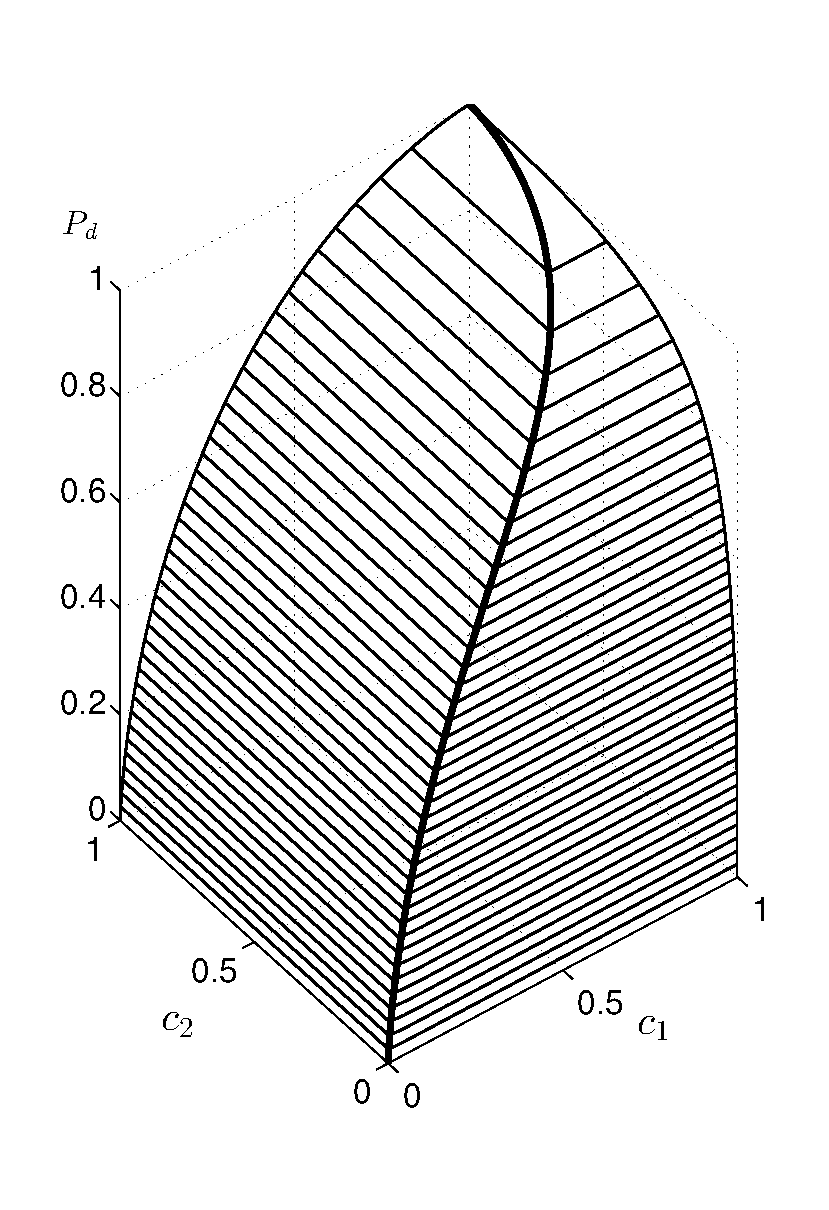
\includegraphics[width=12cm, height=16cm]{3/gaussian.eps}
\caption{The M-ROC for Gaussian distribution with same variance.}
\label{pic: surface for same variance}
\end{figure}


%==================================================================================================
  \typeout{}
  % Chi-Square Case
\subsection{MROC Surface under Chi-Square Hypotheses}
\noindent\textbf{Example:}

Assume $M+1$ hypotheses  given as:
\begin{equation}
  \label{equ: Chisquare Hypothesis}
  \begin{split}
    H_0:\;\;\;\;\;\;\;\;&\frac{X}{\sigma_0^2} \sim \mathcal{X}^2(2N)\\
    H_1:\;\;\;\;\;\;\;\;&\frac{X}{\sigma_1^2} \sim \mathcal{X}^2(2N)\\
    &......\\
    H_M:\;\;\;\;\;\;\;\;&\frac{X}{\sigma_2^M} \sim \mathcal{X}^2(2N)\,,
  \end{split}
\end{equation}
where $\mathcal{X}^2(2N)$ is the Chi-square distribution with  $2N$ degree freedom($N$ is an integer, $\sigma_0^2 < \sigma_1^2, ..., \sigma_M^2$ and $\sigma_i^2 \neq \sigma_j^2$ if $i \neq j$). By a random variable transformation space \cite{mark2011probability}, we can get the PDFs for the hypotheses:

\def \CHISQU[#1]{\frac{1}{#1 2^N\Gamma(N)}\left(\frac{x}{#1}\right)^{N-1}\exp\left(-\frac{x}{2#1}\right)\\}
\begin{equation}
  \label{equ: Chisquare Distribution}
  \begin{split}
    H_0:\;\;\;\;\;\;\;\;&f_0(x) = \CHISQU[\sigma_0^2]\\
    H_1:\;\;\;\;\;\;\;\;&f_1(x) = \CHISQU[\sigma_1^2]\\
    &......\\
    H_M:\;\;\;\;\;\;\;\;&f_2(x) = \CHISQU[\sigma_M^2]\,.
  \end{split}
\end{equation}

In the following, we will prove that in this example the region achieved by ENP test with $\mathbf{k}$ degenerates to a curve.

Consider
\begin{equation}
\label{equ: decision rule chi}
  g(x) = \frac{\sum_{i=1}^{M}k_if_i(x)}{f_0(x)} \;\;\;\;k_i \geq 0
\end{equation}
Substituting $f_i(x) (i=1, ..., M)$ from \eqref{equ: Chisquare Distribution} into \eqref{equ: decision rule chi}, we get:

\begin{equation}
  \label{equ: decision rule chi 1}
g(x) = \sum_{i=1}^{M}k_i'\exp{(\frac{1}{2\sigma_0^2} - \frac{1}{2\sigma_i^2})x} 
\end{equation}
where $k_i' = k_i(\frac{\sigma_0}{\sigma_i})^{2N}, i= 1, ..., M$. Define $p_i = \frac{1}{2\sigma_0^2} - \frac{1}{2\sigma_i^2}, i=1, ..., M$. Hence $g(x) =  \sum_{i=1}^{M}k_i'\exp{(p_ix)}$.

The parameters $k_i' (i=1, ..., M)$ are always non-negative when $k_i (i=1, ..., M)$ are such, and from 
 the condition $\sigma_0^2 \leq \sigma_i^2 (i=1, ..., M)$ we can conclude $p_i (i=1, ..., M)$ are positive. Hence $g(x)$ is a monotonically increasing function with $x$. From \textbf{Property 1}, we have that the region achieved by ENP test with $k_i (i = 1, ..., M)$ degenerates to a curve. For a specific $\mathbf{c}$, the decision rule is
\begin{equation}
  \label{equ: decision rule chi 2}
  x \substack{\bar{H}_0 \\ \geq \\ < \\ H_0} x_0\,,
\end{equation}
where $x_0 = \min\{F_1^{-1}(c_1), ..., F_M^{-1}(c_M)\}$,
and the corresponding $P_d = F_0(x_0)$. 

Figure \ref{pic: LJS for chisquare} shows the M-ROC surface for $M=2$, $\sigma_0^2 = 1$, $\sigma_1^2 = 1.1$, $\sigma_2^2 = 1.15$ and $N=120$. The bold curve  is the region $M_0$. 

\begin{figure}[!t]
\centering
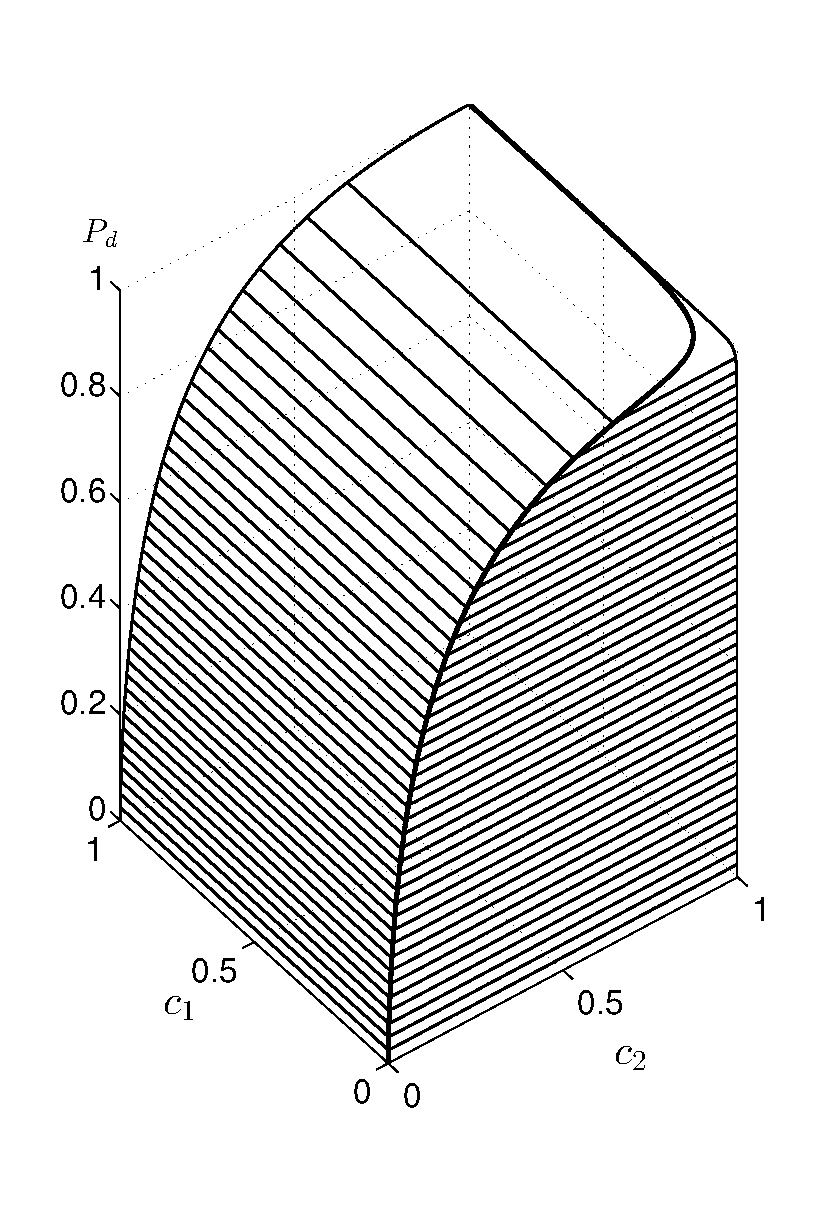
\includegraphics[width=12cm, height=16cm]{3/example3.eps}
\caption{The M-ROC for the Chi-square example.}
\label{pic: LJS for chisquare}
\end{figure}



%==========
\typeout{}
% This is the chapter for applying MENP framework to spectrum sensing.
\chapter{Application of MENP Framework in Spectrum Sensing and Simulation Results}
Upon examination of the theoretical part of MENP framework and M-ROC, this thesis will now apply the new hypotheses testing framework to application, which in our case is spectrum sensing for multiple primary users. We proposed energy based detector and cyclostationary based detector to detect multiple OFDM signals under AWGN channel. Performance analysis results, which illustrate the performance of both detector, will be presented. 
%----------------------------------------------------------------------------------------------

\typeout{}
% Energy based spectrum sensing
\section{Energy based Spectrum Detector for Multiple Primary Users}
\subsection{System Model}
We consider a cognitive radio system where the licensed frequency spectrum could be occupied by one of two distinct signals $\{s_A, s_B\}$ or it could be vacant. Let $H_0$ denote the hypothesis under which the channel is free, ${H}_1$ denote the hypothesis under which the channel is occupied by $s_A$ and ${H}_2$ denote the hypothesis under which the channel is occupied by $s_B$. We are interested to test $H_0$ against $\bar{{H}_0}$, where $\bar{H}_0$ denotes the hypothesis under which the channel is not free, using MENP framework.

A block diagram of the system is illustrated in Figure \ref{pic: block diagram}.

\begin{figure}[!hbp]
\centering
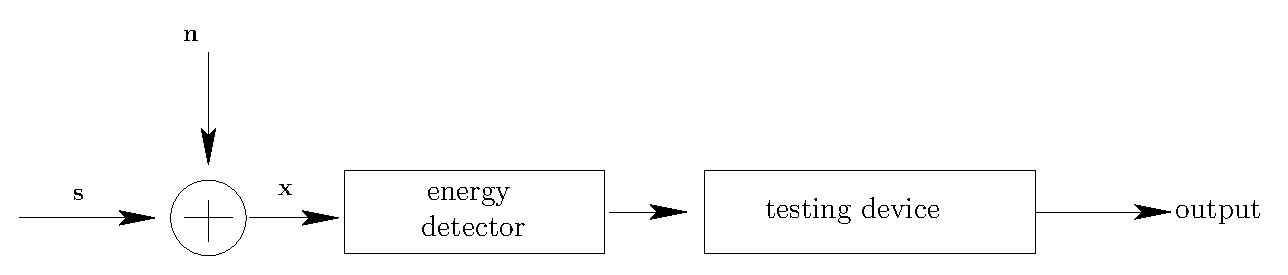
\includegraphics[width = \textwidth]{4/fig4.eps}
\caption{Block Diagram for Spectrum Sensing}
\label{pic: block diagram}
\end{figure}

The detector consists of a measuring device followed by a testing device. 
The measuring device observes the noisy version of the received signals and forms the energy of their sampled version.
With this energy, the testing device employs the MENP framework to decide about the state of the channel.
The input to the measuring device is 
\begin{equation}
  \mathbf{x} = \begin{cases}
	\mathbf{n}\;\;\;\;\;\;&\text{when $H_0$ is true}\\
	\mathbf{n}+\mathbf{s}_A\;\;\;\;\;\;&\text{when $H_1$ is true}\\
	\mathbf{n}+\mathbf{s}_B\;\;\;\;\;\;&\text{when $H_2$ is true}\\
  \end{cases}
  \label{equ:1222n0}
\end{equation}
where 
\begin{equation}
  \begin{cases}
	&\mathbf{x} = (x_0, x_1, \cdots, x_{N-1})\\
	&\mathbf{s}_A = (s_{A0}, s_{A1}, \cdots, s_{A(N-1)})\\
	&\mathbf{s}_B = (s_{B0}, s_{B1}, \cdots, s_{B(N-1)})\\
	&\mathbf{n} = (n_{0}, n_{1}, \cdots, n_{N-1})\,.
  \end{cases}
  \label{1222n1}
\end{equation}

We assume  $s_{A_i}$ $s_{B_i}$ and $n_i$ are zero-mean independent and identically distributed (iid) circularly symmetric complex Gaussian (CSCG) random variables with variances $2\sigma_{s_A}^2$, $2\sigma_{s_B}^2$ and $2\sigma_{n}^2$, i.e., $s_{A_i} \sim \mathcal{CN}(0, 2\sigma_{s_A}^2)$, $s_{B_i} \sim \mathcal{CN}(0, 2\sigma_{s_B}^2)$ and $n_i \sim \mathcal{CN}(0, 2\sigma_{n}^2)$.
Each noisy sample $x_i = s_i + n_i$ is governed by a probability law under each hypothesis. In our model
since the noise and signal are independent, $s_i+ n_i \sim \mathcal{CN}(0, 2(\sigma_{s}^2 + \sigma_n^2))$.  Define $\sigma_0^2 = \sigma_n^2$, $\sigma_1^2 = \sigma_{s_A}^2 + \sigma_n^2$ and $\sigma_2^2 = \sigma_{s_B}^2 + \sigma_n^2$, we can see
\begin{equation}
  \label{1129a1}
  \begin{split}
  n_i &\sim \mathcal{CN}(0, 2\sigma_0^2)\\
  n_i + s_{A_i} &\sim \mathcal{CN}(0, 2\sigma_1^2)\\
   n_i + s_{B_i}&\sim \mathcal{CN}(0, 2\sigma_2^2) \,,
  \end{split}
\end{equation}
thus the distribution of $x_i$ under each hypothesis is given by
\begin{equation}
   \begin{split}
  H_0:\;\;\;\;\begin{pmatrix} x_{i_R} \\ x_{i_I} \end{pmatrix} \sim \mathcal{N}\Big( \begin{bmatrix} 0 \\ 0 \end{bmatrix}, \begin{bmatrix} \sigma_0^2 & 0\\ 0 & \sigma_0^2 \end{bmatrix} \Big)\\
  H_1:\;\;\;\;\begin{pmatrix} x_{i_R} \\ x_{i_I} \end{pmatrix} \sim \mathcal{N}\Big( \begin{bmatrix} 0 \\ 0 \end{bmatrix}, \begin{bmatrix} \sigma_1^2 & 0\\ 0 & \sigma_1^2 \end{bmatrix} \Big)\\
  H_2:\;\;\;\;\begin{pmatrix} x_{i_R} \\ x_{i_I} \end{pmatrix} \sim \mathcal{N}\Big( \begin{bmatrix} 0 \\ 0 \end{bmatrix}, \begin{bmatrix} \sigma_2^2 & 0\\ 0 & \sigma_2^2 \end{bmatrix} \Big)
\end{split}
  \label{equ:xdistribution}
\end{equation}
where $x_{i_R}$ and $x_{i_I}$ are real and imaginary components of $x_i$.
In our case, the measuring device is an energy detector, with output 
\begin{equation} 
  Y = \sum_{i=0}^{N-1}|x_i|^2 = \sum_{i=0}^{N-1}(x_{i_R}^2+x_{i_I}^2)\,.
  \label{equ: testing device}
\end{equation}
By observing $y$, a realization of $Y$, the testing device determines the status of the channel. 
Since $x_{i_R}, x_{i_I}$ are uncorrelated Gaussian random variable with zero mean and variance $\sigma_i^2$, $\frac{y}{\sigma_i^2} = \sum_{n=0}^{N-1}((\frac{x_{i_R}}{\sigma_i})^2 + (\frac{x_{I_i}}{\sigma_i})^2)$ is governed by a Chi-Square distribution with $2N$ degree of freedom under hypothesis $H_i$.
Hence the distribution of $Y$ can be expressed as:
\begin{equation} 
  \label{equ: abstract}
  \begin{split}
	H_0:\;\;\;\;&\frac{Y}{\sigma_0^2}\sim \mathcal{X}(2N)\\
	H_1:\;\;\;\;&\frac{Y}{\sigma_1^2}\sim \mathcal{X}(2N)\\
	H_2:\;\;\;\;&\frac{Y}{\sigma_2^2}\sim \mathcal{X}(2N)\,,
  \end{split}
\end{equation}
where $\mathcal{X}(2N)$ is the Chi-square distribution with $2N$ degrees of freedom. 

Let $P_d$ denote the probability of detection, i.e. the probability that the channel is correctly declared vacant ($H_0$ is correctly declared true) and $P_{f_1}$ $P_{f_2}$ denote the probability of false alarm with respect to $s_A$  and $s_B$, i.e. the probability that the channel is declared vacant when signal $s_A$ ($s_B$) is present. Let $c_i$ ($i = 1, 2$) denotes the specific positive constraints on the probability of false alarm. The performance of the system can be depicted by $P_d$ and $c_i$ ($i = 1, 2$), and we use the MENP framework to solve following optimization problem:
\begin{equation}
  \begin{split}
	\max\;\;\;\;&P_d\\
	\text{s.t.}\;\;\;\;&P_{f_1}\leq c_1\\
	&P_{f_2} \leq c_2\,.
  \end{split}
  \label{1129a3}
\end{equation}
Our goal is to plot M-ROC surface and to find the decision rule for a given $c_1, c_2$ value.

\subsection{Numerical Results}
Assume $\sigma_n^2=0.1$ $\sigma_{s_A}^2=0.05$ $\sigma_{s_B}^2=0.1$ and $N=20$. We can see $\sigma_0^2=0.1$ $\sigma_1^2=0.15$ and $\sigma_2^2=0.25$, 
thus $\sigma_0^2 < \sigma_1^2, \sigma_2^2$. Hence the problem given in \eqref{1129a3} for hypotheses \eqref{equ: abstract} has the same form as that of Chi-Square Example given in chapter 3. 
If $y$ is an observation of $Y$, 
from the conclusion in chapter 3 the optimal  decision rule for a given $c_1, c_2$ is 
\begin{equation}
  y \substack{H_0 \\ < \\ > \\ \bar{H}_0} V_\tau
  \label{equ:1129a4}
\end{equation}
where 
\begin{equation}
  V_\tau = \min\{F_1^{-1}(c_1),  F_2^{-1}(c_2)\}
  \label{equ:2015may1a2}
\end{equation}
and function $F_1,  F_2$ are the CDFs of $Y$ under hypothesis $H_1, H_2$ respectively. The expression of $P_d$ is 
\begin{equation}
  P_d = F_0(V_\tau)\,.
  \label{equ:1129a5}
\end{equation}

Similar to energy detection in binary hypothesis testing, energy detection for multiple hypothesis testing differentiates between $H_0$ and $\bar{H}_0$ by comparing the test statistic (in form of energy) with a threshold $V_\tau$. The value of the threshold can be determined by the probability of false alarm constraints.   

We use Matlab to compute the M-ROC for this energy detector. The value of $c_1, c_2$ range from $0.0001$ to $0.2$ with step $0.0001$. By using \eqref{equ:1129a4} \eqref{equ:2015may1a2} and \eqref{equ:1129a5}, the value of $P_d$ can be acquired. The M-ROC is illustrate in Figure. \ref{pic:1201a1}. The bold curve in the middle is region $M_0$ ($M_0$ is defined in section 3.1). 

In the context of spectrum sensing, for a given $c_1, c_2$, it means: for primary user $s_A$ (or $s_B$), the probability of being interfered by secondary user is less than $c_1$ (or $c_2$). Hence we can see, when designing the spectrum sensing system,  $c_1, c_2$ can be used to measure how much of protection that the system can provide to primary user $s_A$ and $s_B$.  The lower $c_1$ ($c_2$) is, the more protection the system can provide to primary user $s_A$ ($s_B$). $P_d$ can be used to describe the system's ability of detecting a free channel.   First we can observe from Figure \ref{pic:1201a1} that for any $c_1, c_2$ the system provides an associated $P_d$ and $P_d$ is non-decreasing with respect to $c_1$ and $c_2$. This accords with intuitive and the theoretical proof in section 2.2.     
Next we concern some specific points on the M-ROC surface. For $c_1 = 0.075$ and $c_2  = 0.1$, the largest $P_d$ can be achieved is $0.609$. And when $c_2$ decreases to $0.005$ and  $c_1$ remains the same, the $P_d$ does not change.   
 It means properly increasing the level to protection to one primary user (in this case, we increase the protection to primary user $s_B$ by decreasing $c_2$), the system's performance may not be jeopardized ($P_d$ does not decrease).  
Then consider the situation when $c_1 = 0.115$ and $c_2 = 0.100$. In such case, the associated $P_d$ is $0.711$. Now increase $c_2$ to $0.150$, we can see the associated $P_d$ is still $0.711$. We can see even though we decrease the protection to primary user $s_B$, the system's performance is not increased.  
This suggests blindly decreasing the level of protection to one primary user (by increasing the value of $c_1$ or $c_2$) may not help increasing the performance of the system (increasing $P_d$). To increase $P_d$, we should check the M-ROC surface to choose a proper $c_1$ and $c_2$ combination.

\begin{figure}[!t]
\centering
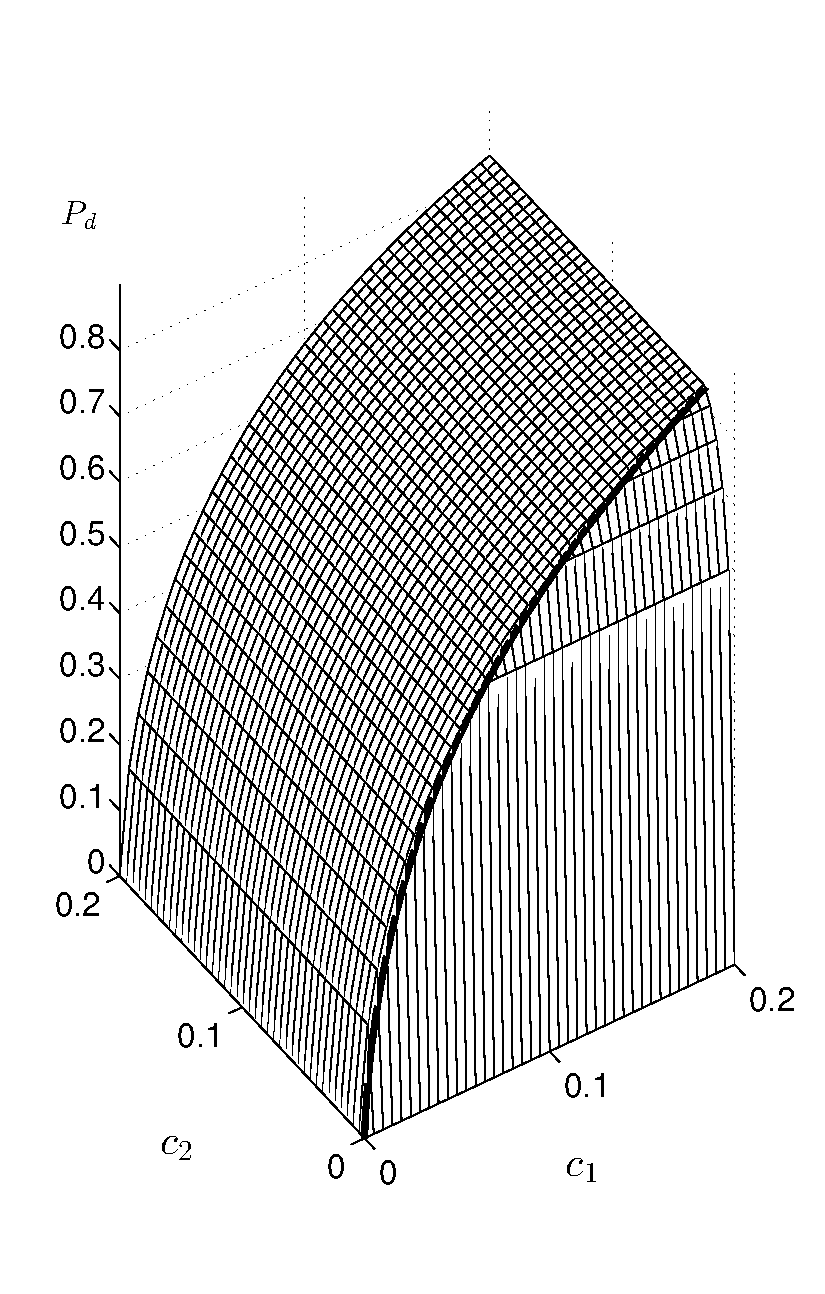
\includegraphics[width=12cm, height=16cm]{4/mathc1c2pd.eps}
\caption{M-ROC surface for $\sigma_n^2 = 0.1$, $\sigma_{s_A}^2=0.05$, $\sigma_{s_B}^2=0.15$ and $N = 20$.}
\label{pic:1201a1}
\end{figure}

\subsection{Simulation Results}
The simulation results presented in this thesis were obtained by using Monte Carlo techniques. All of Matlab code for the programs required to reproduce the simulation results are contained in the attached CD. Appendix B presents a brief tutorial on the uses of the various files for the simulation. The system model and parameters are the same with the numerical analysis.

The simulation presents the performance of energy detector when $c_1$ and $c_2$ separately increase from $0.005$ to $0.2$ with steps $0.005$. For a specified $c_1$ and $c_2$, we compute  its associated MENP decision rule, which is given by \eqref{equ:1129a4} and \eqref{equ:2015may1a2}. 

For each decision rule calculated through \eqref{equ:1129a4} and \eqref{equ:2015may1a2}, we use Monte Carlo simulation to get its associated $P_d$, $P_{f_1}$ and $P_{f_2}$.   
In order to ensure highly accurate results, a minimum of 600 events and 100000 experiments are required. The simulation result of the M-ROC surface is presented in Fig. \ref{pic:2015may1}. $P_d$ is acquired through simulation for each intersection of the mesh in Fig. \ref{pic:2015may1}, except for points $c_1 = 0$, $c_2$ and $c_2 = 0$, $c_1$, which are plotted to better illustrate the M-ROC surface. 
Compare Fig. \ref{pic:2015may1} with Fig. \ref{pic:1201a1}, we can see the simulation result accords with the numerical analysis, which verify our theoretical analysis.

Fig. \ref{pic:2015may1a0} depicts the relationship between  $P_d$ and $V_\tau$ for each $V_\tau$  computed through \eqref{equ:2015may1a2}.  For each $c_1, c_2$, the associated $(V_\tau, P_d)$ is plotted as `o'. The curve in Fig. \ref{pic:2015may1a1} is the theoretical relationship between $P_d$ and $V_\tau$ calculated through \eqref{equ:1129a5}. 
Since $c_1$ and $c_2$ are discrete, the value of $V_\tau$ is also discrete (as we can see from Fig. \ref{pic:2015may1a0}). Furthermore, for different $(c_1, c_2)$, the value of $V_\tau$ may be the same, 
e.g. for $(c_1, c_2) = (0.1, 0.1)$, the value of $V_\tau$ is $4.358$; for $(c_1, c_2) = (0.1, 0.2)$, we have $V_\tau = 4.358$.  
In our program, we use Monte Carlo simulations to acquire the $P_d$ for each $(c_1, c_2)$.  For  $(c_1, c_2) = (0.1, 0.1)$, the $P_d$ we acquired is $0.67819$; for $(c_1, c_2) = (0.1, 0.2)$, the $P_d$ we acquired through simulation is $0.67823$. There are some slight difference between the two $P_d$ (even though the decision rule are the same). This is because when the   experiments times is not unlimited, the simulation results could be different from the theoretical results. This explains why in Fig. \ref{pic:2015may1a0} for one $V_\tau$ value, there may be multiple $P_d$ corresponds with it.  
From Fig. \ref{pic:2015may1a0}, we can see the simulation result accords with the numerical analysis. 

Fig. \ref{pic:2015may1a1} depicts the relationship between $P_{f_1}$, $P_{f_2}$ and $P_d$ for each decision rule computed through \eqref{equ:2015may1a2}.  
For each $c_1, c_2$, the associated $(P_{f_1}, P_{f_2}, P_d) $ is plotted as `o'.
The curve in Fig. \ref{pic:2015may1a1} is the theoretical relationship between $P_{f_1}$ $P_{f_2}$ and $P_d$. This curve is computed through \eqref{equ: pd under x0}. 
As we have discussed, for one decision rule, there could be multiple simulation results for $(P_{f_1}, P_{f_2}, P_d)$, and these simulation results may be slight different due to the experiments times' limitation. 
This explains why in Fig. \ref{pic:2015may1a1} for some $(P_{f_1}, P_{f_2}, P_d)$ points, there are several  `o' around the theoretical curve.
By comparing the simulation results and the theoretical curve, we can see the simulation result accords with the numerical analysis. 


\begin{figure}[!t]
\centering
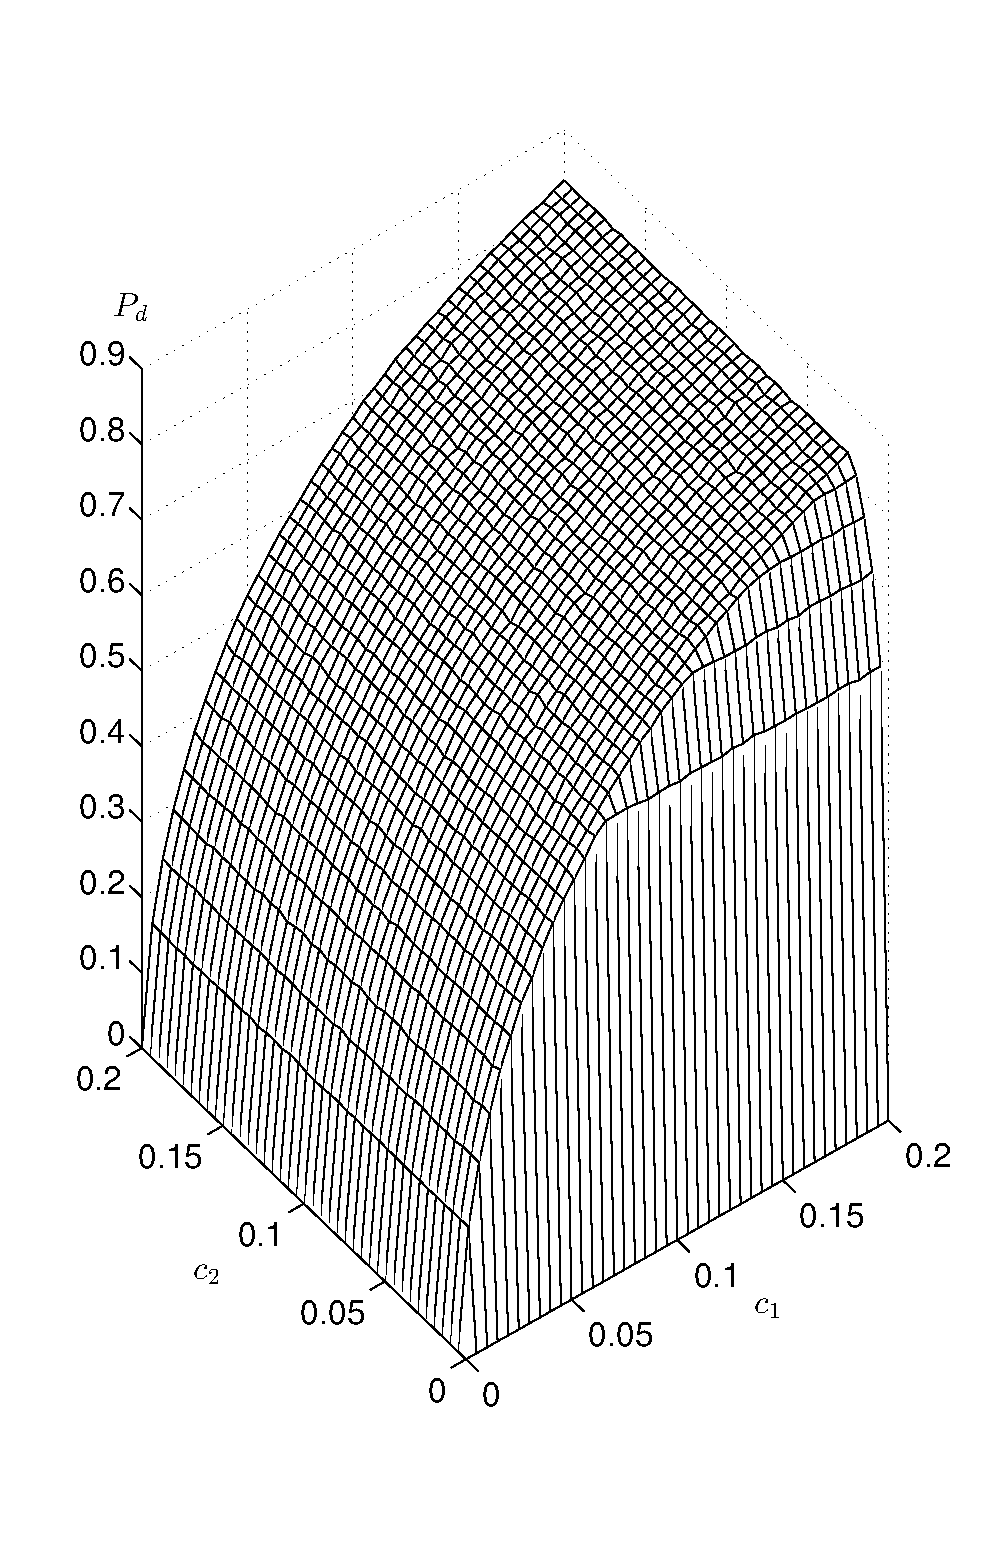
\includegraphics[width=12cm, height=16cm]{4/c1c2pd.eps}
\caption{Simulation results of M-ROC surface for $\sigma_n^2 = 0.1$, $\sigma_{s_A}^2=0.05$, $\sigma_{s_B}^2=0.15$ and $N = 20$.}
\label{pic:2015may1}
\end{figure}


\begin{figure}[!t]
\centering
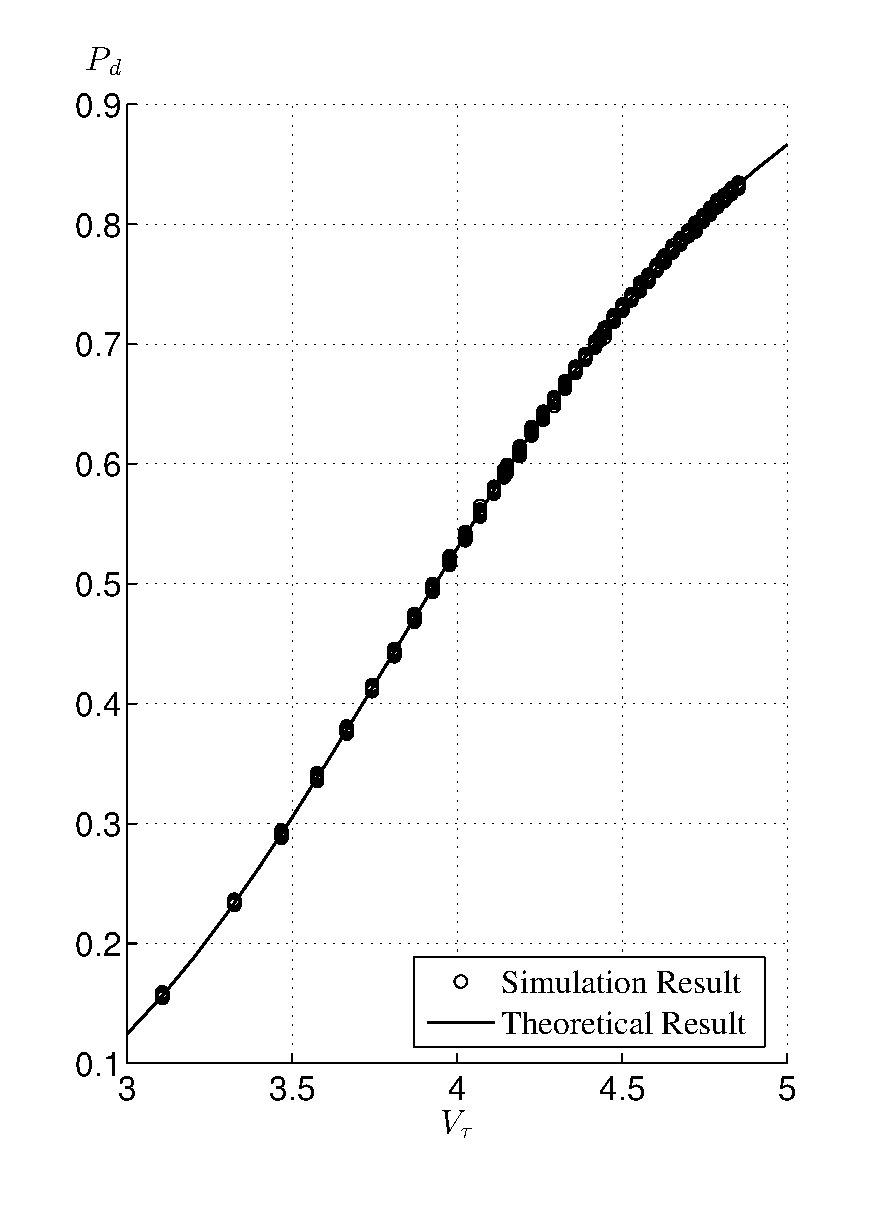
\includegraphics[width=12cm, height=16cm]{4/tpd.eps}
\caption{Relationship Between $V_\tau$ and its associated $P_d$.}
\label{pic:2015may1a0}
\end{figure}

\begin{figure}[!t]
\centering
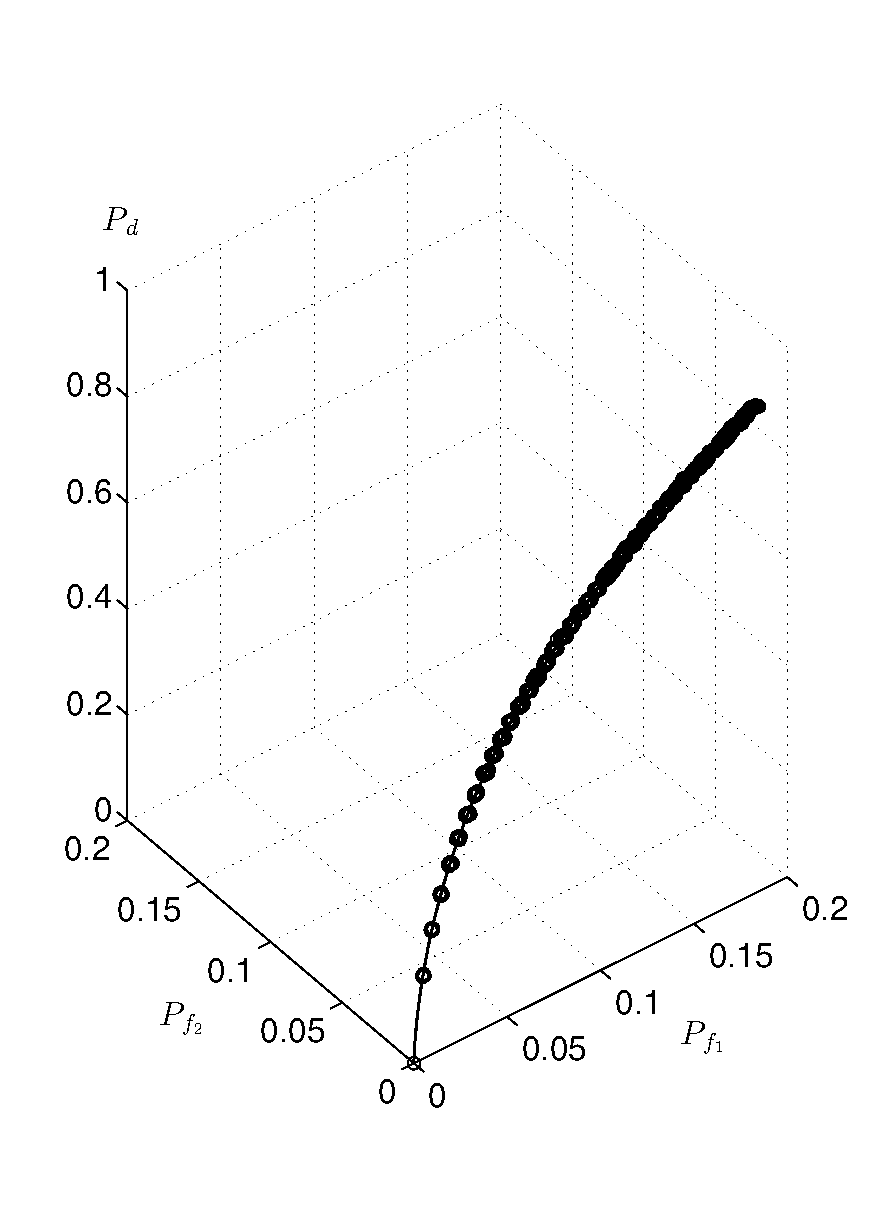
\includegraphics[width=12cm, height=16cm]{4/pdpf1pf2.eps}
\caption{Relationship between $P_{f_1}$, $P_{f_2}$ and $P_d$.}
\label{pic:2015may1a1}
\end{figure}



%----------------------------------------------------------------------------------------------


\typeout{}
% cyclostationary based energy detection
\section{Cyclostationary Detection for multiple Primary Users}
\subsection{System Model}

We consider a cognitive radio system where the spectrum can be occupied by exactly one of two distinct primary signals $\{s_A, s_B\}$ or it could be vacant. Let $H_0$ denote the situation under which the channel is free, $H_1$ denote the hypothesis under which the channel is occupied by signal $s_A$ and $H_2$ denote the hypothesis under which the channel is occupied by signals $s_B$. Both $s_A, s_B$ are OFDM signals with same frame structure. The block diagram of the system is illustrated in Figure.

\begin{figure}[!t]
  \centering 
  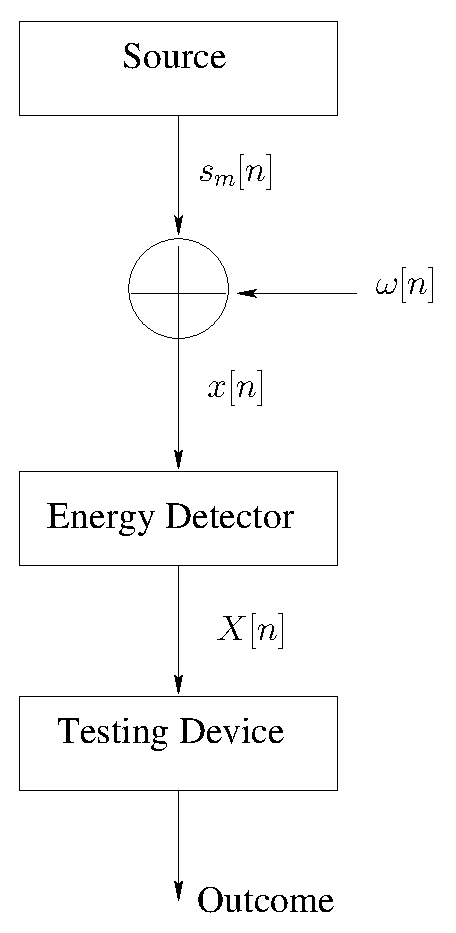
\includegraphics[width=\textwidth]{4/fig1.eps}
  \caption{Block Diagram for  cyclostationary detector.}
  \label{pic:1222a0}
\end{figure}
The measuring device observes $M$ samples of the noise version signals that could present in the channel and output a suitable testing statistics. With this statistics, the testing device employs MENP to determine the status of the channel. The input of measuring device is
\begin{equation}
  \mathbf{x} = \begin{cases}
	\mathbf{n}\;\;\;\;\;\;&\text{when $H_0$ is true}\\
	\mathbf{n}+\mathbf{s}_A\;\;\;\;\;\;&\text{when $H_1$ is true}\\
	\mathbf{n}+\mathbf{s}_B\;\;\;\;\;\;&\text{when $H_2$ is true}\\
  \end{cases}
  \label{equ:1209a1}
\end{equation}
where 
\begin{equation}
  \begin{cases}
	&\mathbf{x} = (x_0, x_1, \cdots, x_{M-1})\\
	&\mathbf{s}_A = (s_{A0}, s_{A1}, \cdots, s_{A(M-1)})\\
	&\mathbf{s}_B = (s_{B0}, s_{B1}, \cdots, s_{B(M-1)})\\
	&\mathbf{n} = (n_{0}, n_{1}, \cdots, n_{M-1})\,.
  \end{cases}
  \label{xssn}
\end{equation}
Assume each OFDM frame contains a CP sequence of length $l_C$ followed by a data sequence of length $l_D$, so the total length of an OFDM frame is $l_0 = l_C+l_D$. In general case, when there are signal transmitting, the receiver is not synchronized to the transmitted signal, i.e. $s_{A0}$ ( or $s_{B0}$) is not the first symbol of an OFDM frame. Let $\tau$ represents the synchronization mismatch. That is, when $\tau = 0$, $s_0$ is the first symbol of an OFDM frame; when $\tau = l_C+l_D -1$, $s_0$ is the last symbol of an OFDM frame. Let $M = Kl_0$, we can see when perfect synchronization the detector would observe $K$ complete  OFDM frames (as it is shown in Figure); otherwise, the detector would observe $K-1$ complete OFDM frames and $2$ incomplete OFDM frames (as it is shown in Figure). 
\begin{figure}[!t]
  \centering 
  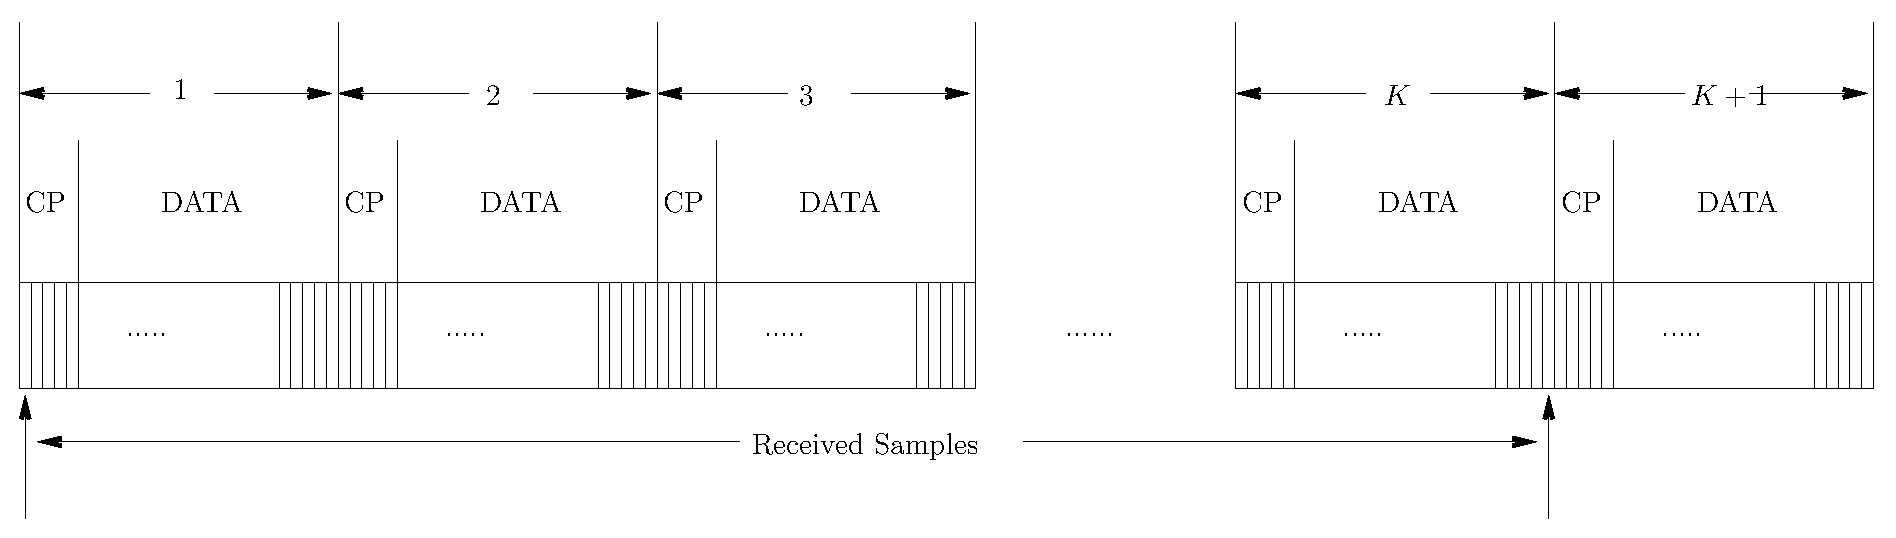
\includegraphics[width=\textwidth]{4/fig2.eps}
  \caption{Received signal for perfect synchronization.}
  \label{pic:1221n0}
\end{figure}

\begin{figure}[!t]
  \centering 
  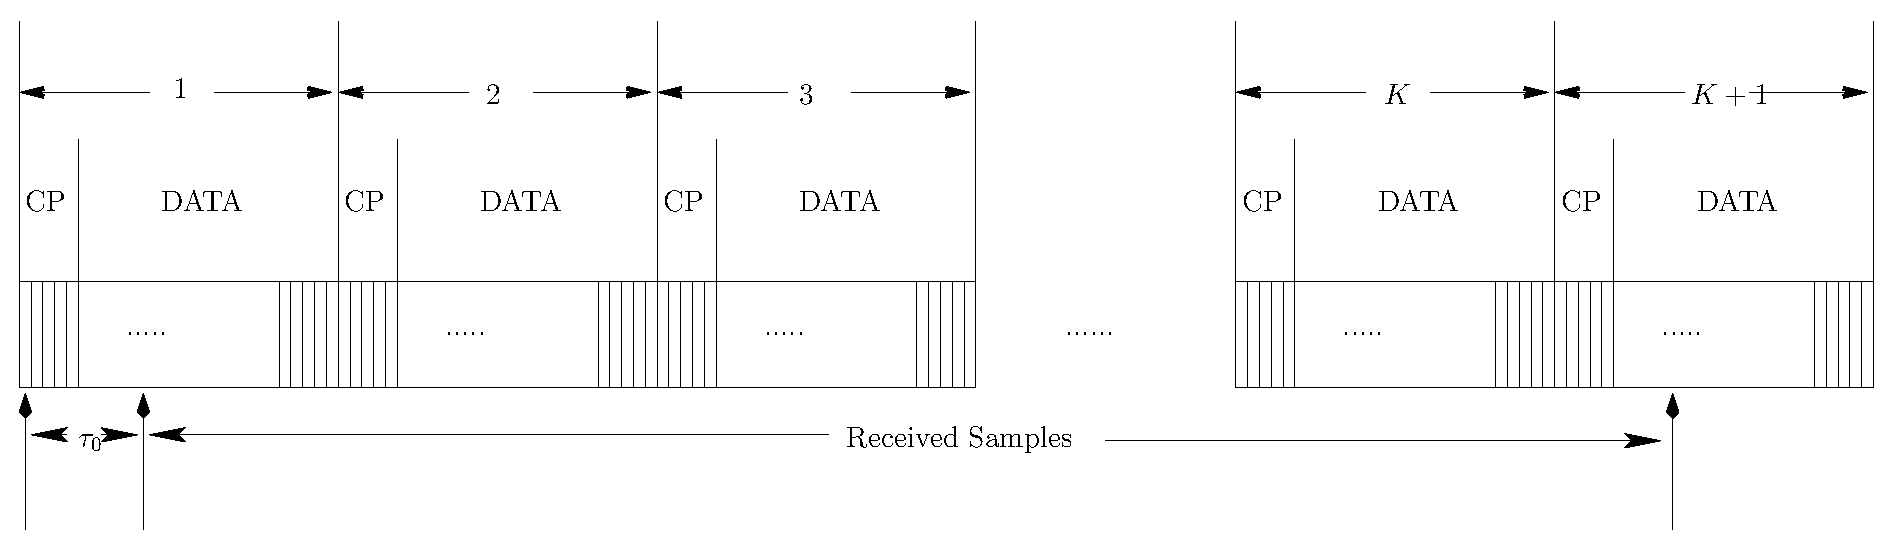
\includegraphics[width=\textwidth]{4/fig3.eps}
  \caption{Received signal for synchronization mismatch $\tau_0$.}
  \label{pic:1222a2}
\end{figure}
Assume $\tau = \tau_0$, let $\Theta_{\tau_0}$ denote the set of subscripts such that if $i \in \Theta_{\tau_0}$,  $s_i$ is a symbol of CP sequence. [To be added].
From Figure XX, we can see $i \in \Theta_{\tau_0}$ only if $i + \tau_0 \in [Ql_0, Ql_0+l_c -1]$ ($Q = 0, 1, \cdots, K-1$). 
Let $\Theta_{\tau_0}^k$ denotes set $\Theta_{\tau_0}$ subtract set $\{k\}$ ($k$ is also a subscript), i.e.
\begin{equation}
  \{i\in \Theta_{\tau_0}^k| i + \tau_0 \in [Ql_0, Ql_0+l_c -1] (Q = 0, 1, \cdots, K-1)\;\;\;\; \text{and}\;\;\;\; i\neq k\}
  \label{definitionof}
\end{equation}

Like in (c.f. ), we make following assumptions about the noise and signal: (1) all noise samples are i.i.d. mean zero circularly symmetric complex Gaussian (CSCG) with variance $\sigma_n^2$; (2) under hypothesis $H_1$ the transmitted signal symbols in the data sequence are i.i.d. zero mean CSCG with variance $\sigma_{s_A}^2$ (or $\sigma_{s_B}^2$ under hypothesis $H_2$); (3) if $s_i$ is a sample in CP sequence, then we have $s_i = s_{i+l_D}$. 

The CP structure could introduce strong cyclostationarity to the transmitted OFDM signals ($s_A$ or $s_B$) \cite{lunden2010robust}. 
Let $r_i=x_ix_j^\ast$ ($j=i+l_D$), \cite{lunden2007spectrum} shows $r_i$ exhibit cyclic property at frequency $\alpha = \frac{Q}{l_0}$ ($Q = \pm1, \pm2, \cdots$). In this case, we consider a single cyclic detector at frequency $\alpha = \frac{1}{l_0}$. 
Let $\mathbf{r}$ denote the vector of $r_i$, since the length of vector $\mathbf{x}$ is $M$, the length of $\mathbf{r}$ is $M - l_D$. For simple representation, let $N = M - l_D$.
Like in most related literature reviews (c.f. \cite{lunden2010robust} \cite{dandawate1994statistical}), the cyclic-covariance estimator for frequency $\alpha$ can be written as
\begin{equation}
  \hat{R}(l_D, \alpha) = \frac{1}{N}\sum_{i=0}^{N-1} r_ib_i\,.
  \label{cyclicR}
\end{equation}
where $b_i = \exp(-j2\pi\alpha i)$. 
The output of the measuring device is the real and imaginary part of the cyclic covariance estimator, i.e. 
\begin{equation}
  Y = \begin{bmatrix}
	R \\
	I
  \end{bmatrix}\,,
  \label{cyclic_cov}
\end{equation}
where 
\[
  R = \Re(\hat{R}(l_D, \alpha))
\]
and 
\[
  I = \Im(\hat{R}(l_D, \alpha))\,.
\]
By observing $y$, a realization  of $Y$, the testing device determines the status of the channel.
According to \cite{lunden2010robust}, $\hat{R}(l_D, \alpha)$ subjects to normal distribution for a large $K$, so $Y$ has the two-dimensional Gaussian distribution \cite{goodman1963statistical}.
Let $\bar{c}$ and $\tilde{c}$ denote the real and imaginary parts of a complex number $c$ respectively. Then, $b_i = \bar{b}_i + j\tilde{b}_i$  and $r_i = \bar{r}_i + j\tilde{r}_i$. 

The moment function of $\bar{r}_i, \tilde{r}_i$ are derived in \cite{axell2011optimal} and summarized in Table \ref{Table1} on page \pageref{Table1}.

% Please add the following required packages to your document preamble:
% \usepackage{multirow}
\begin{table}[h]
\centering
  \begin{tabular}{|c|c|c|c|c|c|}
	\hline
	\multirow{2}{*}{}           & \multirow{2}{*}{$H_0$} & \multicolumn{2}{c|}{$H_1$}                                                               & \multicolumn{2}{c|}{$H_2$}                                                               \\ \cline{3-6} 
	&                        & $i \in \Theta_{\tau_0}$                                                   & $i\notin \Theta_{\tau_0}$                          & $i\in \Theta_{\tau_0}$                                                   & $i\notin \Theta_{\tau_0}$                          \\ \hline
	$E[\bar{r}_i]$              & $0$                    & $2\sigma_{s_A}^2$                                       & $0$                            & $2\sigma_{s_B}^2$                                                         & $0$                            \\ \hline
	$E[\tilde{r}_i]$            & $0$                    & $0$                                                     & $0$                            & $0$                                                     & $0$                            \\ \hline
	$E[\bar{r}_i^2]$            & $2\sigma_n^4$          & $8\sigma_{s_A}^4+4\sigma_{s_A}^2\sigma_n^2+2\sigma_n^4$ & $2(\sigma_n^2+\sigma_{s_A}^2)^2$ & $8\sigma_{s_B}^4+4\sigma_{s_B}^2\sigma_n^2+2\sigma_n^4$ & $2(\sigma_n^2+\sigma_{s_B}^2)^2$ \\ \hline
	$E[\tilde{r}_i^2]$          & $2\sigma_n^4$          & $4\sigma_{s_A}^2\sigma_n^2+2\sigma_n^4$                 & $2(\sigma_n^2+\sigma_{s_A}^2)^2$ & $4\sigma_{s_B}^2\sigma_n^2+2\sigma_n^4$                 & $2(\sigma_n^2+\sigma_{s_B}^2)^2$ \\ \hline
	$E[\bar{r}_i\tilde{r}_i]$   & $0$                    & $0$                                                     & $0$                            & $0$                                                     & $0$                            \\ \hline
  \end{tabular}
  \caption{Moment function of $r_i$}
  \label{Table1}
\end{table}

Next we compute $E[\bar{r}_i\bar{r}_k]$, $E[\bar{r}_i\tilde{r}_k]$ and $E[\tilde{r}_i\tilde{r}_k]$ when $i \neq k$ under hypothesis $H_1$. For easy presentation, let $j = i+l_D$ and $l=k+l_D$.
 The expression of $r_i$ can be written as
\begin{equation}
  \begin{split}
    r_i = &(s_i+n_i)(s_j + n_j)^\ast\\
    = &(\bar{s}_i+j\tilde{s}_i + \bar{n}_i+j\tilde{n}_i)(\bar{s}_j-j\tilde{s}_j + \bar{n}_j-j\tilde{n}_j)\\
    = &\bar{s}_i\bar{s}_j + \bar{s}_i\bar{n}_j +\tilde{s}_i\tilde{s}_j+\tilde{s}_i\tilde{n}_j + \bar{n}_i\bar{s}_j+\bar{n}_i\bar{n}_j+\tilde{n}_i\tilde{s}_j+\tilde{n}_i\tilde{n}_j\\
    + &j\left( \tilde{s}_i\bar{s}_j + \tilde{s}_i\bar{n}_j + \tilde{n}_i\bar{s}_j + \tilde{n}_i\bar{n}_j - \bar{s}_i\tilde{s}_j - \bar{s}_i\tilde{n}_j - \bar{n}_i\tilde{s}_j - \bar{n}_i\tilde{n}_j \right)
  \end{split}
\end{equation}
thus we have 
\begin{equation}
  \begin{cases}
    \bar{r}_i = \bar{s}_i\bar{s}_j + \bar{s}_i\bar{n}_j +\tilde{s}_i\tilde{s}_j+\tilde{s}_i\tilde{n}_j + \bar{n}_i\bar{s}_j+\bar{n}_i\bar{n}_j+\tilde{n}_i\tilde{s}_j+\tilde{n}_i\tilde{n}_j\\
    \tilde{r}_i = \tilde{s}_i\bar{s}_j + \tilde{s}_i\bar{n}_j + \tilde{n}_i\bar{s}_j + \tilde{n}_i\bar{n}_j - \bar{s}_i\tilde{s}_j - \bar{s}_i\tilde{n}_j - \bar{n}_i\tilde{s}_j - \bar{n}_i\tilde{n}_j\,.
  \end{cases}
  \label{RrIr}
\end{equation}

\begin{equation}
  \begin{split}
    E[\bar{r}_i\bar{r}_k] = &E[(\bar{s}_i\bar{s}_j + \bar{s}_i\bar{n}_j +\tilde{s}_i\tilde{s}_j+\tilde{s}_i\tilde{n}_j + \bar{n}_i\bar{s}_j+\bar{n}_i\bar{n}_j+\tilde{n}_i\tilde{s}_j+\tilde{n}_i\tilde{n}_j)\\
    &(\bar{s}_k\bar{s}_l + \bar{s}_k\bar{n}_l +\tilde{s}_k\tilde{s}_l+\tilde{s}_k\tilde{n}_l + \bar{n}_k\bar{s}_l+\bar{n}_k\bar{n}_l+\tilde{n}_k\tilde{s}_l+\tilde{n}_k\tilde{n}_l)]\\
    = &E[\bar{s}_j\bar{s}_k\bar{s}_i\bar{s}_l]+E[\bar{s}_j\bar{s}_k\bar{s}_i\bar{n}_l]+E[\bar{s}_j\tilde{s}_k\bar{s}_i\tilde{s}_l]+E[\bar{s}_j\tilde{s}_k\bar{s}_i\tilde{n}_l]+E[\bar{s}_j\bar{n}_k\bar{s}_i\bar{s}_l]\\
&+E[\bar{s}_j\bar{n}_k\bar{s}_i\bar{n}_l]+E[\bar{s}_j\tilde{n}_k\bar{s}_i\tilde{s}_l]+E[\bar{s}_j\tilde{n}_k\bar{s}_i\tilde{n}_l]+E[\bar{n}_j\bar{s}_i\bar{s}_l\bar{s}_k]+E[\bar{n}_j\bar{s}_i\bar{n}_l\bar{s}_k]\\
&+E[\tilde{s}_k\bar{n}_j\bar{s}_i\tilde{s}_l]+E[\tilde{s}_k\bar{n}_j\bar{s}_i\tilde{n}_l]+E[\bar{n}_j\bar{n}_k\bar{s}_i\bar{s}_l]+E[\bar{n}_j\bar{n}_k\bar{s}_i\bar{n}_l]+E[\bar{n}_j\tilde{n}_k\bar{s}_i\tilde{s}_l]\\
&+E[\bar{n}_j\tilde{n}_k\bar{s}_i\tilde{n}_l]+E[\tilde{s}_j\tilde{s}_i\bar{s}_l\bar{s}_k]+E[\tilde{s}_j\tilde{s}_i\bar{n}_l\bar{s}_k]+E[\tilde{s}_k\tilde{s}_j\tilde{s}_i\tilde{s}_l]+E[\tilde{s}_k\tilde{s}_j\tilde{s}_i\tilde{n}_l]\\
&+E[\tilde{s}_j\tilde{s}_i\bar{n}_k\bar{s}_l]+E[\tilde{s}_j\tilde{s}_i\bar{n}_k\bar{n}_l]+E[\tilde{s}_j\tilde{s}_i\tilde{n}_k\tilde{s}_l]+E[\tilde{s}_j\tilde{s}_i\tilde{n}_k\tilde{n}_l]+E[\bar{s}_k\tilde{s}_i\tilde{n}_j\bar{s}_l]\\
&+E[\bar{s}_k\tilde{s}_i\tilde{n}_j\bar{n}_l]+E[\tilde{s}_k\tilde{s}_i\tilde{n}_j\tilde{s}_l]+E[\tilde{s}_k\tilde{s}_i\tilde{n}_l\tilde{n}_j]+E[\tilde{s}_i\bar{n}_k\tilde{n}_j\bar{s}_l]+E[\tilde{s}_i\bar{n}_k\tilde{n}_j\bar{n}_l]\\
&+E[\tilde{s}_i\tilde{n}_k\tilde{n}_j\tilde{s}_l]+E[\tilde{s}_i\tilde{n}_k\tilde{n}_l\tilde{n}_j]+E[\bar{n}_i\bar{s}_j\bar{s}_l\bar{s}_k]+E[\bar{n}_i\bar{s}_j\bar{n}_l\bar{s}_k]+E[\bar{n}_i\bar{s}_j\tilde{s}_k\tilde{s}_l]\\
&+E[\bar{n}_i\bar{s}_j\tilde{n}_l\tilde{s}_k]+E[\bar{n}_i\bar{s}_j\bar{n}_k\bar{s}_l]+E[\bar{n}_i\bar{s}_j\bar{n}_k\bar{n}_l]+E[\bar{n}_i\bar{s}_j\tilde{n}_k\tilde{s}_l]+E[\bar{n}_i\bar{s}_j\tilde{n}_k\tilde{n}_l]\\
&+E[\bar{n}_i\bar{s}_k\bar{n}_j\bar{s}_l]+E[\bar{n}_i\bar{s}_k\bar{n}_j\bar{n}_l]+E[\bar{n}_i\tilde{s}_k\bar{n}_j\tilde{s}_l]+E[\bar{n}_i\tilde{s}_k\bar{n}_j\tilde{n}_l]+E[\bar{n}_i\bar{n}_k\bar{n}_j\bar{s}_l]\\
&+E[\bar{n}_i\bar{n}_k\bar{n}_j\bar{n}_l]+E[\bar{n}_i\tilde{n}_k\bar{n}_j\tilde{s}_l]+E[\bar{n}_i\tilde{n}_k\bar{n}_j\tilde{n}_l]+E[\tilde{n}_i\bar{s}_k\bar{s}_l\tilde{s}_j]+E[\tilde{n}_i\bar{n}_l\bar{s}_k\tilde{s}_j]\\
&+E[\tilde{s}_k\tilde{n}_i\tilde{s}_l\tilde{s}_j]+E[\tilde{s}_k\tilde{n}_i\tilde{n}_l\tilde{s}_j]+E[\tilde{n}_i\bar{n}_k\bar{s}_l\tilde{s}_j]+E[\tilde{n}_i\bar{n}_k\bar{n}_l\tilde{s}_j]+E[\tilde{s}_l\tilde{n}_i\tilde{n}_k\tilde{s}_j]\\
&+E[\tilde{n}_i\tilde{n}_k\tilde{n}_l\tilde{s}_j]+E[\tilde{n}_i\tilde{n}_j\bar{s}_l\bar{s}_k]+E[\tilde{n}_i\tilde{n}_j\bar{n}_l\bar{s}_k]+E[\tilde{s}_k\tilde{n}_i\tilde{n}_j\tilde{s}_l]+E[\tilde{s}_k\tilde{n}_i\tilde{n}_j\tilde{n}_l]\\
&+E[\tilde{n}_i\tilde{n}_j\bar{n}_k\bar{s}_l]+E[\tilde{n}_i\tilde{n}_j\bar{n}_k\bar{n}_l]+E[\tilde{n}_i\tilde{n}_j\tilde{n}_k\tilde{s}_l]+E[\tilde{n}_i\tilde{n}_j\tilde{n}_k\tilde{n}_l]
  \end{split}
  \label{Erij}
\end{equation}
Since noise samples are governed by i.i.d Gaussian distribution with zero mean and they are independent with signals, items in \eqref{Erij} containing noise samples would have zero value, e.g. $E[\bar{s}_j\bar{s}_k\bar{s}_i\bar{n}_l] = E[\bar{s}_j\bar{s}_k\bar{s}_i]E[\bar{n}_l] = 0$. Eliminate zero value items in equation \eqref{Erij}:
\begin{equation}
  E[\bar{r}_i\bar{r}_k] = E[\bar{s}_i\bar{s}_j\bar{s}_k\bar{s}_l] + E[\bar{s}_i\bar{s}_j\tilde{s}_k\tilde{s}_l] + E[\tilde{s}_i\tilde{s}_j\bar{s}_k\bar{s}_l] + E[\tilde{s}_i\tilde{s}_j\tilde{s}_k\tilde{s}_l]
  \label{equ:Erirk}
\end{equation} 

Without losing generality, we assume $i < k$. Consider the situation when $k \notin \Theta_{\tau_0}$, in such case $s_k$ and $s_l$ are independent. It is easy to see $s_l$ is also independent with $s_i$ and $s_j$. Hence \eqref{equ:Erirk} can be written as
\begin{equation}
  \begin{split}
  E[\bar{r}_i\bar{r}_k] = &E[\bar{s}_i\bar{s}_j\bar{s}_k]E[\bar{s}_l] + E[\bar{s}_i\bar{s}_j\tilde{s}_k]E[\tilde{s}_l] + E[\tilde{s}_i\tilde{s}_j\bar{s}_k]E[\bar{s}_l] + E[\tilde{s}_i\tilde{s}_j\tilde{s}_k]E[\tilde{s}_l]\\
  = &0\,.
\end{split}
  \label{equ:Erirksitu1}
\end{equation} 
Similarly it can be proved when $i \notin \Theta_{\tau_0}$, we have $E[\bar{r}_i\bar{r}_k] =0$. Now consider the situation when $i, k \in \Theta_{\tau_0}$. In such case, we have 
\begin{equation}
  \begin{cases}
    s_i = s_j\\
    s_k = s_l
  \end{cases}
\end{equation}
and \eqref{equ:Erirk} can be written in form of
\begin{equation}
  \begin{split}
    E[\bar{r}_i\bar{r}_k] &= E[\bar{s}_i^2\bar{s}_k^2] + E[\bar{s}_i^2\tilde{s}_k^2]  +E[\tilde{s}_i^2\bar{s}_k^2] + E[\tilde{s}_i^2\tilde{s}_k^2] \\
    &= E[\bar{s}_i^2]E[\bar{s}_k^2] + E[\bar{s}_i^2]E[\tilde{s}_k^2]  +E[\tilde{s}_i^2]E[\bar{s}_k^2] + E[\tilde{s}_i^2]E[\tilde{s}_k^2] \\
    &= 4\sigma_{s_A}^4\,.
  \end{split}
  \label{Eririsitu2}
\end{equation}

From above discussion, the value of $E[\bar{r}_i\bar{r}_k]$  ($i \neq k$) can be summarized as
\begin{equation}
  E[\bar{r}_i\bar{r}_k] =  \begin{cases}
    4\sigma_{s_A}^4 \;\;\;\;&i, k \in \Theta_{\tau_0}\\
    0\;\;\;\;&\text{Otherwise}
  \end{cases}
  \label{Er_ir_j}
\end{equation}

Next consider $E[\bar{r}_i\tilde{r}_j]$, which can be written as
\begin{equation}
  \begin{split}
E[\bar{r}_i\tilde{r}_j] = &E[(\bar{s}_i\bar{s}_j + \bar{s}_i\bar{n}_j +\tilde{s}_i\tilde{s}_j+\tilde{n}_i\tilde{n}_j + \bar{n}_i\bar{s}_j+\bar{n}_i\bar{n}_j+\tilde{n}_i\tilde{s}_j+\tilde{n}_i\tilde{n}_j)\\
              &(\tilde{s}_k\bar{s}_l + \tilde{s}_k\bar{n}_l + \tilde{n}_k\bar{s}_l + \tilde{n}_k\bar{n}_l - \bar{s}_k\tilde{s}_l - \bar{s}_k\tilde{n}_l - \bar{n}_k\tilde{s}_l - \bar{n}_k\tilde{n}_l)]\,.
%              = &E[\bar{s}_j\tilde{s}_k\bar{s}_i\bar{s}_l]+E[\bar{s}_j\tilde{s}_k\bar{s}_i\bar{n}_l]+E[\bar{s}_j\tilde{n}_k\bar{s}_i\bar{s}_l]+E[\bar{s}_j\tilde{n}_k\bar{s}_i\bar{n}_l]-E[\bar{s}_j\bar{s}_k\bar{s}_i\tilde{s}_l]\\
%&-E[\bar{s}_j\bar{s}_k\bar{s}_i\tilde{n}_l]-E[\bar{s}_j\bar{n}_k\bar{s}_i\tilde{s}_l]-E[\bar{s}_j\bar{n}_k\bar{s}_i\tilde{n}_l]+E[\tilde{s}_k\bar{n}_j\bar{s}_i\bar{s}_l]+E[\tilde{s}_k\bar{n}_j\bar{s}_i\bar{n}_l]\\
%&+E[\bar{n}_j\tilde{n}_k\bar{s}_i\bar{s}_l]+E[\bar{n}_j\tilde{n}_k\bar{s}_i\bar{n}_l]-E[\tilde{s}_l\bar{n}_j\bar{s}_i\bar{s}_k]-E[\bar{n}_j\bar{s}_i\tilde{n}_l\bar{s}_k]-E[\bar{n}_j\bar{n}_k\bar{s}_i\tilde{s}_l]\\
%&-E[\bar{n}_j\bar{n}_k\bar{s}_i\tilde{n}_l]+E[\tilde{s}_k\tilde{s}_j\tilde{s}_i\bar{s}_l]+E[\tilde{s}_k\tilde{s}_j\tilde{s}_i\bar{n}_l]+E[\tilde{s}_j\tilde{s}_i\tilde{n}_k\bar{s}_l]+E[\tilde{s}_j\tilde{s}_i\tilde{n}_k\bar{n}_l]\\
%&-E[\tilde{s}_j\tilde{s}_i\tilde{s}_l\bar{s}_k]-E[\tilde{s}_j\tilde{s}_i\tilde{n}_l\bar{s}_k]-E[\tilde{s}_j\tilde{s}_i\bar{n}_k\tilde{s}_l]-E[\tilde{s}_j\tilde{s}_i\tilde{n}_l\bar{n}_k]+E[\tilde{s}_k\tilde{n}_i\tilde{n}_j\bar{s}_l]\\
%&+E[\tilde{s}_k\tilde{n}_i\tilde{n}_j\bar{n}_l]+E[\tilde{n}_i\tilde{n}_j\tilde{n}_k\bar{s}_l]+E[\tilde{n}_i\tilde{n}_j\tilde{n}_k\bar{n}_l]-E[\tilde{n}_i\tilde{n}_j\tilde{s}_l\bar{s}_k]-E[\tilde{n}_i\tilde{n}_j\tilde{n}_l\bar{s}_k]\\
%&-E[\tilde{n}_i\tilde{n}_j\bar{n}_k\tilde{s}_l]-E[\tilde{n}_i\tilde{n}_j\tilde{n}_l\bar{n}_k]+E[\bar{n}_i\bar{s}_j\bar{s}_l\tilde{s}_k]+E[\bar{n}_i\bar{s}_j\bar{n}_l\tilde{s}_k]+E[\bar{n}_i\bar{s}_j\tilde{n}_k\bar{s}_l]\\
%&+E[\bar{n}_i\bar{s}_j\tilde{n}_k\bar{n}_l]-E[\bar{n}_i\bar{s}_j\tilde{s}_l\bar{s}_k]-E[\bar{n}_i\bar{s}_j\tilde{n}_l\bar{s}_k]-E[\bar{n}_i\bar{s}_j\bar{n}_k\tilde{s}_l]-E[\bar{n}_i\bar{s}_j\bar{n}_k\tilde{n}_l]\\
%&+E[\bar{n}_i\tilde{s}_k\bar{n}_j\bar{s}_l]+E[\bar{n}_i\tilde{s}_k\bar{n}_j\bar{n}_l]+E[\bar{n}_i\tilde{n}_k\bar{n}_j\bar{s}_l]+E[\bar{n}_i\tilde{n}_k\bar{n}_j\bar{n}_l]-E[\bar{n}_i\bar{s}_k\bar{n}_j\tilde{s}_l]\\
%&-E[\bar{n}_i\bar{s}_k\bar{n}_j\tilde{n}_l]-E[\bar{n}_i\bar{n}_k\bar{n}_j\tilde{s}_l]-E[\bar{n}_i\bar{n}_k\bar{n}_j\tilde{n}_l]+E[\tilde{s}_k\tilde{n}_i\bar{s}_l\tilde{s}_j]+E[\tilde{s}_k\tilde{n}_i\bar{n}_l\tilde{s}_j]\\
%&+E[\tilde{n}_i\tilde{n}_k\bar{s}_l\tilde{s}_j]+E[\tilde{n}_i\tilde{n}_k\bar{n}_l\tilde{s}_j]-E[\tilde{n}_i\tilde{s}_l\bar{s}_k\tilde{s}_j]-E[\tilde{n}_i\tilde{n}_l\bar{s}_k\tilde{s}_j]-E[\tilde{n}_i\bar{n}_k\tilde{s}_l\tilde{s}_j]\\
%&-E[\tilde{n}_i\bar{n}_k\tilde{n}_l\tilde{s}_j]+E[\tilde{s}_k\tilde{n}_i\tilde{n}_j\bar{s}_l]+E[\tilde{s}_k\tilde{n}_i\tilde{n}_j\bar{n}_l]+E[\tilde{n}_i\tilde{n}_j\tilde{n}_k\bar{s}_l]+E[\tilde{n}_i\tilde{n}_j\tilde{n}_k\bar{n}_l]\\
%&-E[\tilde{n}_i\tilde{n}_j\tilde{s}_l\bar{s}_k]-E[\tilde{n}_i\tilde{n}_j\tilde{n}_l\bar{s}_k]-E[\tilde{n}_i\tilde{n}_j\bar{n}_k\tilde{s}_l]-E[\tilde{n}_i\tilde{n}_j\tilde{n}_l\bar{n}_k]
\end{split}
\label{Eriiiirk}
\end{equation}
expand \eqref{Eriiiirk} and eliminate zero value items (items including noise samples), we have 
 \begin{equation}
   E[\bar{r}_i\tilde{r}_k] = E[\bar{s}_j\tilde{s}_k\bar{s}_i\bar{s}_l] -  E[\bar{s}_j\bar{s}_k\bar{s}_i\tilde{s}_l] + E[\tilde{s}_j\tilde{s}_k\tilde{s}_i\bar{s}_l] - E[\tilde{s}_j\bar{s}_k\tilde{s}_i\tilde{s}_l]\,.
   \label{equ:1213a}
\end{equation}
Since the real and imaginary part of transmitted OFDM signals are independent and $E[\bar{s}_m] = E[\tilde{s}_m] = 0$ ($m = 0, 1, \cdots, N$), \eqref{equ:1213a} can be written as
\begin{equation}
  \begin{split}
  E[\bar{r}_i\tilde{r}_k] &= E[\tilde{s}_k]E[\bar{s}_i\bar{s}_j\bar{s}_l]  - E[\tilde{s}_l]E[\bar{s}_i\bar{s}_j\bar{s}_k] + E[\bar{s}_l]E[\tilde{s}_i\tilde{s}_j\tilde{s}_k] -  E[\bar{s}_k]E[\tilde{s}_i\tilde{s}_j\tilde{s}_l]\\
  &= 0
\end{split}
  \label{equ:1215m}
\end{equation}
thus we can see $E[\bar{r}_i\tilde{r}_k] = 0$  when $i \neq k $.  

Next consider $E[\tilde{r}_i\tilde{r}_k]$, which can be written as
\begin{equation}
  \begin{split}
    E[\tilde{r}_i\tilde{r}_k] = &E[(\tilde{s}_i\bar{s}_j + \tilde{s}_i\bar{n}_j + \tilde{n}_i\bar{s}_j + \tilde{n}_i\bar{n}_j - \bar{s}_i\tilde{s}_j - \bar{s}_i\tilde{n}_j - \bar{n}_i\tilde{s}_j - \bar{n}_i\tilde{n}_j)\\
    &(\tilde{s}_k\bar{s}_l + \tilde{s}_k\bar{n}_l + \tilde{n}_k\bar{s}_l + \tilde{n}_k\bar{n}_l - \bar{s}_k\tilde{s}_l - \bar{s}_k\tilde{n}_l - \bar{n}_k\tilde{s}_l - \bar{n}_k\tilde{n}_l)]
%    = &E[\bar{s}_j\tilde{s}_k\tilde{s}_i\bar{s}_l]+E[\bar{s}_j\tilde{s}_k\tilde{s}_i\bar{n}_l]+E[\bar{s}_j\tilde{s}_i\tilde{n}_k\bar{s}_l]+E[\bar{s}_j\tilde{s}_i\tilde{n}_k\bar{n}_l]-E[\bar{s}_j\bar{s}_k\tilde{s}_i\tilde{s}_l]\\
%&-E[\bar{s}_j\bar{s}_k\tilde{s}_i\tilde{n}_l]-E[\bar{s}_j\tilde{s}_i\bar{n}_k\tilde{s}_l]-E[\bar{s}_j\tilde{s}_i\tilde{n}_l\bar{n}_k]+E[\tilde{s}_k\tilde{s}_i\bar{n}_j\bar{s}_l]+E[\tilde{s}_k\tilde{s}_i\bar{n}_j\bar{n}_l]\\
%&+E[\tilde{n}_k\tilde{s}_i\bar{n}_j\bar{s}_l]+E[\tilde{n}_k\tilde{s}_i\bar{n}_j\bar{n}_l]-E[\bar{s}_k\tilde{s}_i\bar{n}_j\tilde{s}_l]-E[\bar{s}_k\tilde{s}_i\bar{n}_j\tilde{n}_l]-E[\tilde{s}_i\bar{n}_j\bar{n}_k\tilde{s}_l]\\
%&-E[\tilde{s}_i\bar{n}_j\tilde{n}_l\bar{n}_k]+E[\bar{s}_j\tilde{n}_i\bar{s}_l\tilde{s}_k]+E[\bar{s}_j\tilde{n}_i\bar{n}_l\tilde{s}_k]+E[\bar{s}_j\tilde{n}_i\tilde{n}_k\bar{s}_l]+E[\bar{s}_j\tilde{n}_i\tilde{n}_k\bar{n}_l]\\
%&-E[\bar{s}_j\tilde{n}_i\tilde{s}_l\bar{s}_k]-E[\bar{s}_j\tilde{n}_i\tilde{n}_l\bar{s}_k]-E[\bar{s}_j\tilde{n}_i\bar{n}_k\tilde{s}_l]-E[\bar{s}_j\tilde{n}_i\bar{n}_k\tilde{n}_l]+E[\tilde{s}_k\tilde{n}_i\bar{n}_j\bar{s}_l]\\
%&+E[\tilde{s}_k\tilde{n}_i\bar{n}_j\bar{n}_l]+E[\tilde{n}_i\tilde{n}_k\bar{n}_j\bar{s}_l]+E[\tilde{n}_i\tilde{n}_k\bar{n}_j\bar{n}_l]-E[\tilde{s}_l\tilde{n}_i\bar{n}_j\bar{s}_k]-E[\tilde{n}_i\bar{n}_j\tilde{n}_l\bar{s}_k]\\
%&-E[\tilde{n}_i\bar{n}_k\bar{n}_j\tilde{s}_l]-E[\tilde{n}_i\bar{n}_k\bar{n}_j\tilde{n}_l]-E[\tilde{s}_k\tilde{s}_j\bar{s}_i\bar{s}_l]-E[\tilde{s}_k\tilde{s}_j\bar{s}_i\bar{n}_l]-E[\tilde{s}_j\tilde{n}_k\bar{s}_i\bar{s}_l]\\
%&-E[\tilde{s}_j\tilde{n}_k\bar{s}_i\bar{n}_l]+E[\tilde{s}_l\tilde{s}_j\bar{s}_i\bar{s}_k]+E[\tilde{s}_j\bar{s}_i\tilde{n}_l\bar{s}_k]+E[\tilde{s}_j\bar{n}_k\bar{s}_i\tilde{s}_l]+E[\tilde{s}_j\bar{n}_k\bar{s}_i\tilde{n}_l]\\
%&-E[\tilde{s}_k\tilde{n}_j\bar{s}_i\bar{s}_l]-E[\tilde{s}_k\tilde{n}_j\bar{s}_i\bar{n}_l]-E[\tilde{n}_k\tilde{n}_j\bar{s}_i\bar{s}_l]-E[\tilde{n}_k\tilde{n}_j\bar{s}_i\bar{n}_l]+E[\bar{s}_k\tilde{n}_j\bar{s}_i\tilde{s}_l]\\
%&+E[\bar{s}_k\tilde{n}_j\bar{s}_i\tilde{n}_l]+E[\tilde{n}_j\bar{s}_i\bar{n}_k\tilde{s}_l]+E[\tilde{n}_j\bar{s}_i\tilde{n}_l\bar{n}_k]-E[\bar{n}_i\tilde{s}_j\bar{s}_l\tilde{s}_k]-E[\bar{n}_i\tilde{s}_j\bar{n}_l\tilde{s}_k]\\
%&-E[\bar{n}_i\tilde{s}_j\tilde{n}_k\bar{s}_l]-E[\bar{n}_i\tilde{s}_j\tilde{n}_k\bar{n}_l]+E[\bar{n}_i\tilde{s}_j\tilde{s}_l\bar{s}_k]+E[\bar{n}_i\tilde{s}_j\tilde{n}_l\bar{s}_k]+E[\bar{n}_i\tilde{s}_j\bar{n}_k\tilde{s}_l]\\
%&+E[\bar{n}_i\tilde{s}_j\bar{n}_k\tilde{n}_l]-E[\bar{n}_i\tilde{s}_k\tilde{n}_j\bar{s}_l]-E[\bar{n}_i\tilde{s}_k\tilde{n}_j\bar{n}_l]-E[\bar{n}_i\tilde{n}_j\tilde{n}_k\bar{s}_l]-E[\bar{n}_i\tilde{n}_j\tilde{n}_k\bar{n}_l]\\
%&+E[\bar{n}_i\bar{s}_k\tilde{n}_j\tilde{s}_l]+E[\bar{n}_i\bar{s}_k\tilde{n}_j\tilde{n}_l]+E[\bar{n}_i\tilde{n}_j\bar{n}_k\tilde{s}_l]+E[\bar{n}_i\tilde{n}_j\tilde{n}_l\bar{n}_k]
  \end{split}
  \label{EEEErrrrr}
\end{equation}
expand \eqref{EEEErrrrr} and eliminate zero value items (items including noise samples), we have 
\begin{equation}
  E[\tilde{r}_i\tilde{r}_k] = E[\bar{s}_j\tilde{s}_k\tilde{s}_i\bar{s}_l] -  E[\bar{s}_j\bar{s}_k\tilde{s}_i\tilde{s}_l] - E[\tilde{s}_j\tilde{s}_k\bar{s}_i\bar{s}_l] +E[\tilde{s}_j\bar{s}_k\bar{s}_i\tilde{s}_l]
  \label{1213night}
\end{equation}

Similar with $E[\bar{r}_i\bar{r}_k]$, when $i$ (or $k$) does not belong to set $\Theta_{\tau_0}$, we can see
$   E[\tilde{r}_i\tilde{r}_k] = 0$.

When $i, k \in \Theta_{\tau_0}$, equation \eqref{1213night} can be written as
\begin{equation}
  \begin{split}
  E[\tilde{r}_i\tilde{r}_k] = &E[\bar{s}_i\tilde{s}_k\tilde{s}_i\bar{s}_k] -  E[\bar{s}_i\bar{s}_k\tilde{s}_i\tilde{s}_k] - E[\tilde{s}_i\tilde{s}_k\bar{s}_i\bar{s}_k] +E[\tilde{s}_i\bar{s}_k\bar{s}_i\tilde{s}_k]\\
  = &E[\bar{s}_i]E[\tilde{s}_k]E[\tilde{s}_i]E[\bar{s}_k] -  E[\bar{s}_i]E[\bar{s}_k]E[\tilde{s}_i]E[\tilde{s}_k] - E[\tilde{s}_i]E[\tilde{s}_k]E[\bar{s}_i]E[\bar{s}_k] +E[\tilde{s}_i]E[\bar{s}_k]E[\bar{s}_i]E[\tilde{s}_k]\\
  = &0\,.
  \end{split}
\end{equation}
Hence we can conclude $E[\tilde{r}_i\tilde{r}_k] = 0$ when $i \neq k$. 

The statistics of $E[\bar{r}_i\bar{r}_k]$, $E[\bar{r}_i\tilde{r}_k]$ and $E[\tilde{r}_i\tilde{r}_k]$ under hypothesis $H_1$ are summarized in Table \ref{Table3} on page \pageref{Table3}. 
\begin{table}[h]
\centering
\begin{tabular}{|c|c|c|c|c|}
\hline
\multirow{2}{*}{Statistics} & \multicolumn{2}{c|}{$i = k$}                                                              & \multicolumn{2}{c|}{$i \neq k$}        \\ \cline{2-5} 
                            & $i\in \Theta_{\tau_0}$                                 & $i \notin \Theta_{\tau_0}$       & $i, k \in \Theta_{\tau_0}$ & Otherwise  \\ \hline
$E[\bar{r}_i\bar{r}_k]$     & $8\sigma_{s_A}^4+4\sigma_{s_A}^2\sigma_n^2+2\sigma_n^4$ & $2(\sigma_n^2+\sigma_{s_A}^2)^2$ & $4\sigma_{s_A}^4$          & $0$       \\ \hline
$E[\bar{r}_i\tilde{r}_k]$   & $0$                                                    & $0$                              & $0$                        & $0$       \\ \hline
$E[\tilde{r}_i\tilde{r}_k]$ & $4\sigma_{s_A}^2\sigma_n^2+2\sigma_n^4$                & $2(\sigma_n^2+\sigma_{s_A}^2)^2$ & $0$                        & $0$       \\ \hline
\end{tabular}
\caption{$E[\bar{r}_i\bar{r}_k]$, $E[\bar{r}_i\tilde{r}_k]$ and $E[\tilde{r}_i\tilde{r}_k]$ under hypothesis $H_1$}
\label{Table3}
\end{table}

In the following, we consider the distribution of $\begin{bmatrix}
  R \\
  I
\end{bmatrix}$ under hypothesis $H_1$ with synchronization mismatch $\tau = \tau_0$.
From the definition of $R$ and $I$, we have 
\begin{equation}
  \begin{split}
	R = &\Re{(\frac{1}{N}\sum_{i=0}^{N-1} b_ir_i)}\\
	= &\Re(\frac{1}{N}\sum_{i=0}^{N-1}(\bar{b}_i+j\tilde{b}_i)(\bar{r}_i+j\tilde{r}_i))\\
	= &\frac{1}{N}\sum_{i=0}^{N-1}\bar{b}_i\bar{r}_i - \frac{1}{N}\sum_{i=0}^{N-1}\tilde{b}_i\tilde{r}_i
  \end{split}
  \label{R}
\end{equation}
and
\begin{equation}
  \begin{split}
	I = &\Im(\frac{1}{N}\sum_{i=0}^{N-1} b_ir_i)\\
	= &\frac{1}{N}\sum_{i=0}^{N-1}\tilde{b}_i\bar{r}_i + \frac{1}{N}\sum_{i=0}^{N-1}\bar{b}_i\tilde{r}_i
  \end{split}
  \label{I}
\end{equation}

Let $a_i = \frac{1}{N}b_i$, then we have 
\begin{equation}
  \begin{cases}
	&R = \sum_{i=0}^{N-1}\bar{a}_i\bar{r}_i - \sum_{i=0}^{N-1}\tilde{a}_i\tilde{r}_i\\
	&I = \sum_{i=0}^{N-1}\tilde{a}_i\bar{r}_i +\sum_{i=0}^{N-1}\bar{a}_i\tilde{r}_i\,.
  \end{cases}
  \label{definitionofRI}
\end{equation}

Let $\mu_{R|\tau_0}$ $\mu_{I|\tau_0}$ denote the mean of $R$ and $I$ with synchronization mismatch $\tau=\tau_0$ respectively. By using the statistics of $r_i$ in Table \ref{Table1}, we compute  $\mu_{R|\tau_0}$ and  $\mu_{I|\tau_0}$:
\begin{equation}
  \begin{split}
	\mu_{R|\tau_0} =  E[R] = &\sum_{i=0}^{N-1}\bar{a}_iE[\bar{r}_i] - \sum_{i=0}^{N-1}\tilde{a}_iE[\tilde{r}_i]\\
	= &\sum_{i\in\Theta_{\tau_0}}\bar{a}_iE[\bar{r}_i]\\
	= &2\sigma_{s_A}^2\sum_{i\in\Theta_{\tau_0}}\bar{a}_i
  \end{split}
  \label{ER}
\end{equation}

\begin{equation}
  \begin{split}
	\mu_{I|\tau_0} =  E[I] = &\sum_{i=0}^{N-1}\tilde{a}_iE[\bar{r}_i] + \sum_{i=0}^{N-1}\bar{a}_iE[\tilde{r}_i]\\
	= &\sum_{i\in\Theta_{\tau_0}}\tilde{a}_iE[\bar{r}_i]\\
	= &2\sigma_{s_A}^2\sum_{i\in\Theta_0}\tilde{a}_i\,.
  \end{split}
  \label{EI}
\end{equation}

The  second order statistic of $R$ and $I$ can be computed as
\begin{equation}
  \begin{split}
	E[R^2] = &E[(\sum_{i=0}^{N-1}\bar{a}_i\bar{r}_i - \sum_{i=0}^{N-1}\tilde{a}_i\tilde{r}_i)(\sum_{i=0}^{N-1}\bar{a}_i\bar{r}_i - \sum_{i=0}^{N-1}\tilde{a}_i\tilde{r}_i)]\\
	= &E[\sum_{i=0}^{N-1}\sum_{k=0}^{N-1}\bar{a}_i\bar{a}_k\bar{r}_i\bar{r}_k - \sum_{i=0}^{N-1}\sum_{k=0}^{N-1}\bar{a}_i\tilde{a}_k\bar{r}_i\tilde{r}_k - \sum_{i=0}^{N-1}\sum_{k=0}^{N-1}\bar{a}_i\tilde{a}_k\bar{r}_i\tilde{r}_k + \sum_{i=0}^{N-1}\sum_{k=0}^{N-1}\tilde{a}_i\tilde{a}_k\tilde{r}_i\tilde{r}_k]\\
	= &\sum_{i=0}^{N-1}\sum_{k=0}^{N-1}\bar{a}_i\bar{a}_kE[\bar{r}_i\bar{r}_k] - \sum_{i=0}^{N-1}\sum_{k=0}^{N-1}\bar{a}_i\tilde{a}_kE[\bar{r}_i\tilde{r}_k] - \sum_{i=0}^{N-1}\sum_{k=0}^{N-1}\bar{a}_i\tilde{a}_kE[\bar{r}_i\tilde{r}_k] + \sum_{i=0}^{N-1}\sum_{k=0}^{N-1}\tilde{a}_i\tilde{a}_kE[\tilde{r}_i\tilde{r}_k]\,.
  \end{split}
  \label{ER^2}
\end{equation}
Substitute the statistics of $r_i$ in Table \ref{Table1}, Table \ref{Table3} and eliminate the zero elements, we have
\begin{equation}
  \begin{split}
	E[R^2]  
	= &\sum_{i=0}^{N-1}\bar{a}_i^2E[\bar{r}_i^2] + \sum_{i\in\Theta_{\tau_0}}\sum_{k\in\Theta_{\tau_0}^i}\bar{a}_i\bar{a}_kE[\bar{r}_i\bar{r}_k] + \sum_{i=0}^{N-1}\tilde{a}_i^2E[\bar{r}_i^2]\\
	= &\sum_{i\in\Theta_{\tau_0}}\bar{a}_i^2E[\bar{r}_i^2] + \sum_{i\in\Theta_{\tau_0}}\tilde{a}_i^2E[\tilde{r}_i^2] + \sum_{i\notin\Theta_{\tau_0}}(\bar{a}_i^2E[\bar{r}_i^2]+\tilde{a}_i^2E[\tilde{r}_i^2]) + \sum_{i\in\Theta_{\tau_0}}\sum_{k\in\Theta_{\tau_0}^i}\bar{a}_i\bar{a}_kE[\bar{r}_i\bar{r}_k]\\
	= &\sum_{i\in\Theta_{\tau_0}}\bar{a}_i^2(8\sigma_{s_A}^4+4\sigma_{s_A}^2\sigma_n^2+2\sigma_n^4) + \sum_{i\in\Theta_{\tau_0}}\tilde{a}_i^2(4\sigma_{s_A}^2\sigma_n^2+2\sigma_n^4) + \sum_{i\notin\Theta_{\tau_0}}(\tilde{a}_i^2+\bar{a}_i^2)2(\sigma_n^2+\sigma_{s_A}^2)^2\\
    &+4\sigma_{s_A}^4\sum_{i\in\Theta_{\tau_0}}\sum_{k\in\Theta_{\tau_0}^i}\bar{a}_i\bar{a}_k
  \end{split}
  \label{}
\end{equation}
From the definition of $a_i$ and $b_i$, we have
\begin{equation}
  \bar{a}_i^2 + \tilde{a}_i^2 =\frac{1}{N^2}
  \label{aisquare}
\end{equation}
hence \eqref{ER} can be written as
\begin{equation}
  \begin{split}
	E[R^2] = &\frac{1}{N^2}\sum_{i\in\Theta_{\tau_0}}  (4\sigma_{s_A}^2\sigma_n^2+2\sigma_n^4)+ 8\sum_{i\in\Theta_{\tau_0}}\bar{a}_i^2\sigma_{s_A}^4 + \frac{2}{N^2}\sum_{i\notin\Theta_{\tau_0}}(\sigma_n^2+\sigma_{s_A}^2)^2 + 4\sigma_{s_A}^4\sum_{i\in\Theta_{\tau_0}}\sum_{k\in\Theta_{\tau_0}^i}\bar{a}_i\bar{a}_k\\
	= &\frac{1}{N^2}\#\Theta_{\tau_0}(4\sigma_{s_A}^2\sigma_n^2+2\sigma_n^4) +  8\sum_{i\in\Theta_{\tau_0}}\bar{a}_i^2\sigma_{s_A}^4+ \frac{2}{N^2}(N - \#\Theta_{\tau_0})(\sigma_n^2+\sigma_{s_A}^2)^2\\
    &+4\sigma_{s_A}^4\sum_{i\in\Theta_{\tau_0}}\sum_{k\in\Theta_{\tau_0}^i}\bar{a}_i\bar{a}_k
  \end{split}
  \label{ER2}
\end{equation}
where $\#\Theta_{\tau_0}$ is the cardinality of set $\Theta_{\tau_0}$. 
Let $\sigma_{R|\tau_0}$ $\sigma_{I|\tau_0}$ denote the standard deviation of $R$ and $I$ when synchronization mismatch is $\tau_0$, 
\begin{equation}
  \begin{split}
	\sigma_{R|\tau_0} = &\sqrt{E[R^2] - E[R]^2}\\
	= &\left(\frac{1}{N^2}\#\Theta_{\tau_0}(4\sigma_{s_A}^2\sigma_n^2+2\sigma_n^4) + \frac{2}{N^2}(N - \#\Theta_{\tau_0})(\sigma_n^2+\sigma_{s_A}^2)^2 +  8\sigma_{s_A}^4\sum_{i\in\Theta_{\tau_0}}\bar{a}_i^2 \right.\\
  &\left.+ 4\sigma_{s_A}^4\sum_{i\in\Theta_{\tau_0}}\sum_{k\in\Theta_{\tau_0}^i}\bar{a}_i\bar{a}_k- \mu_{R|\tau_0}^2\right)^\frac{1}{2}\,.
  \end{split}
  \label{deviationR}
\end{equation}
Let $\beta_{\tau_0}^A = \frac{1}{N^2}\#\Theta_{\tau_0}(4\sigma_{s_A}^2\sigma_n^2+2\sigma_n^4) + \frac{2}{N^2}(N - \#\Theta_{\tau_0})(\sigma_n^2+\sigma_{s_A}^2)^2$ and above equation can be written as
\begin{equation}
  \sigma_{R|\tau_0} = \left(\beta_{\tau_0}^A+  8\sigma_{s_A}^4\sum_{i\in\Theta_{\tau_0}}\bar{a}_i^2 
    + 4\sigma_{s_A}^4\sum_{i\in\Theta_{\tau_0}}\sum_{k\in\Theta_{\tau_0}^i}\bar{a}_i\bar{a}_k- \mu_{R|\tau_0}^2\right)^\frac{1}{2}\,.
  \label{devR}
\end{equation}

Similarly, we compute $\sigma_{I|\tau_0}$ and $E[RI]$ as
\begin{equation}
  \begin{split}
	E[I^2] = &E[(\sum_{i=0}^{N-1}\tilde{a}_i\bar{r}_i + \sum_{i=0}^{N-1}\bar{a}_i\tilde{r}_i)(\sum_{i=0}^{N-1}\tilde{a}_i\bar{r}_i + \sum_{i=0}^{N-1}\bar{a}_i\tilde{r}_i)]\\
	= &\sum_{i=0}^{N-1}\sum_{k=0}^{N-1}\tilde{a}_i\tilde{a}_kE[\bar{r}_i\bar{r}_j] + \sum_{i=0}^{N-1}\sum_{k=0}^{N-1}\tilde{a}_i\bar{a}_jE[\bar{r}_i\tilde{r}_j] +\sum_{i=0}^{N-1}\sum_{k=0}^{N-1}\tilde{a}_i\bar{a}_jE[\bar{r}_i\tilde{r}_j] + \sum_{i=0}^{N-1}\sum_{k=0}^{N-1}\bar{a}_i\bar{a}_jE[\tilde{r}_i\tilde{r}_j] \\
	= &\sum_{i=0}^{N-1}(\bar{a}_i^2E[\tilde{r}^2] + \tilde{a}_i^2E[\bar{r}_i^2]) +4\sigma_{s_A}^4\sum_{i\in\Theta_{\tau_0}}\sum_{k\in\Theta_{\tau_0}^i}\tilde{a}_i\tilde{a}_k\\
	= &\frac{1}{N^2}\#\Theta_{\tau_0}(4\sigma_{s_A}^2\sigma_n^2+2\sigma_n^4) + \frac{2}{N^2}(N - \#\Theta_{\tau_0})(\sigma_n^2+\sigma_{s_A}^2)^2 +  8\sigma_{s_A}^4\sum_{i\in\Theta_{\tau_0}}\tilde{a}_i^2\\
    &+4\sigma_{s_A}^4\sum_{i\in\Theta_{\tau_0}}\sum_{k\in\Theta_{\tau_0}^i}\tilde{a}_i\tilde{a}_k
  \end{split}
  \label{EI^2}
\end{equation}
%\begin{equation}
%  E[I^2] = \sum_{i=0}^{N-1}(\bar{a}_i^2E[\tilde{r}^2] + \tilde{a}_i^2E[\bar{r}_i^2])
%  \label{EI2}
%\end{equation }
\begin{equation}
  \begin{split}
	\sigma_{I|\tau_0} = &\sqrt{E[I^2] - E[I]^2}\\
	= &\left(\frac{1}{N^2}\#\Theta_{\tau_0}(4\sigma_{s_A}^2\sigma_n^2+2\sigma_n^4) + \frac{2}{N^2}(N - \#\Theta_{\tau_0})(\sigma_n^2+\sigma_{s_A}^2)^2 +  8\sum_{i\in\Theta_{\tau_0}}\tilde{a}_i^2\sigma_{s_A}^4 \right.\\
	&\left.+ 4\sigma_{s_A}^4\sum_{i\in\Theta_{\tau_0}}\sum_{k\in\Theta_{\tau_0}^i}\tilde{a}_i\tilde{a}_k- \mu_{I|\tau_0}^2	\right)^\frac{1}{2}\\
    = &\left(\beta_{\tau_0}^A +  8\sigma_{s_A}^4\sum_{i\in\Theta_{\tau_0}}\tilde{a}_i^2+ 4\sigma_{s_A}^4\sum_{i\in\Theta_{\tau_0}}\sum_{k\in\Theta_{\tau_0}^i}\tilde{a}_i\tilde{a}_k- \mu_{I|\tau_0}^2	\right)^\frac{1}{2}\,.
  \end{split}
  \label{deviationI}
\end{equation}
\begin{equation}
  \begin{split}
	E[RI]= &E[\sum_{i=0}^{N-1} \sum_{k=0}^{N-1} \bar{a}_i\tilde{a}_k\bar{r}_i\bar{r}_k + 
	  \sum_{i=0}^{N-1} \sum_{k=0}^{N-1} \bar{a}_i\bar{a}_k\bar{r}_i\tilde{r}_k - 
	  \sum_{i=0}^{N-1} \sum_{k=0}^{N-1} \tilde{a}_i\tilde{a}_k\tilde{r}_i\bar{r}_k - 
	\sum_{i=0}^{N-1} \sum_{k=0}^{N-1} \tilde{a}_i\bar{a}_k\tilde{r}_i\tilde{r}_k]\\
	= &\sum_{i=0}^{N-1} \sum_{k=0}^{N-1} \bar{a}_i\tilde{a}_kE[\bar{r}_i\bar{r}_k] + 
	\sum_{i=0}^{N-1} \sum_{k=0}^{N-1} \bar{a}_i\bar{a}_kE[\bar{r}_i\tilde{r}_k] - 
	\sum_{i=0}^{N-1} \sum_{k=0}^{N-1} \tilde{a}_i\tilde{a}_kE[\tilde{r}_i\bar{r}_k] - 
	\sum_{i=0}^{N-1} \sum_{k=0}^{N-1} \tilde{a}_i\bar{a}_kE[\tilde{r}_i\tilde{r}_k]\\
	= &\sum_{i=0}^{N-1}\tilde{a}_i\bar{a}_iE[\bar{r}_i^2] - \sum_{i=0}^{N-1}\tilde{a}_i\bar{a}_iE[\tilde{r}_i^2] + 4\sigma_{s_A}^4\sum_{i\in\Theta_{\tau_0}}\sum_{k\in\Theta_{\tau_0}^i}\bar{a}_i\tilde{a}_k\\
	= &8\sigma_{s_A}^4\sum_{i\in \Theta_{\tau_0}}\tilde{a}_i\bar{a}_i+ 4\sigma_{s_A}^4\sum_{i\in\Theta_{\tau_0}}\sum_{k\in\Theta_{\tau_0}^i}\bar{a}_i\tilde{a}_k
	\label{ERI}
  \end{split}
\end{equation}
The last step comes from the fact that when $i \notin \Theta_{\tau_0}$, $E[\bar{r}_i^2] = E[\tilde{r}_i^2] = 2(\sigma_{s_A}^2 + \sigma_{n}^2)^2$.
Let $\rho_{\tau_0}$ represents the correlation between $R$ and $I$ when synchronization mismatch is $\tau_0$, we have
\begin{equation}
  \begin{split}
	\rho_{\tau_0} = &\frac{E[RI]-\mu_{R|\tau_0}\mu_{I|\tau_0}}{\sigma_{R|\tau_0}\sigma_{I|\tau_0}}\\
	= &\frac{8\sigma_{s_A}^4\sum_{i\in \Theta_{\tau_0}}\tilde{a}_i\bar{a}_i + 4\sigma_{s_A}^4\sum_{i\in\Theta_{\tau_0}}\sum_{k\in\Theta_{\tau_0}^i}\bar{a}_i\tilde{a}_k - \mu_{R|\tau_0}\mu_{I|\tau_0}}{\sigma_{R|\tau_0}\sigma_{I|\tau_0}}
  \end{split}
  \label{RIcorrelation}
\end{equation}
From \eqref{ER} and \eqref{EI} we have 
\begin{equation}
  \begin{split}
  \mu_{R|\tau_0}\mu_{I|\tau_0} = &4\sigma_{s_A}^4(\sum_{i\in\Theta_{\tau_0}}\bar{a}_i)(\sum_{i\in\Theta_{\tau_0}}\bar{a}_i)\\
  = &4\sigma_{s_A}^4\sum_{i\in\Theta_{\tau_0}}\sum_{k\in\Theta_{\tau_0}}\bar{a}_i\tilde{a}_k\\
  = &4\sigma_{s_A}^4\sum_{i\in\Theta_{\tau_0}}\sum_{k\in\Theta_{\tau_0}^i}\bar{a}_i\tilde{a}_k + 4\sigma_{s_A}^4\sum_{i\in\Theta_{\tau_0}}\bar{a}_i\tilde{a}_i
\end{split}
  \label{equ:1219n1}
\end{equation}
thus \eqref{ERI} can be written as
\begin{equation}
  \rho_{\tau_0}= \frac{4\sigma_{s_A}^4\sum_{i\in\Theta_{\tau_0}}\bar{a}_i\tilde{a}_i}{\sigma_{R|\tau_0}\sigma_{I|\tau_0}}\,.
  \label{ERI2}
\end{equation}
 
The distribution of 
$\begin{bmatrix}
  R \\
  I
\end{bmatrix}$ with synchronization mismatch $\tau = \tau_0$ can be written as
\begin{multline}
  f(R,I | \tau=\tau_0) = \frac{1}{2\pi\sigma_{I|\tau_0}\sigma_{R|\tau_0}\sqrt{1 - \rho_{\tau_0}^2}}\exp\left( -\frac{1}{2(1-\rho_{\tau_0}^2)}\left[ \frac{(R-\mu_{R|\tau_0})^2}{\sigma_{R|\tau_0}^2} + \right.\right.\\
  \left. \left.  \frac{(I-\mu_{I|\tau_0})^2}{\sigma_{I|\tau_0}^2} - \frac{2\rho(R-\mu_{R|\tau_0})(I-\mu_{I|\tau_0})}{\sigma_{R|\tau_0}\sigma_{I|\tau_0}}\right] \right)
  \label{disRI}
\end{multline}

In practise, the synchronization mismatch is governed by discrete niform distribution between $0$ and $l_0-1$. Hence in the situation of unknown $\tau$, the distribution of  
$\begin{bmatrix}
  R \\
  I
\end{bmatrix}$
under hypothesis $H_1$ can be written in form of 
\begin{equation}
  \begin{split}
	f_1(R, I) &= \sum_{\tau_0 = 0}^{l_0-1} \frac{1}{l_0}f(R, I|\tau=\tau_0)\\
	&= \sum_{\tau_0 = 0}^{l_0-1}\frac{1}{2l_0\pi\sigma_{I|\tau_0}\sigma_{R|\tau_0}\sqrt{1 - \rho_{\tau_0}^2}}\exp\left( -\frac{1}{2(1-\rho_{\tau_0}^2)}\left[ \frac{(R-\mu_{R|\tau_0})^2}{\sigma_{R|\tau_0}^2} + \right.\right.\\
	& \left. \left. \;\;\;\;\;\;\;\;\;\;\;\;\;\;\;\; \;\;\;\;\;\;\;\;\;\;\;\;\;\;\;\; \;\;\;\;\;\;\;\;\;\;\;\;\;\;\;\; \frac{(I-\mu_{I|\tau_0})^2}{\sigma_{I|\tau_0}^2} - \frac{2\rho(R-\mu_{R|\tau_0})(I-\mu_{I|\tau_0})}{\sigma_{R|\tau_0}\sigma_{I|\tau_0}}\right] \right)
  \end{split}
  \label{f_1underH1}
\end{equation}
and the statistic of $R$ and $I$  under hypothesis $H_1$ are summarized in Table \ref{Table2} on page \pageref{Table2}.
\begin{table}[h]
\centering
  \begin{tabular}{|c|c|}
	\hline
	Statistics          & Value                                                                                                                                                                                                                 \\ \hline
	$\mu_{R|\tau_0}$    & $\displaystyle{\sum_{i\in\Theta_{\tau_0}}\bar{a}_i2\sigma_{s_A}^2}$                                                                                                                                                                      \\ \hline
	$\mu_{I|\tau_0}$    & $\displaystyle{\sum_{i\in\Theta_0}\tilde{a}_i2\sigma_{s_A}^2}$                                                                                                                                                                           \\ \hline
    $\sigma_{R|\tau_0}$ & $\displaystyle{\left(\beta_{\tau_0}^A+8\sum_{i\in\Theta_{\tau_0}}\bar{a}_i^2\sigma_{s_A}^4 + 4\sigma_{s_A}^4\sum_{i\in\Theta_{\tau_0}}\sum_{k\in\Theta_{\tau_0}^i}\bar{a}_i\bar{a}_k- \mu_{R|\tau_0}^2 \right)^\frac{1}{2}}$  \\ \hline
    $\sigma_{I|\tau_0}$ & 
    $\begin{array} {l} \displaystyle{\left(\beta_{\tau_0}^A +8\sum_{i\in\Theta_{\tau_0}}\tilde{a}_i^2\sigma_{s_A}^4 +4\sigma_{s_A}^4\sum_{i\in\Theta_{\tau_0}}\sum_{k\in\Theta_{\tau_0}^i}\tilde{a}_i\tilde{a}_k- \mu_{R|\tau_0}^2\right)^\frac{1}{2}}\end{array}$ 
    \\ \hline
	$\rho_{\tau_0}$    & $ \displaystyle{\frac{4\sigma_{s_A}^4\sum_{i\in\Theta_{\tau_0}}\bar{a}_i\tilde{a}_i}{\sigma_{R|\tau_0}\sigma_{I|\tau_0}}}$                                                                            \\ \hline
  \end{tabular}
  \caption{Statistic for $R$ and $I$ under hypothesis $H_1$}
  \label{Table2}
\end{table}
Similarly the distribution of  
$\begin{bmatrix}
  R \\
  I
\end{bmatrix}$
under hypothesis $H_2$ can be written in form of 
\begin{equation}
  \begin{split}
	f_2(R, I) &= \sum_{\tau_0 = 0}^{l_0-1} \frac{1}{l_0}f(R, I|\tau=\tau_0)\\
	&= \sum_{\tau_0 = 0}^{l_0-1}\frac{1}{2l_0\pi\sigma_{I|\tau_0}\sigma_{R|\tau_0}\sqrt{1 - \rho_{\tau_0}^2}}\exp\left( -\frac{1}{2(1-\rho_{\tau_0}^2)}\left[ \frac{(R-\mu_{R|\tau_0})^2}{\sigma_{R|\tau_0}^2} + \right.\right.\\
	& \left. \left. \;\;\;\;\;\;\;\;\;\;\;\;\;\;\;\; \;\;\;\;\;\;\;\;\;\;\;\;\;\;\;\; \;\;\;\;\;\;\;\;\;\;\;\;\;\;\;\; \frac{(I-\mu_{I|\tau_0})^2}{\sigma_{I|\tau_0}^2} - \frac{2\rho(R-\mu_{R|\tau_0})(I-\mu_{I|\tau_0})}{\sigma_{R|\tau_0}\sigma_{I|\tau_0}}\right] \right)\,,
  \end{split}
  \label{f_2underH2}
\end{equation}
Let $\beta_{\tau_0}^B = \frac{1}{N^2}\#\Theta_{\tau_0}(4\sigma_{s_B}^2\sigma_n^2+2\sigma_n^4) + \frac{2}{N^2}(N - \#\Theta_{\tau_0})(\sigma_n^2+\sigma_{s_B}^2)^2$, 
the statistics of $R$ and $I$ under hypothesis $H_2$ are given in Table \ref{Table3} on page \pageref{Table3}. 
\begin{table}[h]
\centering
  \begin{tabular}{|c|c|}
	\hline
	Statistics          & Value                                                                                                                                                                                                                 \\ \hline
	$\mu_{R|\tau_0}$    & $\displaystyle{\sum_{i\in\Theta_{\tau_0}}\bar{a}_i2\sigma_{s_B}^2}$                                                                                                                                                                      \\ \hline
	$\mu_{I|\tau_0}$    & $\displaystyle{\sum_{i\in\Theta_0}\tilde{a}_i2\sigma_{s_B}^2}$                                                                                                                                                                           \\ \hline
    $\sigma_{R|\tau_0}$ & $\displaystyle{\left(\beta_{\tau_0}^B+8\sum_{i\in\Theta_{\tau_0}}\bar{a}_i^2\sigma_{s_B}^4 + 4\sigma_{s_B}^4\sum_{i\in\Theta_{\tau_0}}\sum_{k\in\Theta_{\tau_0}^i}\bar{a}_i\bar{a}_k- \mu_{R|\tau_0}^2 \right)^\frac{1}{2}}$  \\ \hline
    $\sigma_{I|\tau_0}$ & 
    $\begin{array} {l} \displaystyle{\left(\beta_{\tau_0}^B +8\sum_{i\in\Theta_{\tau_0}}\tilde{a}_i^2\sigma_{s_B}^4 +4\sigma_{s_B}^4\sum_{i\in\Theta_{\tau_0}}\sum_{k\in\Theta_{\tau_0}^i}\tilde{a}_i\tilde{a}_k- \mu_{R|\tau_0}^2\right)^\frac{1}{2}}\end{array}$ 
    \\ \hline
	$\rho_{\tau_0}$    & $ \displaystyle{\frac{4\sigma_{s_A}^4\sum_{i\in\Theta_{\tau_0}}\bar{a}_i\tilde{a}_i}{\sigma_{R|\tau_0}\sigma_{I|\tau_0}}}$                                                                            \\ \hline
  \end{tabular}
  \caption{Statistic for $R$ and $I$ under hypothesis $H_2$}
  \label{Table2}
\end{table}

Next we consider the distribution of 
$\begin{bmatrix}
  R \\
  I
\end{bmatrix}$
under hypothesis $H_0$. 
According to the expression of $R$ and $I$ given in \eqref{R} and \eqref{I}, $\mu_R$ and $\mu_I$ can be computed as
\begin{equation}
  \begin{split}
	\mu_R =E[R] = &\sum_{i=0}^{N-1}\bar{a}_iE[\bar{r}_i] - \sum_{i=0}^{N-1}\tilde{a}_iE[\tilde{r}_i] \\
	= &0
  \end{split}
  \label{ERnoise}
\end{equation}
and 
\begin{equation}
  \begin{split}
	\mu_{I|\tau_0} =  E[I] = &\sum_{i=0}^{N-1}\tilde{a}_iE[\bar{r}_i] + \sum_{i=0}^{N-1}\bar{a}_iE[\tilde{r}_i]\\
	= &0\,.
  \end{split}
  \label{EInoise}
\end{equation}
The second order statistics of $R$ and $I$ are
\begin{equation}
  \begin{split}
	E[R^2] = &E[(\sum_{i=0}^{N-1}\bar{a}_i\bar{r}_i - \sum_{i=0}^{N-1}\tilde{a}_i\tilde{r}_i)(\sum_{i=0}^{N-1}\bar{a}_i\bar{r}_i - \sum_{i=0}^{N-1}\tilde{a}_i\tilde{r}_i)]\\
	= &E[\sum_{i=0}^{N-1}\sum_{k=0}^{N-1}\bar{a}_i\bar{a}_k\bar{r}_i\bar{r}_k - \sum_{i=0}^{N-1}\sum_{k=0}^{N-1}\bar{a}_i\tilde{a}_k\bar{r}_i\tilde{r}_k - \sum_{i=0}^{N-1}\sum_{k=0}^{N-1}\bar{a}_i\tilde{a}_k\bar{r}_i\tilde{r}_k + \sum_{i=0}^{N-1}\sum_{k=0}^{N-1}\tilde{a}_i\tilde{a}_k\tilde{r}_i\tilde{r}_k]\\
	= &\sum_{i=0}^{N-1}\sum_{k=0}^{N-1}\bar{a}_i\bar{a}_kE[\bar{r}_i\bar{r}_k] - \sum_{i=0}^{N-1}\sum_{k=0}^{N-1}\bar{a}_i\tilde{a}_kE[\bar{r}_i\tilde{r}_k] - \sum_{i=0}^{N-1}\sum_{k=0}^{N-1}\bar{a}_i\tilde{a}_kE[\bar{r}_i\tilde{r}_k] + \sum_{i=0}^{N-1}\sum_{k=0}^{N-1}\tilde{a}_i\tilde{a}_kE[\tilde{r}_i\tilde{r}_k]\,.
    \end{split}
  \label{ER^2noise}
\end{equation}
Since all noise samples are independent and $r_i = n_i, r_k = n_k$,  we can see when $i/neq k$ $E[\bar{r}_i\bar{r}_k] = E[\bar{r}_i\tilde{r}_k] = E[\tilde{r}_i\tilde{r}_k] = 0$. The above equation can be simplified as 
\begin{equation}
\begin{split}
E[R^2] = &\sum_{i=0}^{N-1}(\bar{a}_i^2E[\bar{r}_i^2] + \tilde{a}_i^2E[\tilde{r}_i^2])\\
= &\frac{2\sigma_n^4}{N}\,.
\end{split}
\end{equation}
Similarly we have
\begin{equation}
  \begin{split}
	E[I^2] = &E[(\sum_{i=0}^{N-1}\tilde{a}_i\bar{r}_i + \sum_{i=0}^{N-1}\bar{a}_i\tilde{r}_i)(\sum_{i=0}^{N-1}\tilde{a}_i\bar{r}_i + \sum_{i=0}^{N-1}\bar{a}_i\tilde{r}_i)]\\
	= &\sum_{i=0}^{N-1}\sum_{k=0}^{N-1}\tilde{a}_i\tilde{a}_kE[\bar{r}_i\bar{r}_j] + \sum_{i=0}^{N-1}\sum_{k=0}^{N-1}\tilde{a}_i\bar{a}_jE[\bar{r}_i\tilde{r}_j] +\sum_{i=0}^{N-1}\sum_{k=0}^{N-1}\tilde{a}_i\bar{a}_jE[\bar{r}_i\tilde{r}_j] + \sum_{i=0}^{N-1}\sum_{k=0}^{N-1}\bar{a}_i\bar{a}_jE[\tilde{r}_i\tilde{r}_j] \\
	= &\sum_{i=0}^{N-1}(\bar{a}_i^2E[\tilde{r}^2] + \tilde{a}_i^2E[\bar{r}_i^2])\\
= &\frac{2\sigma_n^4}{N}\,.
  \end{split}
  \label{EI^2noise}
\end{equation}
and

\begin{equation}
  \begin{split}
	E[RI]= &E[\sum_{i=0}^{N-1} \sum_{k=0}^{N-1} \bar{a}_i\tilde{a}_k\bar{r}_i\bar{r}_k + 
	  \sum_{i=0}^{N-1} \sum_{k=0}^{N-1} \bar{a}_i\bar{a}_k\bar{r}_i\tilde{r}_k - 
	  \sum_{i=0}^{N-1} \sum_{k=0}^{N-1} \tilde{a}_i\tilde{a}_k\tilde{r}_i\bar{r}_k - 
	\sum_{i=0}^{N-1} \sum_{k=0}^{N-1} \tilde{a}_i\bar{a}_k\tilde{r}_i\tilde{r}_k]\\
	= &\sum_{i=0}^{N-1} \sum_{k=0}^{N-1} \bar{a}_i\tilde{a}_kE[\bar{r}_i\bar{r}_k] + 
	\sum_{i=0}^{N-1} \sum_{k=0}^{N-1} \bar{a}_i\bar{a}_kE[\bar{r}_i\tilde{r}_k] - 
	\sum_{i=0}^{N-1} \sum_{k=0}^{N-1} \tilde{a}_i\tilde{a}_kE[\tilde{r}_i\bar{r}_k] - 
	\sum_{i=0}^{N-1} \sum_{k=0}^{N-1} \tilde{a}_i\bar{a}_kE[\tilde{r}_i\tilde{r}_k]\\
	= 0\,.
	\label{ERInoise}
  \end{split}
\end{equation}
The standard deviation of $R$ and $I$ under hypothesis $H_0$ is
\begin{equation}
  \sigma_R = \sqrt{E[R^2] - E[R]^2} = \sqrt{\frac{2}{N}}\sigma_n^2
  \label{deviationRNOISE}
\end{equation}
and
\begin{equation}
  \sigma_I = \sqrt{E[I^2] - E[I]^2} = \sqrt{\frac{2}{N}}\sigma_n^2\,.
  \label{deviationR}
\end{equation}

Further more, since $E[RI] = E[R]E[I]$ = 0 and $R, I$ are combined gaussian distributed,  we know under hypothesis $H_0$ they are independent. Hence the distribution of $\begin{bmatrix}
  R \\
  I
\end{bmatrix}$ under hypothesis $H_0$ can be written as
\begin{equation}
  \begin{split}
	f_0(R, I)= &f_0(R)f_0(I)\\
	= &\frac{1}{\sqrt{\frac{2}{N}}\sigma_n^2\sqrt{2\pi}}\exp\left( -\frac{NR^2}{4\sigma_n^4} \right)\frac{1}{\sqrt{\frac{2}{N}}\sigma_n^2\sqrt{2\pi}}\exp\left( -\frac{NI^2}{4\sigma_n^4} \right)\\
	=&\frac{N}{4\pi \sigma_n^4}\exp\left( -\frac{NI^2+NR^2}{4\sigma_n^4} \right) 
  \end{split}
  \label{f0R0}
\end{equation}
\subsection{Numerical Results}

Assume $l_c = 4$ $l_d = 16$ $l_0 = 20$ and $K = 50$. We set the variance of noise is $\sigma_n^2 = 0.1$, the variance of signal $s_A$ and $s_B$ are $\sigma_{s_A} = 0.05$ and $\sigma_{s_B} = 0.3$ respectively. 
The value of $\mu_R$ $\mu_I$ $\sigma_R^2$ $\sigma_I^2$ and $\rho$ under hypotheses $H_1$ and $H_2$ are derived from Table \ref{Table3} and Table \ref{Table2} and illustrated in Table \ref{Table11} on page \pageref{Table11} and Table \ref{Table12} on page \pageref{Table12}. 
\begin{table}[h]
\begin{tabular}{|c|c|c|c|c|c|}
\hline
$\tau$ & $\mu_R$ & $\mu_I$ & $\sigma_R^2$ & $\sigma_I^2$ & $\rho$ \\
\hline
$ 0 $ & $ 1.7011e-02 $ &  $ -8.6678e-03 $ & $ 4.6199e-05 $ & $ 4.5265e-05 $ & $ -1.4058e-02 $ \\ 
$ 1 $ & $ 1.8761e-02 $ &  $ -3.0181e-03 $ & $ 4.6483e-05 $ & $ 4.4980e-05 $ & $ -5.4367e-03 $ \\ 
$ 2 $ & $ 1.8678e-02 $ &  $ 2.8956e-03 $ & $ 4.6482e-05 $ & $ 4.4982e-05 $ & $ 5.1965e-03 $ \\ 
$ 3 $ & $ 1.6773e-02 $ &  $ 8.4944e-03 $ & $ 4.6195e-05 $ & $ 4.5269e-05 $ & $ 1.3777e-02 $ \\ 
$ 4 $ & $ 1.3230e-02 $ &  $ 1.3230e-02 $ & $ 4.5732e-05 $ & $ 4.5732e-05 $ & $ 1.7029e-02 $ \\ 
$ 5 $ & $ 8.4944e-03 $ &  $ 1.6671e-02 $ & $ 4.5274e-05 $ & $ 4.6189e-05 $ & $ 1.3777e-02 $ \\ 
$ 6 $ & $ 2.9270e-03 $ &  $ 1.8480e-02 $ & $ 4.4991e-05 $ & $ 4.6472e-05 $ & $ 5.2629e-03 $ \\ 
$ 7 $ & $ -2.9270e-03 $ &  $ 1.8480e-02 $ & $ 4.4991e-05 $ & $ 4.6472e-05 $ & $ -5.2629e-03 $ \\ 
$ 8 $ & $ -8.4944e-03 $ &  $ 1.6671e-02 $ & $ 4.5274e-05 $ & $ 4.6189e-05 $ & $ -1.3777e-02 $ \\ 
$ 9 $ & $ -1.3230e-02 $ &  $ 1.3230e-02 $ & $ 4.5732e-05 $ & $ 4.5732e-05 $ & $ -1.7029e-02 $ \\ 
$ 10 $ & $ -1.6671e-02 $ &  $ 8.4944e-03 $ & $ 4.6189e-05 $ & $ 4.5274e-05 $ & $ -1.3777e-02 $ \\ 
$ 11 $ & $ -1.8480e-02 $ &  $ 2.9270e-03 $ & $ 4.6472e-05 $ & $ 4.4991e-05 $ & $ -5.2629e-03 $ \\ 
$ 12 $ & $ -1.8480e-02 $ &  $ -2.9270e-03 $ & $ 4.6472e-05 $ & $ 4.4991e-05 $ & $ 5.2629e-03 $ \\ 
$ 13 $ & $ -1.6671e-02 $ &  $ -8.4944e-03 $ & $ 4.6189e-05 $ & $ 4.5274e-05 $ & $ 1.3777e-02 $ \\ 
$ 14 $ & $ -1.3230e-02 $ &  $ -1.3230e-02 $ & $ 4.5732e-05 $ & $ 4.5732e-05 $ & $ 1.7029e-02 $ \\ 
$ 15 $ & $ -8.4944e-03 $ &  $ -1.6671e-02 $ & $ 4.5274e-05 $ & $ 4.6189e-05 $ & $ 1.3777e-02 $ \\ 
$ 16 $ & $ -2.9270e-03 $ &  $ -1.8480e-02 $ & $ 4.4991e-05 $ & $ 4.6472e-05 $ & $ 5.2629e-03 $ \\ 
$ 17 $ & $ 2.9867e-03 $ &  $ -1.8562e-02 $ & $ 4.4989e-05 $ & $ 4.6474e-05 $ & $ -5.3703e-03 $ \\ 
$ 18 $ & $ 8.6364e-03 $ &  $ -1.6813e-02 $ & $ 4.5274e-05 $ & $ 4.6189e-05 $ & $ -1.3992e-02 $ \\ 
$ 19 $ & $ 1.3469e-02 $ &  $ -1.3404e-02 $ & $ 4.5736e-05 $ & $ 4.5728e-05 $ & $ -1.7310e-02 $ \\ 
\hline
\end{tabular}
\caption{$\mu_R$ $\mu_I$ $\sigma_R^2$ $\sigma_I^2$ and $\rho$ under hypothesis $H_1$}
\label{Table11}
\end{table}

\begin{table}[h]
\begin{tabular}{|c|c|c|c|c|c|}
\hline
$\tau$ & $\mu_R$ & $\mu_I$ & $\sigma_R^2$ & $\sigma_I^2$ &$ \rho$ \\
\hline
$ 0 $ & $ 6.8046e-02 $ &  $ -3.4671e-02 $ & $ 1.9040e-04 $ & $ 1.7545e-04 $ & $ -5.6278e-02 $ \\ 
$ 1 $ & $ 7.5043e-02 $ &  $ -1.2072e-02 $ & $ 1.9495e-04 $ & $ 1.7090e-04 $ & $ -2.1791e-02 $ \\ 
$ 2 $ & $ 7.4714e-02 $ &  $ 1.1582e-02 $ & $ 1.9493e-04 $ & $ 1.7093e-04 $ & $ 2.0828e-02 $ \\ 
$ 3 $ & $ 6.7091e-02 $ &  $ 3.3978e-02 $ & $ 1.9033e-04 $ & $ 1.7552e-04 $ & $ 5.5151e-02 $ \\ 
$ 4 $ & $ 5.2922e-02 $ &  $ 5.2922e-02 $ & $ 1.8293e-04 $ & $ 1.8293e-04 $ & $ 6.8115e-02 $ \\ 
$ 5 $ & $ 3.3978e-02 $ &  $ 6.6685e-02 $ & $ 1.7560e-04 $ & $ 1.9025e-04 $ & $ 5.5150e-02 $ \\ 
$ 6 $ & $ 1.1708e-02 $ &  $ 7.3921e-02 $ & $ 1.7108e-04 $ & $ 1.9478e-04 $ & $ 2.1093e-02 $ \\ 
$ 7 $ & $ -1.1708e-02 $ &  $ 7.3921e-02 $ & $ 1.7108e-04 $ & $ 1.9478e-04 $ & $ -2.1093e-02 $ \\ 
$ 8 $ & $ -3.3978e-02 $ &  $ 6.6685e-02 $ & $ 1.7560e-04 $ & $ 1.9025e-04 $ & $ -5.5150e-02 $ \\ 
$ 9 $ & $ -5.2922e-02 $ &  $ 5.2922e-02 $ & $ 1.8293e-04 $ & $ 1.8293e-04 $ & $ -6.8115e-02 $ \\ 
$ 10 $ & $ -6.6685e-02 $ &  $ 3.3978e-02 $ & $ 1.9025e-04 $ & $ 1.7560e-04 $ & $ -5.5150e-02 $ \\ 
$ 11 $ & $ -7.3921e-02 $ &  $ 1.1708e-02 $ & $ 1.9478e-04 $ & $ 1.7108e-04 $ & $ -2.1093e-02 $ \\ 
$ 12 $ & $ -7.3921e-02 $ &  $ -1.1708e-02 $ & $ 1.9478e-04 $ & $ 1.7108e-04 $ & $ 2.1093e-02 $ \\ 
$ 13 $ & $ -6.6685e-02 $ &  $ -3.3978e-02 $ & $ 1.9025e-04 $ & $ 1.7560e-04 $ & $ 5.5150e-02 $ \\ 
$ 14 $ & $ -5.2922e-02 $ &  $ -5.2922e-02 $ & $ 1.8293e-04 $ & $ 1.8293e-04 $ & $ 6.8115e-02 $ \\ 
$ 15 $ & $ -3.3978e-02 $ &  $ -6.6685e-02 $ & $ 1.7560e-04 $ & $ 1.9025e-04 $ & $ 5.5150e-02 $ \\ 
$ 16 $ & $ -1.1708e-02 $ &  $ -7.3921e-02 $ & $ 1.7108e-04 $ & $ 1.9478e-04 $ & $ 2.1093e-02 $ \\ 
$ 17 $ & $ 1.1947e-02 $ &  $ -7.4250e-02 $ & $ 1.7105e-04 $ & $ 1.9480e-04 $ & $ -2.1524e-02 $ \\ 
$ 18 $ & $ 3.4546e-02 $ &  $ -6.7253e-02 $ & $ 1.7560e-04 $ & $ 1.9025e-04 $ & $ -5.6010e-02 $ \\ 
$ 19 $ & $ 5.3876e-02 $ &  $ -5.3615e-02 $ & $ 1.8299e-04 $ & $ 1.8286e-04 $ & $ -6.9240e-02 $ \\
\hline
\end{tabular}
\caption{$\mu_R$ $\mu_I$ $\sigma_R^2$ $\sigma_I^2$ and $\rho$ under hypothesis $H_2$}
\label{Table12}
\end{table}

By using \eqref{f_1underH1}, \eqref{f_2underH2} and \eqref{f0R0} we can compute the PDFs of  $\begin{bmatrix}
  R \\
  I
\end{bmatrix}$ under hypotheses $H_0$ $H_1$ and $H_2$, which are illustrated in Figure \ref{pic:1218n0} Figure \ref{pic:1218n1} Figure \ref{pic:1218n2} respectively. According to ENP test, the expression of $P_d$ $P_{f_1}$ and $P_{f_2}$ are
\begin{equation}
  \begin{cases}
	P_d = \int_{\infty}^\infty u(f_0(R,I) - k_1f_1(R,I) - k_2f_2(R,I))f_0(R,I)\mathrm{d}R\mathrm{d}I\\ 
	P_{f_1} = \int_{\infty}^\infty u(f_0(R,I) - k_1f_1(R,I) - k_2f_2(R,I))f_1(R,I)\mathrm{d}R\mathrm{d}I\\ 
	P_{f_2} = \int_{\infty}^\infty u(f_0(R,I) - k_1f_1(R,I) - k_2f_2(R,I))f_2(R,I)\mathrm{d}R\mathrm{d}I\,. 
  \end{cases}
  \label{asdffghj}
\end{equation}

We use look-up table method proposed in chapter 2 to compute the whole M-ROC.  Let $k_1$ $k_2$ increase from $0.1$ to $10000$ with step $0.1$ and store the corresponding $P_d, P_{f_1}$ and $P_{f_2}$ value in table $T_1$. For a given $c_1, c_2$, we iterate every item in table $T_1$ and put the item into table $T_2$ if the item satisfies: $P_{f_1} \leq c_1$ and $P_{f_2}\leq c_2$. After that, we iterate every item in table $T-2$ and get the largest $P_d$ in table $T_2$. The M-ROC is illustrated in figure \ref{1221n0}.  

\begin{figure}[!t]
  \centering 
  \includegraphics[width=12cm, height=16cm]{4/f0.eps}
  \caption{PDF under hypothesis $H_0$.}
  \label{pic:1218n0}
\end{figure}
\begin{figure}[!t]
  \centering 
  \includegraphics[width=12cm, height=16cm]{4/f1.eps}
  \caption{PDF under hypothesis $H_1$.}
  \label{pic:1218n1}
\end{figure}
\begin{figure}[!t]
  \centering 
  \includegraphics[width=12cm, height=16cm]{4/f2.eps}
  \caption{PDF under hypothesis $H_2$.}
  \label{pic:1218n2}
\end{figure}

\begin{figure}[!t]
  \centering 
  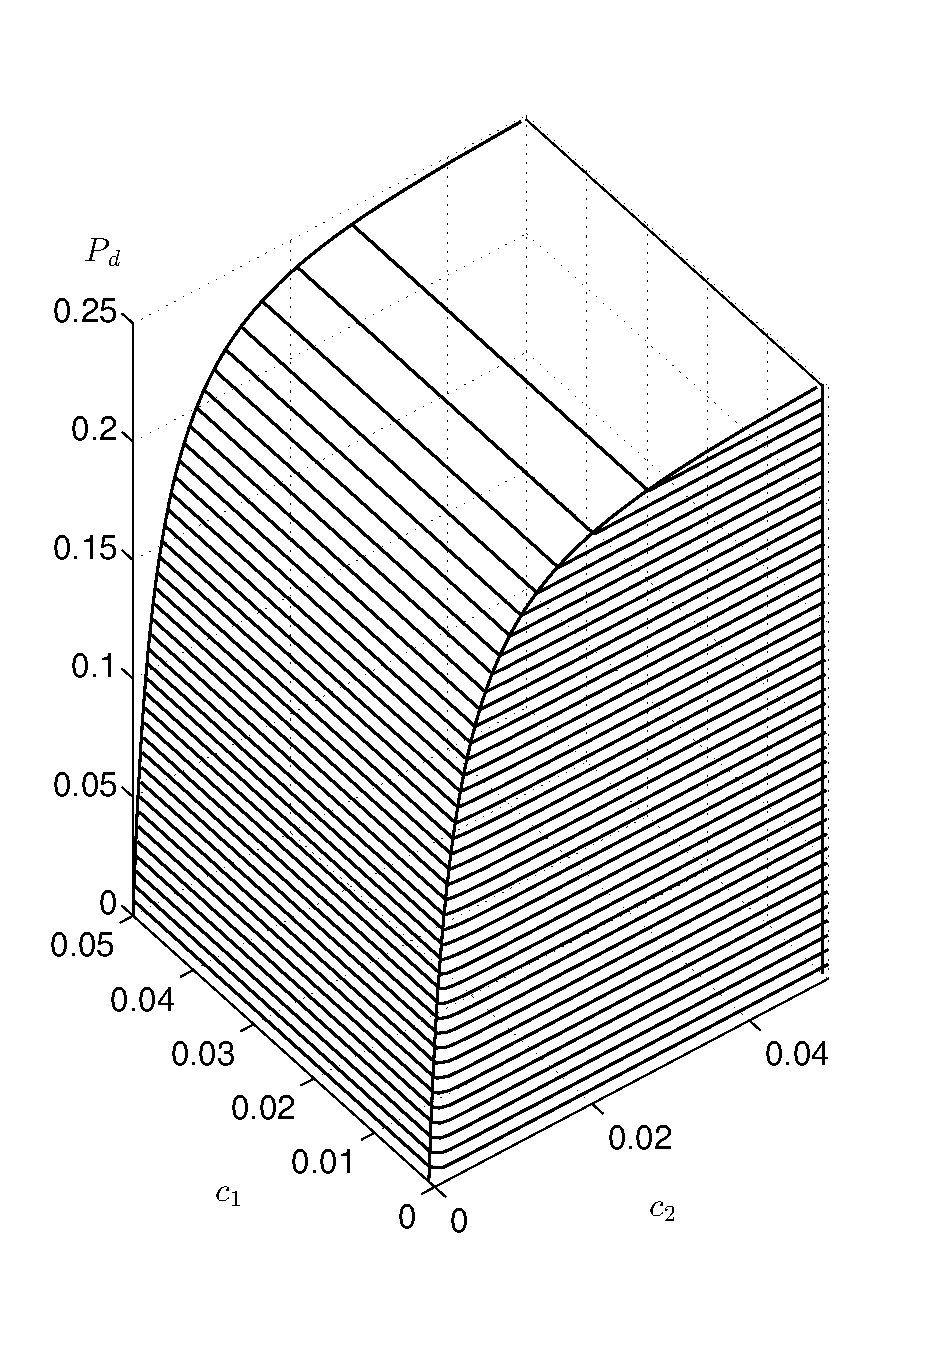
\includegraphics[width=12cm, height=16cm]{4/ROCsurface.eps}
  \caption{M-ROC surface for cyclostationary detector.}
  \label{pic:1221n0}
\end{figure}



%========== Appendices
%\appendix

%==========
%\typeout{}
%\resetdatestamp

\chapter{\LaTeX{}Macros}
\label{A:LaTeXmacros}

\section{Numerical Results Overview and Guide }
This section explains how to use the Matlab code that were used to generate the numerical results in this thesis. The capabilities are also discussed. The following table provides an overview of each source code file. All of these files can be found on the attached CD. 

\begin{table}[h]
\begin{tabular}{ll}
\hline
\hline
Source File Name                  & Description                                                                \\ \hline
gaussian\_example.m      & Generate ROC for normal Gaussian situation.              \\
Qian\_Zhang\_Algorithm.m & Implements Qian Zhang Algorithm to achieve MENP parameters.                \\
gaussian\_equal\_var.m   & Generate MROC for Gaussian distributions with equal variances. \\
gaussian\_situ.m         & Generate MROC for normal Gaussian situation.                   \\
JAchisquare.m            & Generate MROC for Chi-Square situation.                        \\
energy.m                 & Generate MROC for energy detection.                            \\
cyclodetection.m         & Generate MROC for cyclostationary detection.                 \\ 
\hline
\end{tabular}
\label{filelist}
\caption{Matlab source files}
\end{table}

To run a program, all of the files in Table \ref{filelist} in the Matlab current work folder. These programs have been successfully run using Matlab 2013b and Matlab 2014a on Linux platform with 12 GB RAM.  When execute JAchisquare.m, gaussiansitu.m or gaussianexample.m, the program loads configurations from init.txt file. When the computation finishes file output.mat stores the result and plotfigure.m execute automatically to generate associated figure. 

The adjustable parameters for ENP (MENP) test are listed in the following table. 


%========== Bibliography
\typeout{}
\begin{singlespace}
  \bibliography{ThesisEx}
  \bibliographystyle{ieeetr}
\end{singlespace}

\end{document}
